\documentclass[a4paper]{article}
\usepackage[spanish]{babel}
\usepackage[utf8]{inputenc}
\usepackage{charter}   % tipografia
\usepackage{graphicx}
%\usepackage{makeidx}
\usepackage{paralist} %itemize inline
\usepackage{amsmath}
%\usepackage[ruled,vlined,linesnumbered,resetcount,algochapter]{algorithm2e}
\usepackage{algorithm2e}
\usepackage{amssymb}

%\usepackage{float}
%\usepackage{amsmath, amsthm, amssymb}
%\usepackage{amsfonts}
%\usepackage{sectsty}
%\usepackage{charter}
%\usepackage{wrapfig}
%\usepackage{listings}
%\lstset{language=C}


\usepackage{color} % para snipets de codigo coloreados
\usepackage{fancybox}  % para el sbox de los snipets de codigo

\definecolor{litegrey}{gray}{0.94}

% \newenvironment{sidebar}{%
% 	\begin{Sbox}\begin{minipage}{.85\textwidth}}%
% 	{\end{minipage}\end{Sbox}%
% 		\begin{center}\setlength{\fboxsep}{6pt}%
% 		\shadowbox{\TheSbox}\end{center}}
% \newenvironment{warning}{%
% 	\begin{Sbox}\begin{minipage}{.85\textwidth}\sffamily\lite\small\RaggedRight}%
% 	{\end{minipage}\end{Sbox}%
% 		\begin{center}\setlength{\fboxsep}{6pt}%
% 		\colorbox{litegrey}{\TheSbox}\end{center}}

\newenvironment{codesnippet}{%
	\begin{Sbox}\begin{minipage}{\textwidth}\sffamily\small}%
	{\end{minipage}\end{Sbox}%
		\begin{center}%
		\vspace{-0.4cm}\colorbox{litegrey}{\TheSbox}\end{center}\vspace{0.3cm}}



\usepackage{fancyhdr}
\pagestyle{fancy}

%\renewcommand{\chaptermark}[1]{\markboth{#1}{}}
\renewcommand{\sectionmark}[1]{\markright{\thesection\ - #1}}

\fancyhf{}

\fancyhead[LO]{Sección \rightmark} % \thesection\ 
\fancyfoot[LO]{\small{Aldasoro Agustina, Bouz\'on Mar\'ia Bel\'en, Cairo Gustavo Juan}}
\fancyfoot[RO]{\thepage}
\renewcommand{\headrulewidth}{0.5pt}
\renewcommand{\footrulewidth}{0.5pt}
\setlength{\hoffset}{-0.8in}
\setlength{\textwidth}{16cm}
%\setlength{\hoffset}{-1.1cm}
%\setlength{\textwidth}{16cm}
\setlength{\headsep}{0.5cm}
\setlength{\textheight}{25cm}
\setlength{\voffset}{-0.7in}
\setlength{\headwidth}{\textwidth}
\setlength{\headheight}{13.1pt}

\renewcommand{\baselinestretch}{1.1}  % line spacing


% \setcounter{secnumdepth}{2}
\usepackage{underscore}
\usepackage{caratula}
\usepackage{url}


% ******************************************************** %
%              TEMPLATE DE INFORME ORGA2 v0.1              %
% ******************************************************** %
% ******************************************************** %
%                                                          %
% ALGUNOS PAQUETES REQUERIDOS (EN UBUNTU):                 %
% ========================================
%                                                          %
% texlive-latex-base                                       %
% texlive-latex-recommended                                %
% texlive-fonts-recommended                                %
% texlive-latex-extra?                                     %
% texlive-lang-spanish (en ubuntu 13.10)                   %
% ******************************************************** %



\begin{document}


\thispagestyle{empty}
\materia{M\'etodos Num\'ericos}
\submateria{Segundo Cuatrimestre de 2014}
\titulo{Trabajo Práctico II}
\subtitulo{Tirate un qu\'e, tirate un ranking...}
\integrante{Aldasoro Agustina}{86/13}{agusaldasoro@gmail.com}
\integrante{Bouz\'on Mar\'ia Bel\'en}{128/13}{belenbouzon@hotmail.com}
\integrante{Cairo Gustavo Juan}{89/13}{gjcairo@gmail.com}

\maketitle
\newpage

\thispagestyle{empty}
\vfill
\begin{abstract}
Habi\'endonos siendo dada la problem\'atica de c\'omo posicionar una p\'agina web alta en una b\'usqueda online, utilizando tres m\'etodos de ordenamiento de p\'aginas basados en links, este trabajo desarrolla distintas experimentaciones para la observaci\'on del comportamiento de los m\'etodos y de este modo saber cu\'al ser\'ia la tarea a llevar a cabo. \\
\\
\\
\indent \indent \textbf{Palabras claves} \\
\\
$\circ$ Matriz Esparsa \\
$\circ$ PageRank \\
$\circ$ HITS \\
$\circ$ In-deg \\

\end{abstract}

\thispagestyle{empty}
\vspace{3cm}
\tableofcontents
\newpage


%\normalsize
\newpage

\section{Introducci\'on Te\'orica}

A la hora de dise\~nar un Motor de B\'usqueda hay varios aspectos a tener en cuenta, tales como: contar con acceso a las p\'aginas disponibles en la red, tener una base de datos donde almacenarlas e indexarlas para su procesamiento posterior y ser capaces de ordenarlas de acuerdo a su importancia relativa dentro de dicha red. Nuestro trabajo se centrar\'a en este \'ultimo aspecto.

Existen varios m\'etodos que priorizan distintas caracter\'isticas de las relaciones entre las p\'aginas para dar cierto orden a una red a partir de determinada b\'usqueda. Un criterio v\'alido consiste en situar en una posici\'on de mayor jerarqu\'ia a aquellas p\'aginas que contengan mayor cantidad de coincidencias textuales con el concepto consultado. \'Este podr\'ia no resultar \'optimo en ciertos casos. Por ejemplo, si se buscara el string \textit{``Red Social''}, intuitivamente se esperar\'ia que entre los principales representantes de esta b\'usqueda se encontraran determinadas sitios web tales como Facebook o Twitter. Sin embargo, la cantidad de veces que estas p\'aginas contienen al string \textit{``Red Social''} puede no ser significativa y esto provocar\'ia que no aparecieran en los primeros lugares las p\'aginas genuinamente m\'as vinculadas al concepto buscado.

Todos los m\'etodos a desarrollar en este trabajo partir\'an del registro, la comparaci\'on y el an\'alisis de los Links Salientes/Entrantes  de la Red provista para ponderar el valor relativo de cada sitio en dicho sistema.
\\
\subsection{PageRank, HITS, In-deg}
El trabajo consistir\'a en el estudio de distintos aspectos de los siguientes m\'etodos: PageRank,
HITS e In-deg. Los mismos se detallan a continuaci\'on: \\
\\
\\
\indent \indent \emph{\textbf{PageRank} - Modelo del Navegante Aleatorio} \\
\indent Este m\'etodo consta de tres fases: exploraci\'on de la web y localizaci\'on todas las p\'aginas de acceso p\'ublico; indexado de los datos desde el primer paso, de manera que se pueda acceder eficientemente a palabras claves o frases relavantes; y valoraci\'on de la importancia de cada una de las p\'aginas en la base de datos. A nivel de nuestro desarrollo, s\'olo nos encargaremos de la \'ultima de las etapas mencionadas.\\
\indent Teniendo un grafo dirigido, se le otorga a cada componente $X_k$ del mismo un valor dado por la siguiente ecuaci\'on:
\[
 X_k = \sum_{j \epsilon L_k} \frac{X_j}{n_j}
\]
Donde\emph{ $L_k$} es el conjunto de links entrantes a la p\'agina k y \emph{$n_j$} es el n\'umero de links salientes desde la p\'agina j.\\
\indent Luego, se construye una matriz $A$ donde se encuentran -por filas- las respectivas ecuaciones para cada $X_i$, definidas como fue realizado anteriomente.\\
\indent La resoluci\'on de este m\'etodo se logra al hallar el autovector con autovalor asociado 1 para la matriz $A$. De acuerdo al trabajo de Bryan y Leise $[4]$, este c\'alculo se computa mediante el m\'etodo de la potencia. \\
\indent Dicha matriz cuenta con ciertas mejoras que proporcionan ventajas en casos espec\'ificos. Por un lado, si alguna p\'agina p no tuviera ning\'un link saliente se considera que el navegante aleatorio saltar\'a con equiprobabilidad a cualquiera de las otras p\'aginas. De esta forma, se le otorga al vector columna p de la matriz A el valor de $\frac{1}{n}$ para cada componente. Por otro lado, existe un fen\'omeno denominado \textit{``Teletransportaci\'on''} que considera la posibilidad de que dicho navegante se mueva de una p\'agina a otra pero no mediante los links existentes, sino tipeando la URL. Para modelar de manera \'optima este suceso, se reemplaza a la matriz A por la matriz M definida bajo la siguiente ecuaci\'on: \textit{M = (1-m)A + m.S} siendo m la probabilidad de que un navegante se \textit{teletransporte} y S una matriz cuyos valores $S_{ij}$ tienen todos el mismo valor: $\frac{1}{n}$ representando as\'i una matriz donde la probabilidad de ir a cualquier p\'agina del grafo es uniforme.\\
\indent El\emph{ M\'etodo de la Potencia} se realiza de manera iterativa, lo cual permite reducir el tiempo de c\'omputo para elevar a la k la matriz M. Si tenemos en cuenta el trabajo de Kamvar $[5]$, presenta una herramienta de c\'alculo que permite encontrar el principal autovector de M en una serie menor de pasos modificando la ecuaci\'on de la matriz M.\\
\\
\\
\indent \indent \emph{\textbf{Hyperlink-Induced Topic Search (HITS)}} \\
\indent El m\'etodo planteado por Kleinberg $[6]$ consiste en partir de una consulta sobre $\sigma$ y focalizarse en una colecci\'on de p\'aginas $S_\sigma$ tal que sea relativamente peque\~na,  rica en p\'aginas relevantes sobre el tema y contenga la mayor\'ia de las autoridades m\'as fuertes sobre el mismo. Considerando autoridad a una p\'agina que tiene la mayor cantidad de links entrantes provenientes de p\'aginas vinculadas al tema, esto se realiza del siguiente modo:\\
a) Acorde a un par\'ametro \emph{t}, se coleccionan las primeras t p\'aginas rankeadas bajo una b\'usqueda basada estrictamente por texto. A este conjunto se lo denomina $R_\sigma$. \\
b) Se incrementa el conjunto $R_\sigma$ a\~nadiendo las p\'aginas que tienen links entrantes y salientes al mismo, formando as\'i el conjunto $S_\sigma$. Para cada p\'agina de $R_\sigma$ se permite a\~nadir, a lo sumo \emph{d} p\'aginas que la apunten y \emph{d} p\'aginas a las cuales apunte. \\
c) Se eliminan de $S_\sigma$ los links intr\'insecos, es decir no se tienen en cuenta links que apuntan a una p\'agina del mismo dominio que la p\'agina saliente. \\
d) Se admiten hasta \emph{m} p\'aginas del mismo dominio apuntar a cualquier p\'agina p. Esta idea no fue utilizada por el autor. \\
\indent El conjunto obtenido hasta esta instancia lo llamamos $G_\sigma$. Nuestro trabajo asume un conjunto $G_\sigma$ bien formado.\\
\indent Se construye una matriz de adyacencia que denominaremos A, bajo la siguiente f\'ormula:
\[
   a_{ij} = 
   \begin{cases} 
      1              & \exists$\textit{ link desde i hasta j}$   \\
      0 & $\textit{caso contrario}$
   \end{cases}
\]
\indent A cada p\'agina i de la Web se le otorga un peso como Autoridad y un peso de Hub: \\
\indent \underline{Peso de autoridad:}
\[
	X_j = \sum_{i: i\rightarrow j}^{} Y_i
\]
\indent \underline{Peso de Hub:}
\[
Y_i = \sum_{j: i\rightarrow j} X_j
\]
\\
Este algoritmo devuelve dos arreglos: uno representa los pesos de Hub y otro los pesos de Autoridad, teniendo una coordenada para cada p\'agina perteneciente al conjunto $G_\sigma$.\\
\\
\\
\indent \indent \emph{\textbf{In-deg}} \\
\indent Consiste en definir el ranking de las p\'aginas utilizando s\'olo la cantidad de ejes entrantes a cada una de ellas, orden\'andolos en forma decreciente.\\

\newpage
\section{Desarrollo}
\subsection{Elecci\'on de las estructuras}

 Con el fin de elegir la estructura que representar\'ia nuestra matriz esparsa, estudiamos tres tipos proporcionados por la c\'atedra: \textit{Dictionary of Keys} (DOK), \textit{Compressed Sparse Row} (CSR) y \textit{Compressed Sparse Column} (CSC). \\
\indent La primera consiste en un diccionario con doble clave (fila y columna) y su significado son los elementos de la matriz distintos de cero. De esta manera se saca provecho de la cantidad de elementos nulos de la matriz, garantizando una optimizaci\'on en t\'erminos de espacio en memoria. Adem\'as esta implementaci\'on cuenta con la gran ventaja de que resulta simple construirla incrementalmente en un arreglo esparso y adem\'as puede ser traspuesta de manera sencilla (inviertiendo el orden de las claves). Sin embargo, el principal inconveniente reside en la necesidad de convertirla a otro formato para procesar los c\'alculos aritm\'eticos. A causa de esto fue descartada la opci\'on. \\
\indent El modo de almacenamiento \textit{Compressed Sparse Row} requiere la implementacion de tres arreglos (en nuestro caso vectores) que llamaremos val, ind_col y ptr_fila. El tamaño de los dos primeros est\'a dado por la cantidad de elementos no nulos de la matriz. Mientras que el primero (val) almacena estos valores de izquierda a derecha y luego desde arriba hacia abajo, el segundo vector (ind_col) indica el n\'umero de columna para cada elemento. En otras palabras, el elemento almacenado en la posici\'on i- \'esima del vector ind_col representa la columna correspondiente al valor almanacenado en val$_i$. Por \'ultimo el tercer vector (ptr_fila) tiene un tama\~no equivalente a la cantidad de filas incrementada en uno, conteniendo los \'indices del comienzo de cada fila.\\
\indent El modo de almacenamiento \textit{Compressed Sparse Column} cuenta tambi\'en con la implementaci\'on de tres arreglos llamados: val, ind_fila, ptr_col. El primero contiene todos los valores distintos de cero de la matriz, desde arriba hacia abajo y luego de izquierda a derecha. Ind_fila son los \'indices de fila correspondientes a dichos valores.  Por \'ultimo, ptr_col lista los \'indices donde comienza cada columna.\\
\indent Por \'ultimo, el tama\~no del vector ptr_fila se encuentra determinado por la cantidad de filas incrementada en uno, y lista los \'indices que indican los valores de val que comienzan cada fila.\\

 Ante a la disyuntiva acerca de cu\'al de estos \'ultimos formatos escoger (CSR o CSC) decidimos realizar una serie de c\'alculos peque\~nos que nos permitieron notar que si nos situ\'abamos en el formato de \textit{Compressed Spare}, trasponer una matriz almacenada de manera CSC no ser\'ia m\'as que interpretar sus mismos arreglos como CSC. Se incluye un ejemplo en \emph{Ap\'endice C}. Fue decisi\'on del grupo considerar el formato por defecto de la matriz el CSR (filas) y al trasponerlas s\'olo modificarle un bool que indique si est\'a traspuesta y leerla y considerarla en adelante como CSC (columnas). Esta decisi\'on fue tomada luego de que la c\'atedra nos confirmara que estaba permitido elegir una opci\'on de las ofrecidas y adaptarla a nuestra provecho, siempre que se aclararan los cambios. Por este motivo, en el algoritmo de multiplicar una matriz por un vector se diferencia la manera en que la misma se encuentre almacenada y se obtiene el producto acorde a su formato. Se incluye el pseudoc\'odigo de este algoritmo en la Subsecci\'on \emph{Algoritmo multiplicaci\'on de una matriz por un vector}. \\

\newpage
\subsection{Algoritmo multiplicaci\'on de una matriz por un vector}
 Considerando la estructura elegida, nos vemos obligados a diferenciar dentro del algoritmo de multiplicaci\'on de una matriz por un vector de acuerdo al modo en que debe ser le\'ido (CSR/CSC).\\
 \\
\indent Para computar el c\'alculo de una matriz por un vector interpret\'andolo bajo la estructura \emph{Compressed Sparse Row} se utiliz\'o el siguiente algoritmo: \\
\IncMargin{1em}
\begin{algorithm}
\SetKwData{Left}{left}\SetKwData{This}{this}\SetKwData{Up}{up}
\SetKwFunction{Union}{Union}\SetKwFunction{FindCompress}{FindCompress}
\SetKwInOut{Input}{input}\SetKwInOut{Output}{output}

\Input{Matriz m, Vector v}
\Output{Vector res}
\BlankLine
\For{$i\leftarrow 0$ \KwTo $cantidad$ $de$ $filas$}{
inicio $\leftarrow$ m.ptr_fil[i]\\
fin $\leftarrow$ m.ptr_fil[i+1]\\
\For{$j\leftarrow inicio$ \KwTo $fin$}{
col $\leftarrow$ m.ind_col[j]\\
res[i] $\leftarrow$ res[i] + (m.val[j] * v[col])\\
}
}
\end{algorithm}\DecMargin{1em}
\\
\textit{Se recorre el vector ptr_fil de la matriz, el cual indica en qu\'e \'indice comienza cada fila. Para cada elemento de la fila actual, se asigna en el int col el n\'umero de columna correspondiente; y luego, se multiplica ese elemento con el correspondiente del vector v (v[columna actual]) y se suma en res[i], siendo i la fila actual.}
\\
 \\
 \\
  \indent Para computar el c\'alculo de una matriz por un vector ley\'endolo bajo la estructura \emph{Compressed Sparse Column} se utiliz\'o el siguiente algoritmo: \\
   \\
\IncMargin{1em}
\begin{algorithm}
\SetKwData{Left}{left}\SetKwData{This}{this}\SetKwData{Up}{up}
\SetKwFunction{Union}{Union}\SetKwFunction{FindCompress}{FindCompress}
\SetKwInOut{Input}{input}\SetKwInOut{Output}{output}

\Input{Matriz m, Vector v}
\Output{Vector res}
\BlankLine
\For{$i\leftarrow 0$ \KwTo $cantidad$ $de$ $filas$}{
inicio $\leftarrow$ m.ptr_fil[i]\\
fin $\leftarrow$ m.ptr_fil[i+1]\\
\For{$j\leftarrow inicio$ \KwTo $fin$}{
fil $\leftarrow$ m.ind_col[j]\\
res[col] $\leftarrow$ res[fil] + (m.val[j] * v[i])\\
}
}
\end{algorithm}\DecMargin{1em}
\\

\textit{Se recorre el vector ptr_fil de la matriz, el cual indica en qu\'e \'indice comienza cada columna. Para cada elemento de la columna actual, se asigna en el int fil el n\'umero de fila correspondiente; y luego, se multiplica ese elemento con el correspondiente del vector v (v[fila Actual]) y se suma en res[fil].}\\


\newpage
\subsection{Algoritmo de HITS}

\indent Nuestra tarea aquí es extraer del subconjunto $G_\sigma$ sus autoridades analizando puramente la estructura de sus links. Ordenar las páginas, dándoles un puntaje de acuerdo a la cantidad de links de entrantes, trabaja mejor bajo el contexto de nuestro subconjunto, de todos modos un ranking de este tipo carece de una unidad temática. Las páginas con mayor puntaje de autoridad no solo tienen una cantidad significante de nodos entrantes sino que también van a tener muchas páginas en común que las apunten. \\
\indent Hubs y Autoridades reprensentan una relacion de mutua dependencia, frente a esto es necesario un método para solucionar este ciclo como el siguiente:\\

\IncMargin{1em}
\begin{algorithm}
\SetKwData{Left}{left}\SetKwData{This}{this}\SetKwData{Up}{up}
\SetKwFunction{Union}{Union}\SetKwFunction{FindCompress}{FindCompress}
\SetKwInOut{Input}{input}\SetKwInOut{Output}{output}

\Input{Matriz m, double tol}
\Output{Vector x, Vector y}
\BlankLine

Inicializar vectores \emph{x} e \emph{y} con 1 en todas sus posiciones\\
Vector xp, yp\\
\While{(No se haya llegado a la cantidad m\'axima de iteraciones i)}{

m.$trasponer()$ \\
xp $\leftarrow$ a.$multMatVect(y)$ \\
xp.$normalizar()$ \\
m.$trasponer()$ \\
yp $\leftarrow$ a.$multMatVect(x)$ \\
yp.$normalizar()$ \\
\eIf{(xp $\simeq$ x $\wedge$ yp $\simeq$ y)}{ 
			i $\leftarrow$ $M$\textit{\'a}$xima$ $Iteraci$\textit{\'o}$n$
		}{
			i++
		}
x $\leftarrow$ $xp$ \\
y $\leftarrow$ $yp$ \\
}
print \emph{x} e \emph{y}
\end{algorithm}\DecMargin{1em}

$\circ$Este algoritmo devuelve los valores de Autoridad y Hub para todas las p\'aginas, en X e Y respectivamente.\\
\indent $\circ$Los vectores X e Y arrancan inicializados en 1 \textcolor{blue}{ porque PINTO (??? GUSSSSSSSSS).}\\
\indent $\circ$El $\simeq$ considera la tolerancia (tol) pasada por parametro. Es decir, es equivalente a evaluar \\ abs(x-xp)$\leq$tol. \\
\indent $\circ$La cantidad m\'axima de iteraciones la fijamos nosotros en 100.000 pero al existir la guarda del if cabe la posibilidad de salir del scope del while antes de las 100.000 iteraciones. \\
\\
\indent El modelo de c\'alculo es un algoritmo iterativo, el cual conserva y actualiza los pesos de Hub y de Autoridad para cada p\'agina. Se cuenta con dos vectores de un tama\~no igual a la cantidad de nodos en la red, donde los pesos de autoridad de la p\'agina i se pueden ver en la posici\'on i del vector X, mientras que los de Hub se encuentran en la posici\'on i del vector Y. Ambos vectores son normalizados -bajo la Norma 2- en cada iteraci\'on. De este modo, las p\'aginas con mayor valor en X son ``mejores'' autoridades y las que tengan mayor valor en Y son ``mejores'' Hubs. \\
\indent Lo que se hace en cada iteraci\'on es actualizar primero los valores de X en base a los de Y, y luego actualizar los de Y en base a los nuevos de X. Se tiene una matriz A -\textit{Matriz de adyacencia}- la cual posee un 1 en A(i,j) si existe un link i $\rightarrow$ j y un 0 en caso contrario. De este modo, trasponi\'endola se puede observar la relaci\'on inversa. Esto explica que a la hora de actualizar los valores de X e Y se puede realizar asignando X $\leftarrow$ A$^t$Y, Y $\leftarrow$ AX; acorde a lo visto en la \emph{Introducci\'on Te\'orica} sobre el \textit{Algoritmo de HITS} se adaptan las ecuaciones a la forma matricial.\\ 
\indent Bas\'andonos en el trabajo de Kleinberg $[6]$, podemos asegurar que este m\'etodo converge bajo ciertas hip\'otesis \textcolor{blue}{(ESTOY MANDANDO FRUTA?)} como que el grafo $G_\sigma$ sea un grafo bien formado y que la matriz A tiene como principal autovector un valor \'unico \textcolor{blue}{(CREO QUE NADA MAS. PREGUNTAR A GUS.)}. En el mismo trabajo se puede ver la demostraci\'on  de que los vectores X e Y convergen a X* e Y*, y adem\'as X* es el principal autovector de A$^t$A e Y* es el principal autovector de AA$^t$.\\
\\
\indent Si bien nosotros optamos por devolver todos los puntajes de Hub y de Autoridad, al momento de emplearlo en una b\'usqueda de p\'aginas web se sit\'uan primero las \emph{k} mayores Autoridades y luego los \emph{k} mayores Hubs.


\newpage
\subsection{Algoritmo de PageRank}


\indent En este esquema, cada p\'agina se define como la suma de los valores de las p\'aginas con links entrantes divididos por su cantidad de enlaces salientes (modelo visto en la Introducci\'on te\'orica). La matriz a abordar se arma por columnas, para cada columna X$_i$ se pone un 0 en los elementos que no los dirija ning\'un link y $1/k$ en los dem\'as, siendo $k$ la cantidad de links salientes de la p\'agina X$_i$. Algo debe hacerse para solventar el problema de las p\'aginas con dangling nodes (p\'aginas sin ning\'un link saliente).\\
\indent Al contar con la matriz A -matriz de conectividad-, nuestro problema a resolver se limita a encontrar un autovector de A con autovalor 1. En el trabajo de Bryan y Leise $[4]$ se demuestra que: Si la Web con la que trabajamos no presenta ning\'un danglin node, la matriz de conectividad A tiene al 1 como autovalor mediante las siguientes preposiciones: \emph{La matriz A para alguna Web sin dangling nodes es estoc\'astica por columnas} (una matriz cuadrada es estoc\'astica por columnas si todos sus valores son no-negativos y los elementos de cada columna suman 1) y \emph{Toda matriz estoc\'astica por columnas tiene al 1 como autovalor}. Para asegurar la unicidad del ranking a armar es concluyente exigir que autovalor 1 tenga multiplicidad 1. \\
\indent Pero nosotros vamos a reemplazar A por M, la cual est\'a definida por la f\'ormula M = (1-m)A +  mS, con m la probabilidad de moverme entre p\'aginas no por medio de links y S una matriz con todos sus componentes iguales a 1/n. Donde as\'i no debe efectuarse ninguna hip\'otesis fuerte sobre A ya que M queda estoc\'astica por columnas y positiva la multiplicidad de $\lambda_1$ es 1. \\
\indent A fines de emplear menos recursos de c\'omputo se opt\'o por llevar a cabo el algoritmo desarrollado por Kamvar $[5]$:

\IncMargin{1em}
\begin{algorithm}
\SetKwData{Left}{left}\SetKwData{This}{this}\SetKwData{Up}{up}
\SetKwFunction{Union}{Union}\SetKwFunction{FindCompress}{FindCompress}
\SetKwInOut{Input}{input}\SetKwInOut{Output}{output}

\Input{Matriz m, double c, double tol}
\Output{x}
\BlankLine

Se inicializa el vector x en todos unos \\
Vector xp\\
\While{(No se haya llegado a la cantidad m\'axima de iteraciones i)}{
xp $\leftarrow$ m.$MultMatVec(x)$ \\
\For{$i\leftarrow 0$ \KwTo $tama$\textit{\~n}$o$ $de$ $xp$}{
xp[i] $\leftarrow$ xp[i] * c \\
}
\For{$i\leftarrow 0$ \KwTo $tama$\textit{\~n}$o$ $de$ $xp$}{
			xp[i] $\leftarrow$ $xp[i] + \frac{norma(x) - norma(xp)}{n}$
}
\eIf{(xp $\simeq$ x)}{ 
			i $\leftarrow$ \textit{M\'axima Iteraci\'on}
		}{
			i++
		}
x $\leftarrow$ xp

}
normalizar el vector \emph{x} \\
print \emph{x}
\end{algorithm}\DecMargin{1em}

$\circ$Este algoritmo devuelve el vector X el cual tiene Norma1 = 1 y representa para cada $X_i$ el porcentaje de tiempo que el \textit{Navegante Aleatorio} permanece en cada p\'agina i. \\
\indent $\circ$En este algoritmo no hace falta normalizar en cada iteraci\'on ya que conserva la norma.\\
\indent $\circ$El $\simeq$ considera la tolerancia (tol) pasada por parametro. Es decir, es equivalente a evaluar \\ abs(x-xp)$\leq$tol. \\
\indent $\circ$La cantidad m\'axima de iteraciones la fijamos nosotros en 1.000.000 pero al existir la guarda del if cabe la posibilidad de salir del scope del while antes del 1.000.000 de iteraciones. \\
\indent $\circ$ el par\'ametro C de entrada corresponde a la probabilidad de \textit{teletransportarse}.\\
\\
Lo que se calcula en este algoritmo es $X_k = M X_{k+1}$ mediante el m\'etodo de la potencia pero no se ejecuta la multiplicaci\'on de matrices sino que se hacen todos c\'alculos con vectores.

\newpage
\section{Resultados y discusi\'on}
\subsection{Convergencia de PageRank}

\textcolor{red}{INCLUIR EXPERIMENTOS SOBRE LA PROPORCION DEL LAMBDA. Cuanto mas se acerca a 1 (xq lambda uno es uno) mas tarda en converger.}

Estudio de la convergencia de PageRank, analizando la evolución de la norma Manhattan.\\
\textbf{Hip\'otesis}: Suponiendo que el método de la potencia converge (dado que la probabilidad de que no ocurra es minima), consideramos que la norma Manhattan de la diferencia entre iteraciones sucesivas debe converger a cero. Creemos que cuanto mayor sea el valor de c, más va a tardar en converger.\\
\\
\indent Nuestra hip\'otesis se bas\'o en la ecuaci\'on $P_2= cP_1+(1-c)E$, la cual hace que los datos cobren sentido. Dado un c, el segundo t\'ermino queda constante; por lo tanto, podemos considerarlo despreciable para nuestros cálculos, restringiéndonos a analizar lo que pueda suceder s\'olo con el primero. $cP_1$ implica la multiplicación de una matriz por un valor c tal que $0 \leq c \leq 1$. No resulta relevante considerar los casos en que $c= 0$ \'o $c=1$, dado que esos valores no modelarían un aspecto de la realidad. Esto se debe a que si $c=0$, la probabilidad de teletransportarse es 1 por lo tanto se moldear\'ia una realidad donde nunca se viaja a trav\'es de Links. Y por otro lado, si $c=1$ no se estar\'ia considerando la \emph{teletransportaci\'on}. \\
\indent Dado que c se encuentra entre $0$ y $1$, el resultado va a ser un vector de valores muy pequeños, que va a achicarse progresivamente. Es m\'as significativo lo que achica el c a $P_2$ que lo que aporta el segundo t\'ermino.   \\
\\
Los siguientes gr\'aficos est\'an citados en orden creciente de tama\~no de las redes:\\

\begin{figure}[h!]
  \begin{center}
	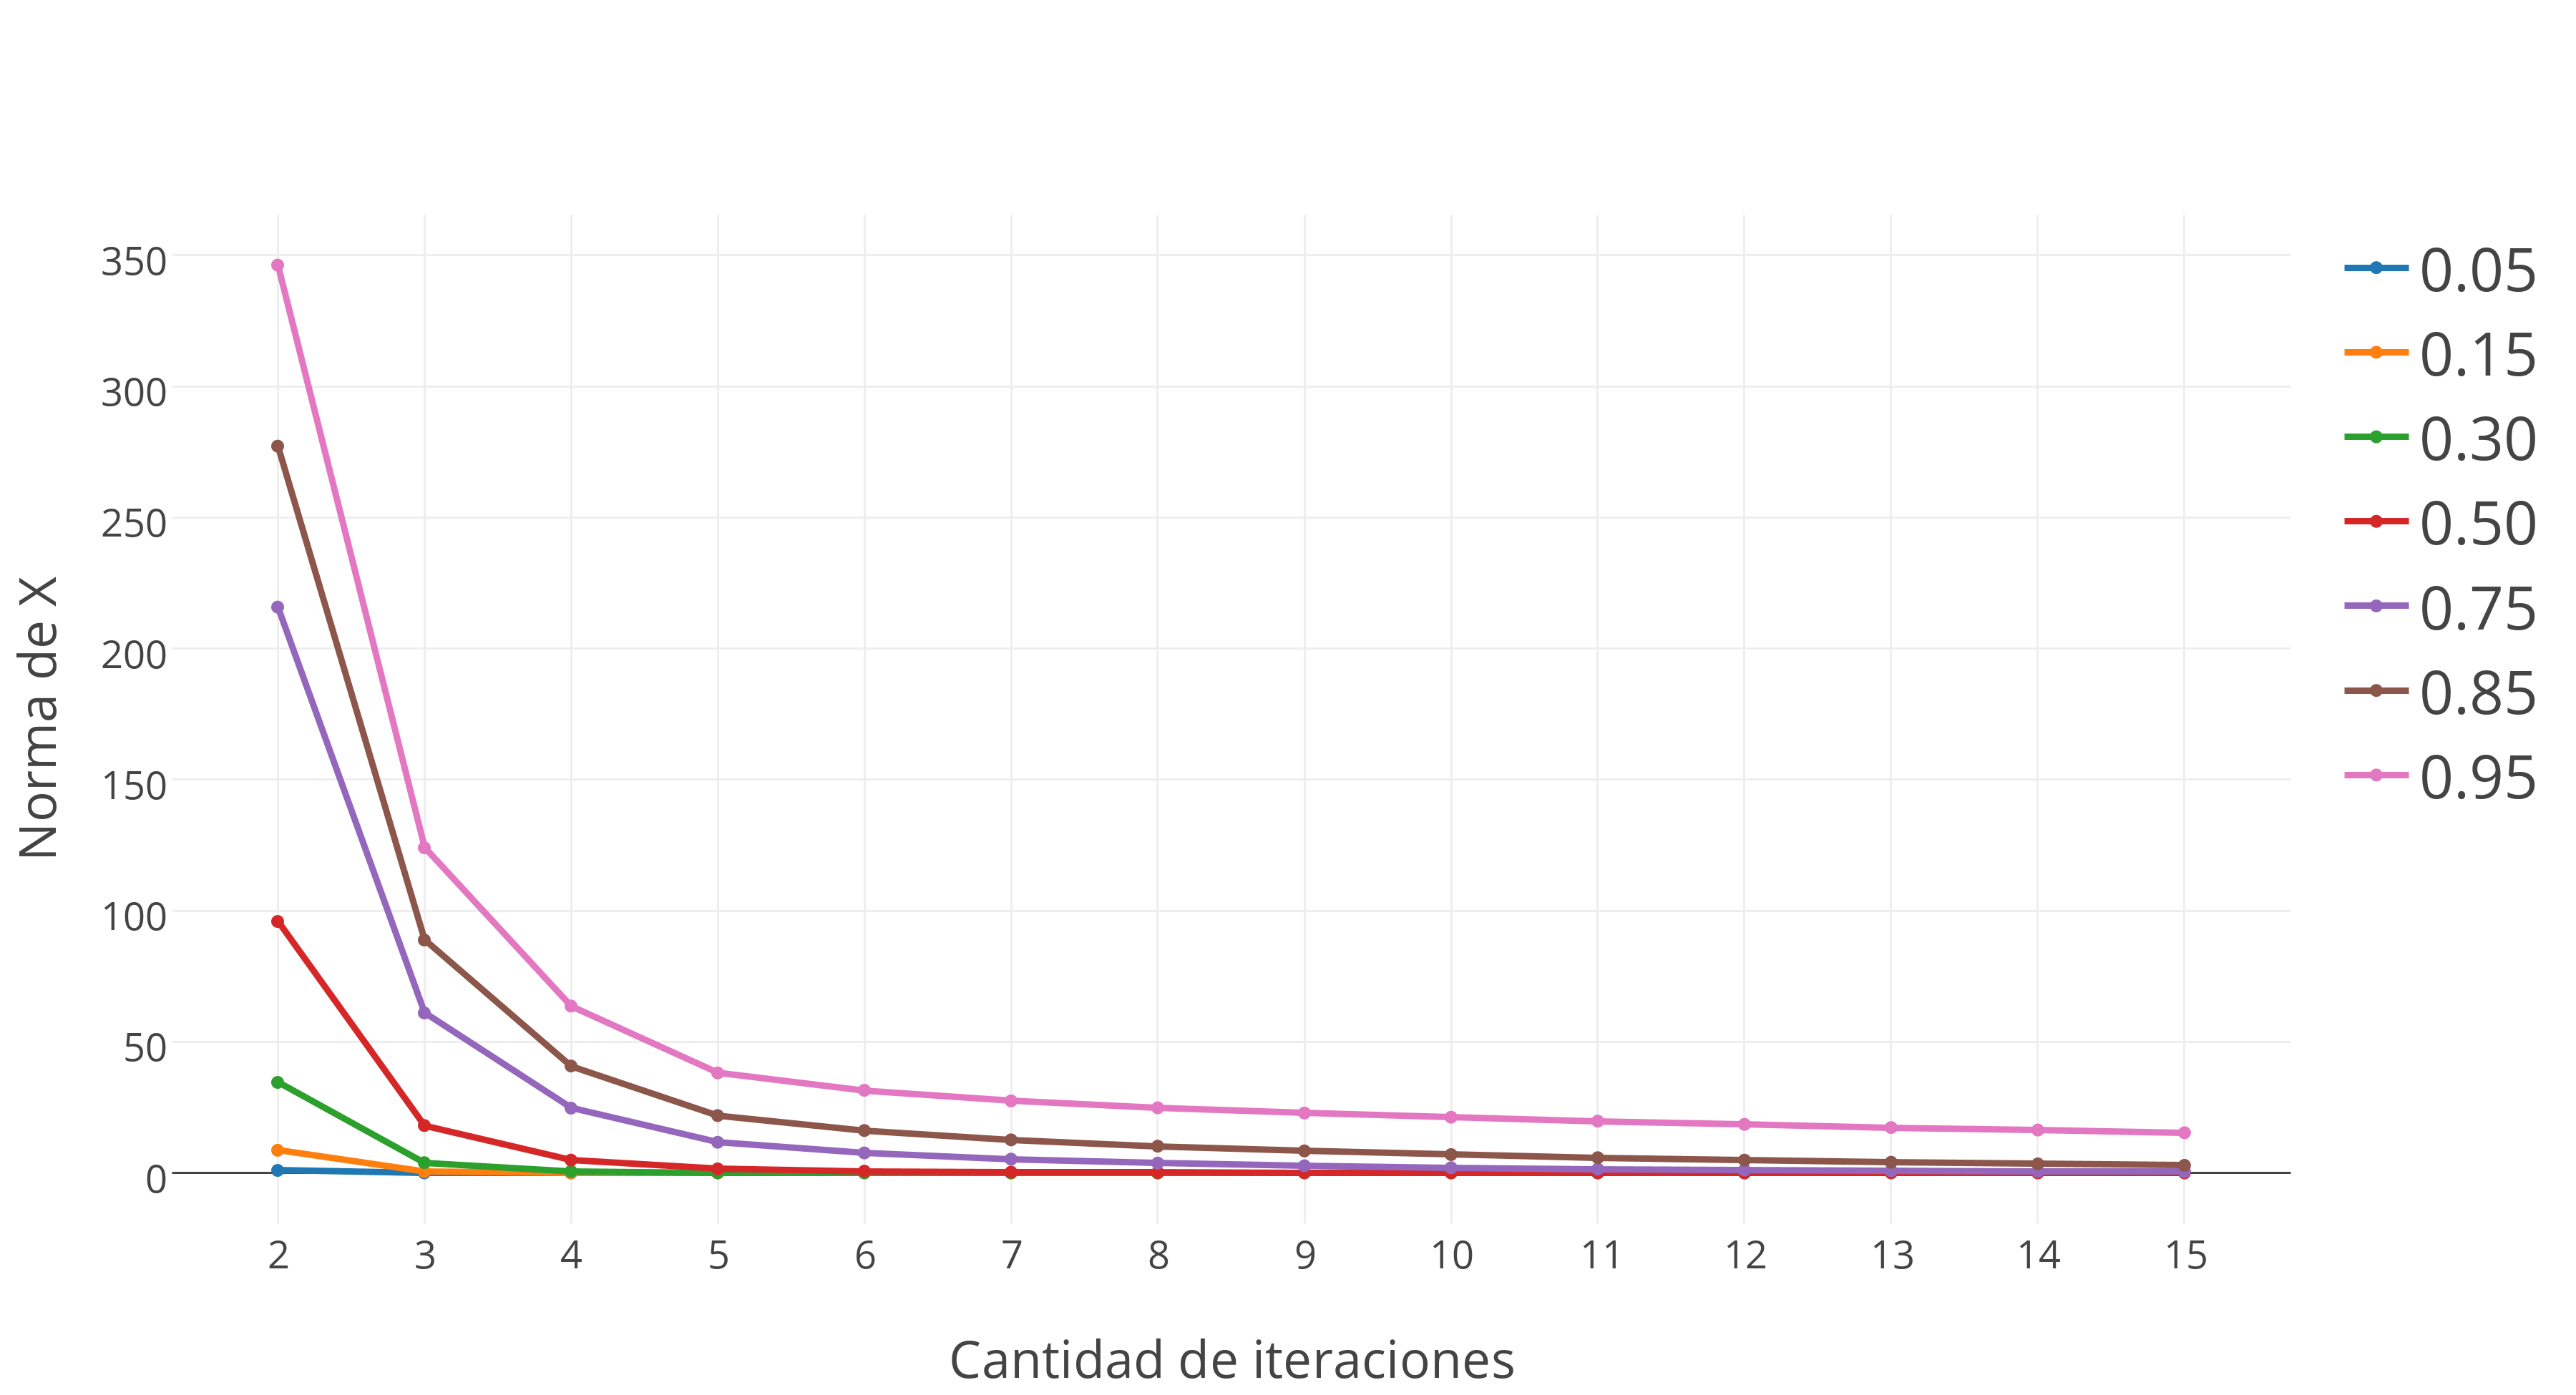
\includegraphics[scale=0.50]{imagenes/exp12/complexityPAGERANK.png}
	\caption{Variaci\'on de la norma cambiando el C para la Red Complexity}
	\label{nombreparareferenciar}
  \end{center}
\end{figure}
En la siguiente tabla se muestran la cantidad de iteraciones necesarias para distintos C bajo la misma Red: \\
 \begin{tabular}[c]{|c|c|c|c|c|c|c|c|}
\hline
 & C=0.05 & C=0.15 & C=0.30 & C=0.50 & C=0.75 & C=0.85 & C=0.95 \\
\hline
Cantidad &  & & & & & & \\ 
de Iteraciones & 5 & 8 & 12 & 21 & 49 & 86 & 268 \\
\hline
	\end{tabular}\\\\
\newpage


\begin{figure}[h!]
  \begin{center}
	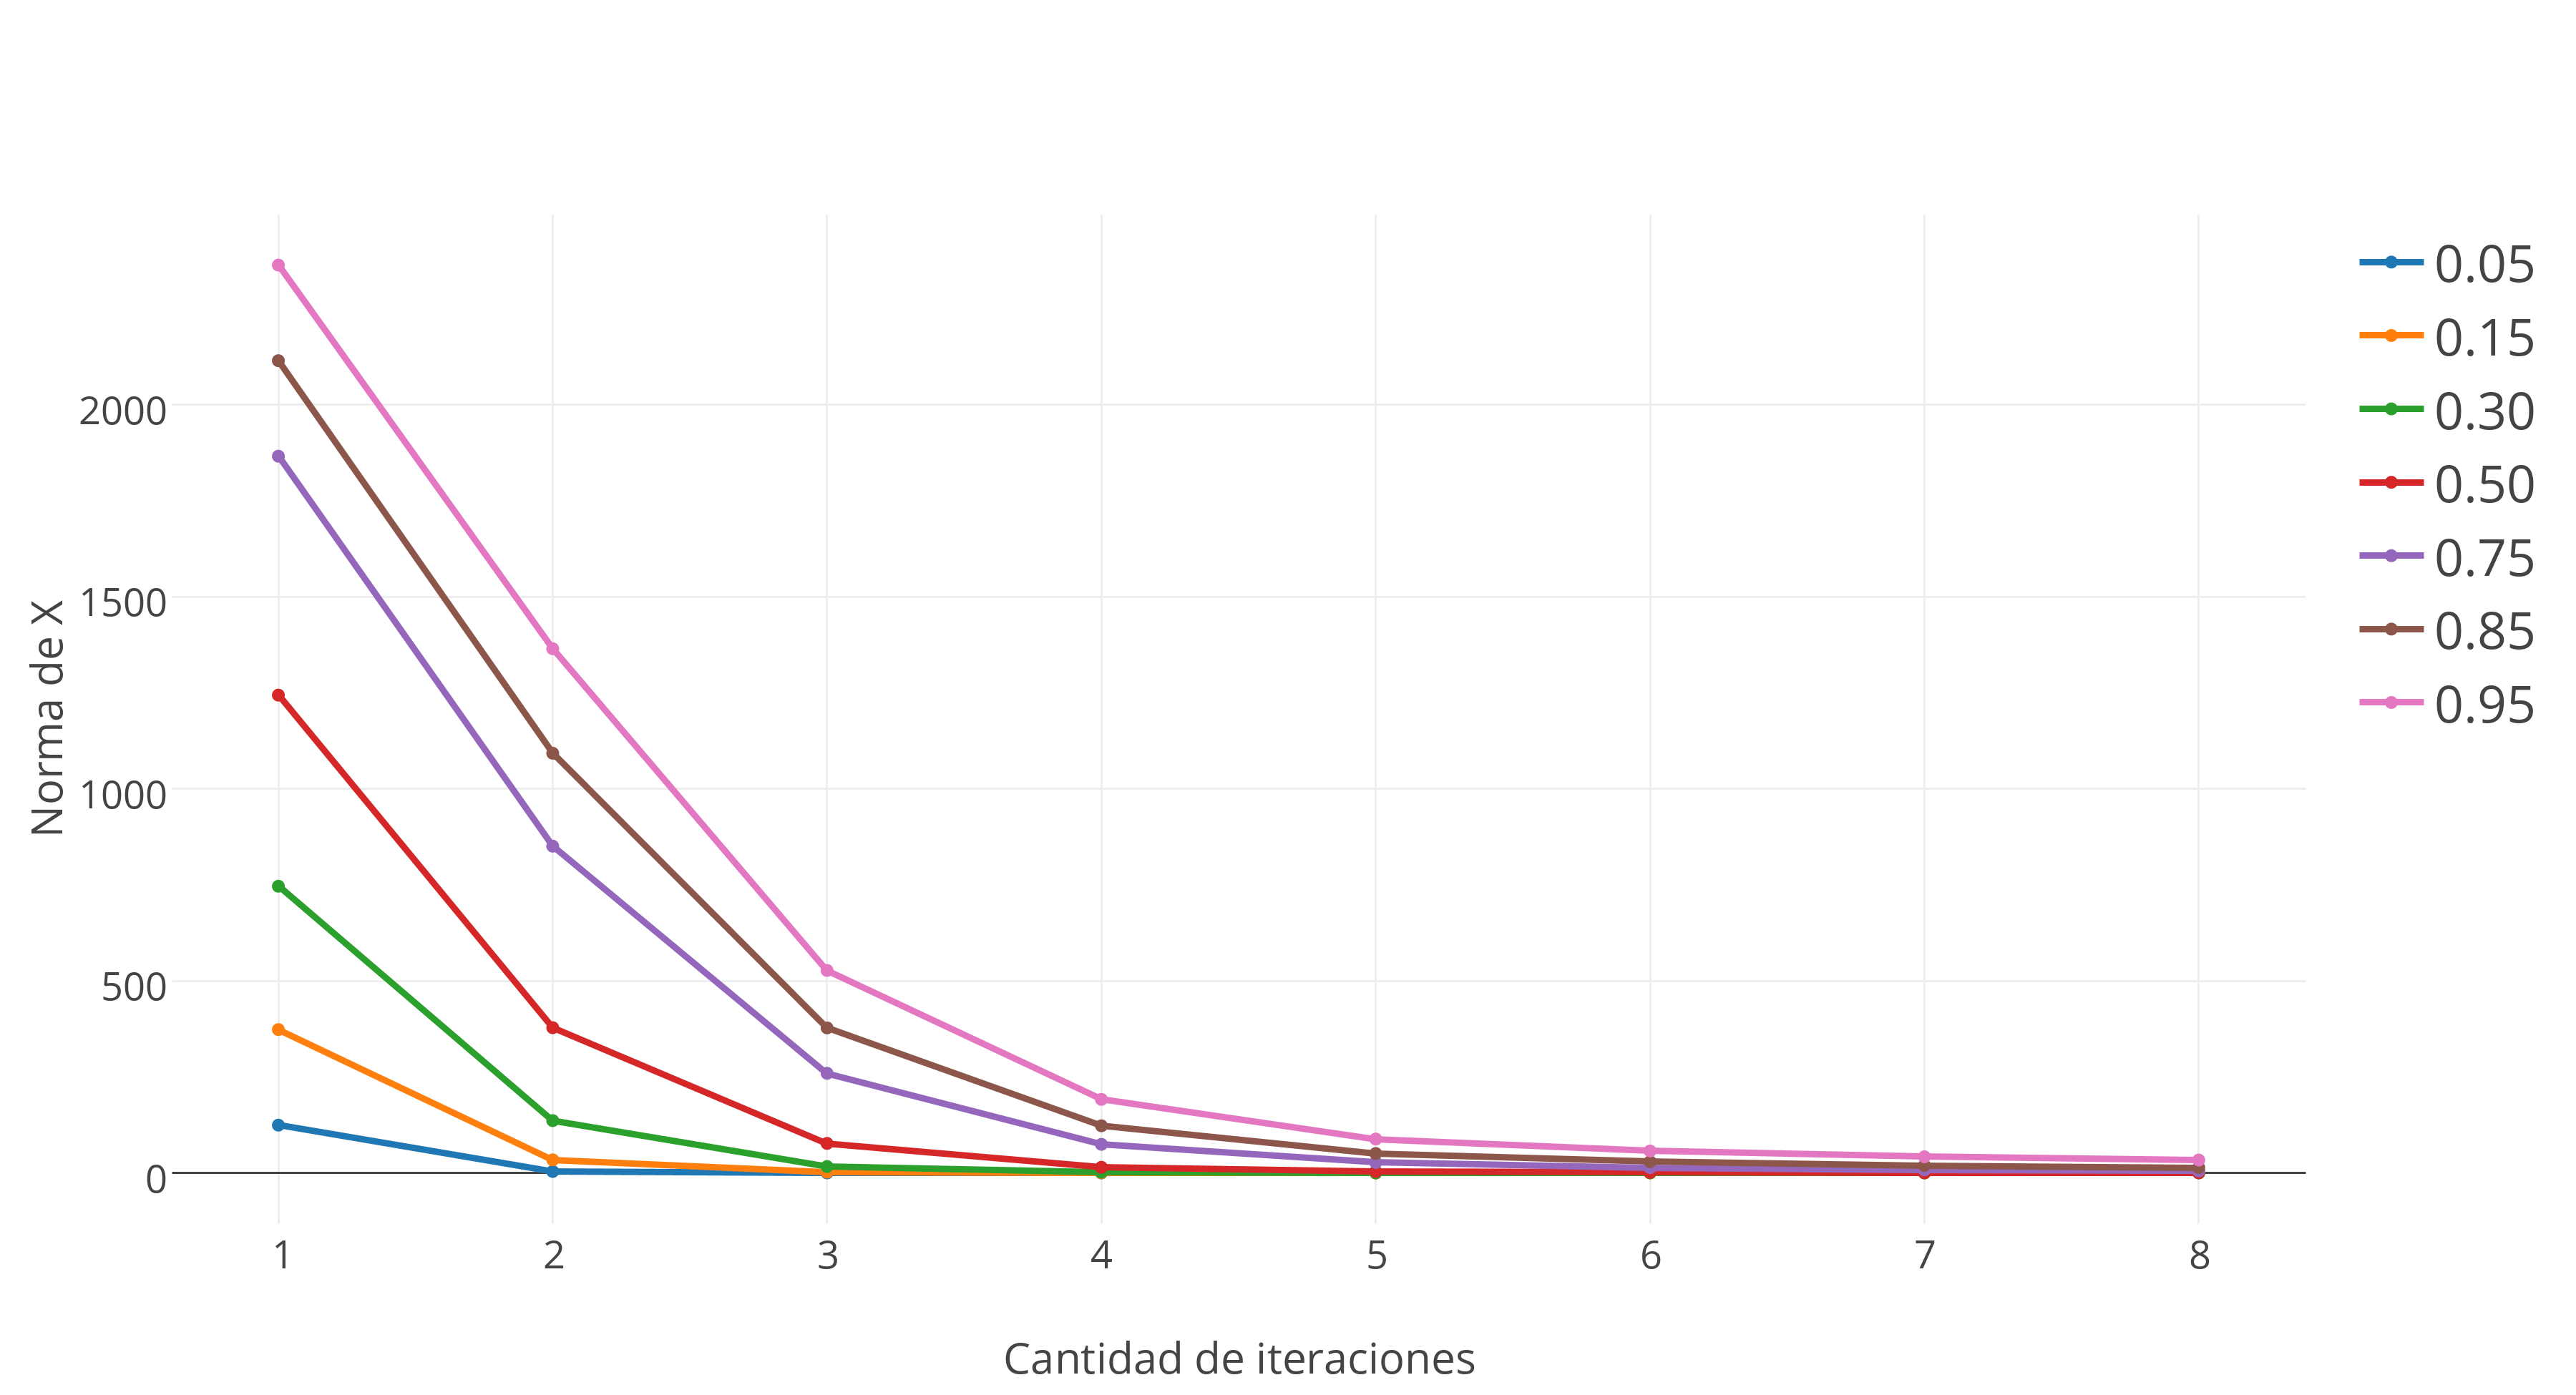
\includegraphics[scale=0.50]{imagenes/exp12/abortionPAGERANK.png}
	\caption{Variaci\'on de la norma cambiando el C para la Red Abortion}
	\label{nombreparareferenciar}
  \end{center}
\end{figure}
En la siguiente tabla se muestran la cantidad de iteraciones necesarias para distintos C bajo la misma Red: \\
 \begin{tabular}[c]{|c|c|c|c|c|c|c|c|}
\hline
 & C=0.05 & C=0.15 & C=0.30 & C=0.50 & C=0.75 & C=0.85 & C=0.95 \\
\hline
Cantidad &  & & & & & & \\ 
de Iteraciones & 5 & 7 & 11 & 19 & 46 & 80 & 251 \\
\hline
	\end{tabular}\\\\
\newpage


\begin{figure}[h!]
  \begin{center}
	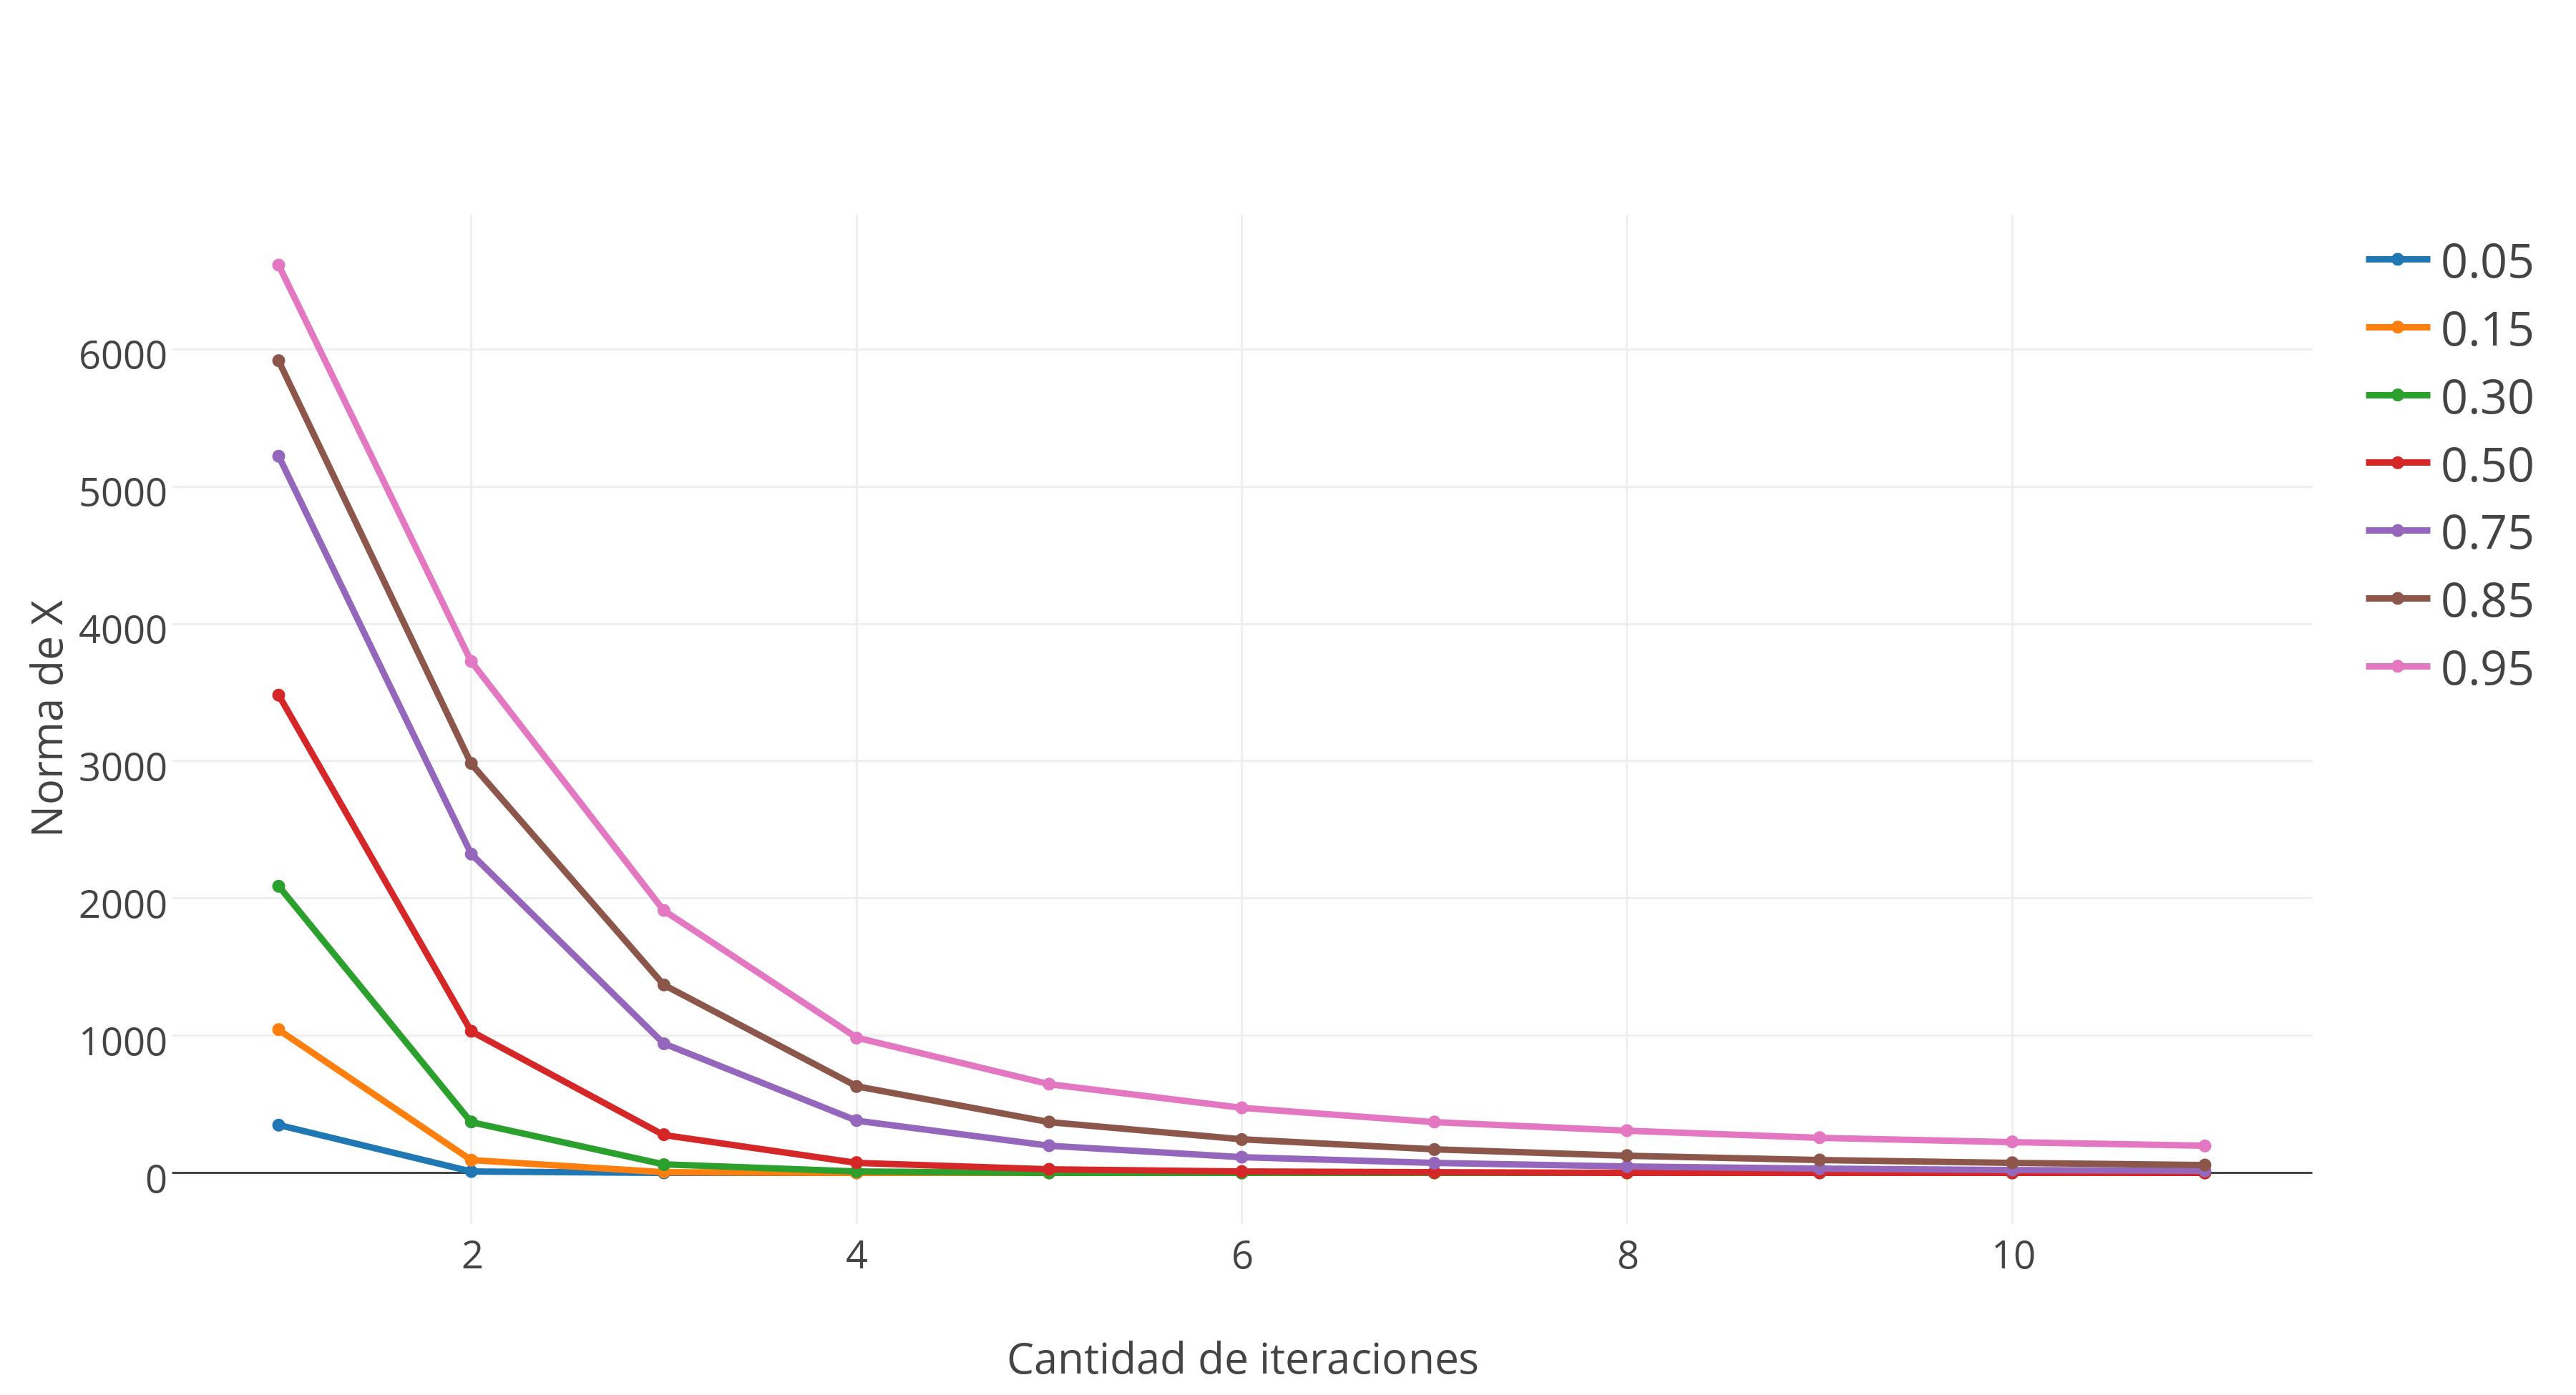
\includegraphics[scale=0.50]{imagenes/exp12/moviesPAGERANK.png}
	\caption{Variaci\'on de la norma cambiando el C para la Red Movies}
	\label{nombreparareferenciar}
  \end{center}
\end{figure}
En la siguiente tabla se muestran la cantidad de iteraciones necesarias para distintos C bajo la misma Red: \\
 \begin{tabular}[c]{|c|c|c|c|c|c|c|c|}
\hline
& C=0.05 & C=0.15 & C=0.30 & C=0.50 & C=0.75 & C=0.85 & C=0.95 \\
\hline
Cantidad &  & & & & & & \\ 
de Iteraciones & 6 & 8 & 13 & 21 & 51 & 90 & 282 \\
\hline
	\end{tabular}\\\\
\\

\begin{figure}[h!]
  \begin{center}
	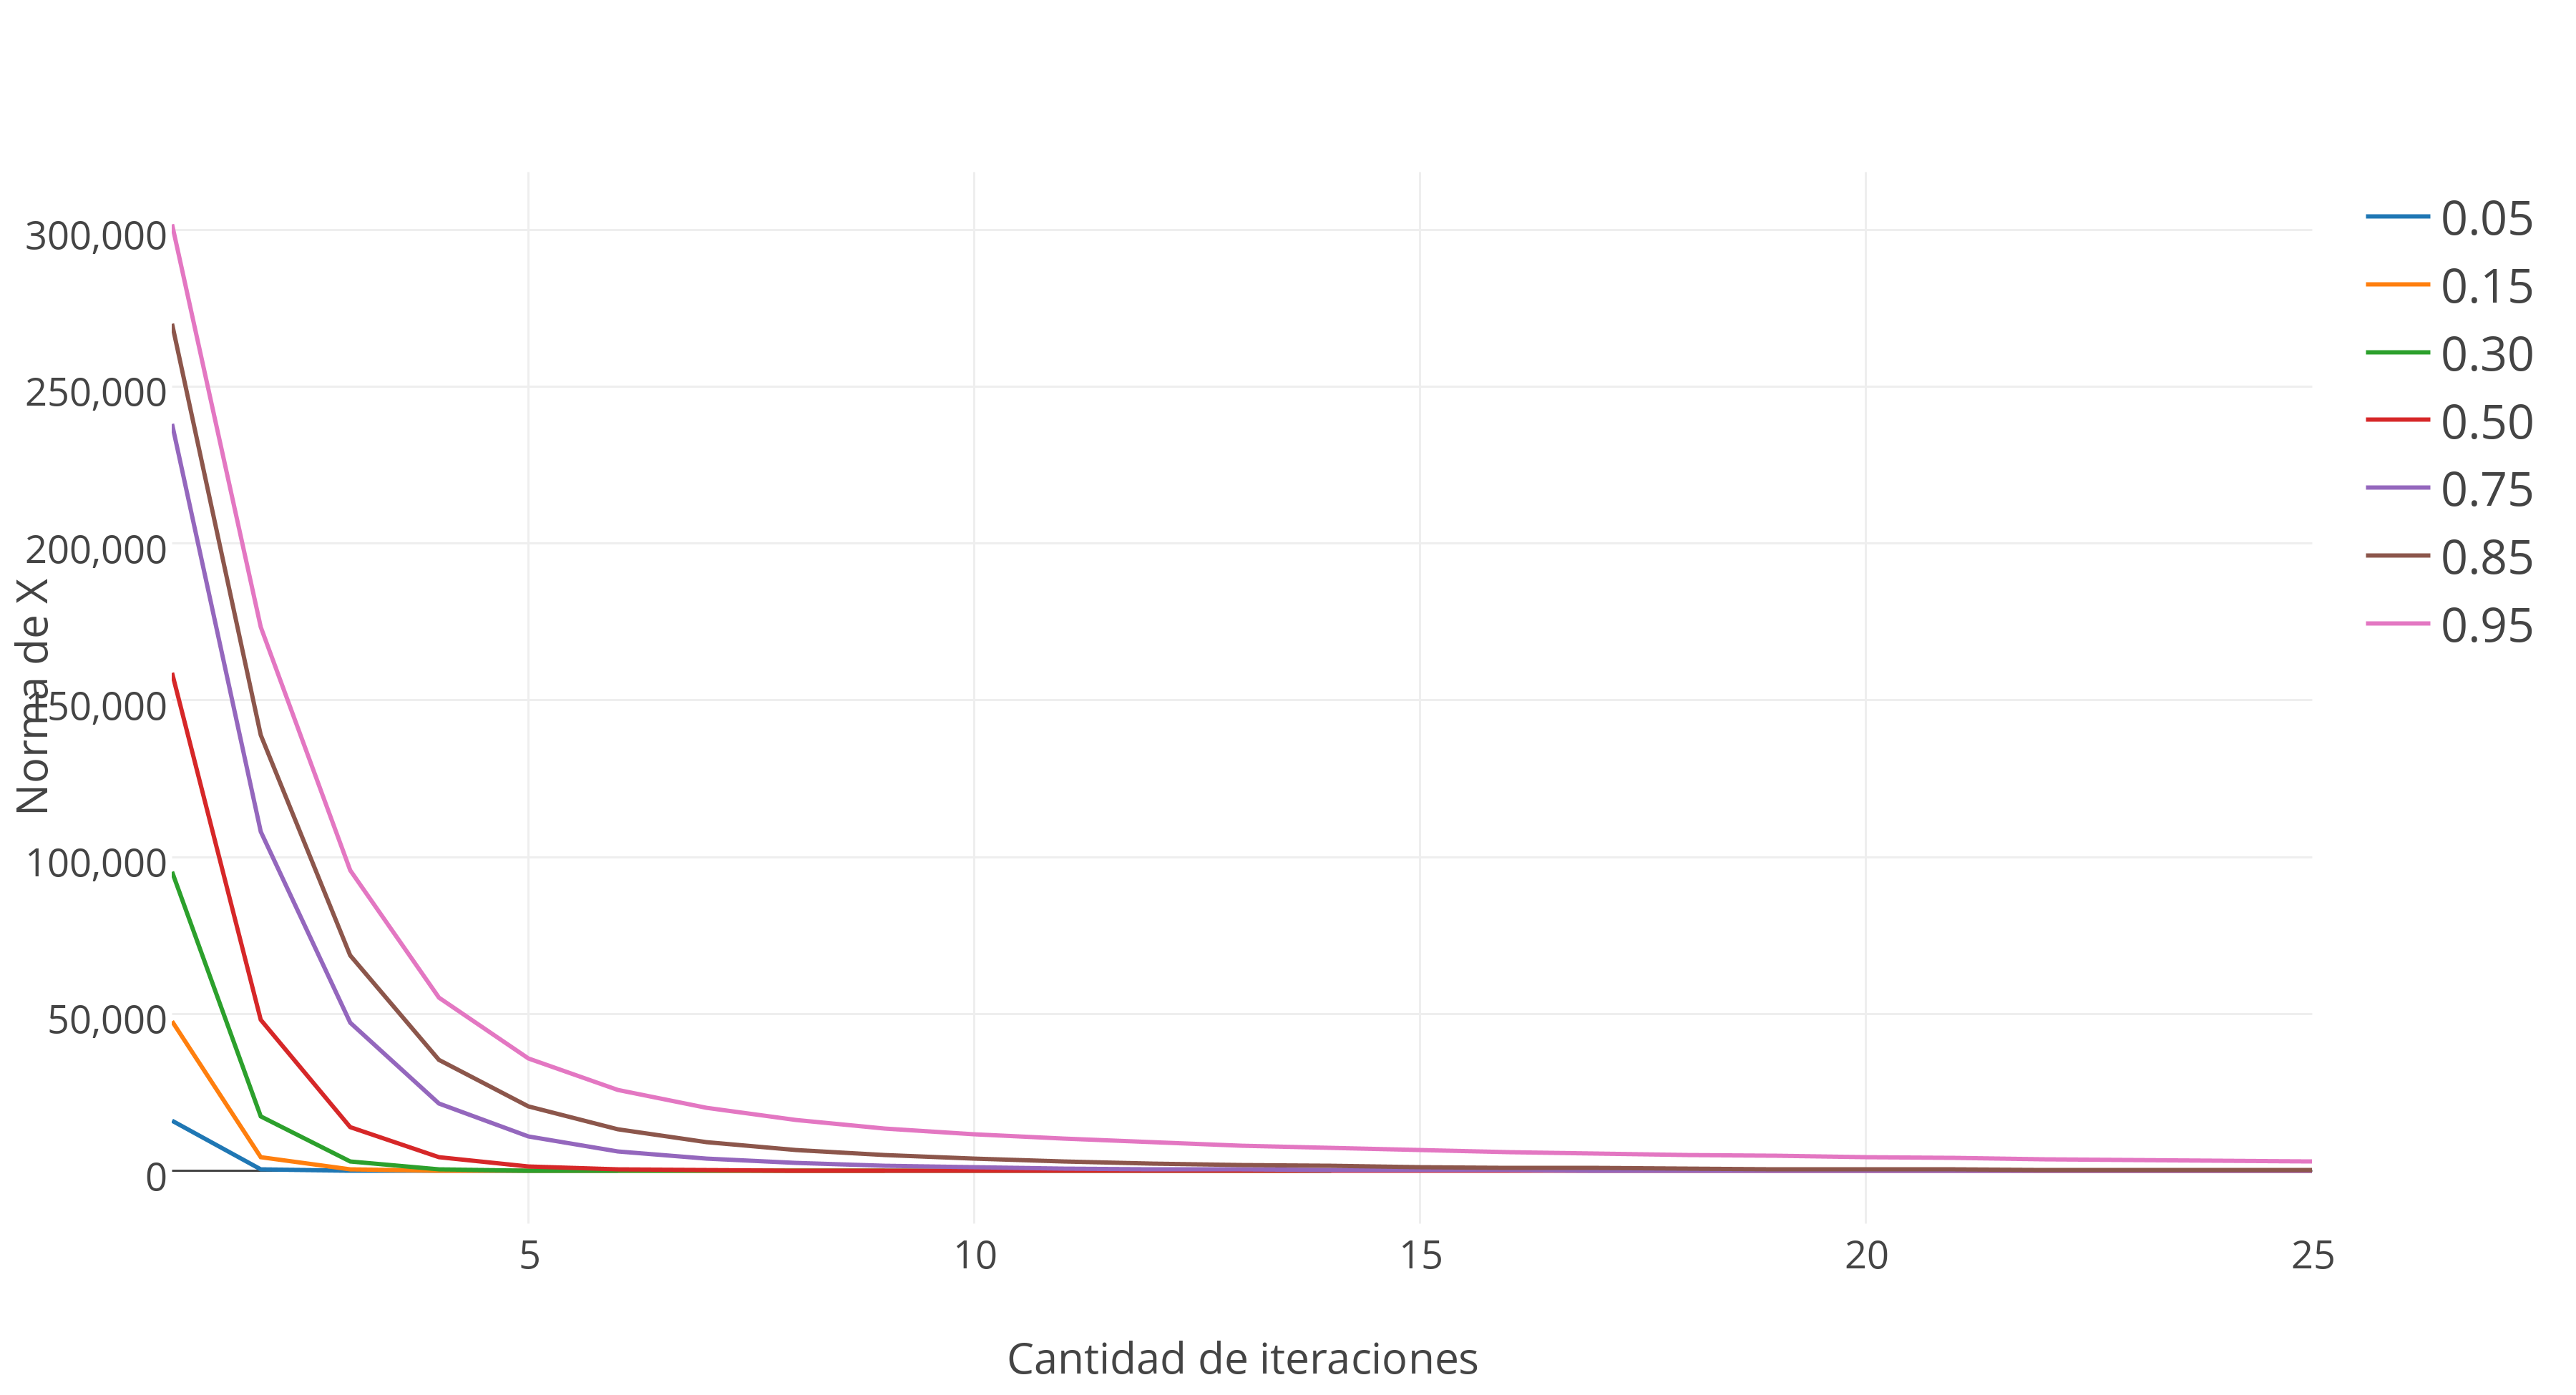
\includegraphics[scale=0.50]{imagenes/exp12/stanfordPAGERANK.png}
	\caption{Variaci\'on de la norma cambiando el C para la Red Stanford}
	\label{nombreparareferenciar}
  \end{center}
\end{figure}

En la siguiente tabla se muestran la cantidad de iteraciones necesarias para distintos C bajo la misma Red: \\
 \begin{tabular}[c]{|c|c|c|c|c|c|c|c|}
\hline
 & C=0.05 & C=0.15 & C=0.30 & C=0.50 & C=0.75 & C=0.85 & C=0.95 \\
\hline
Cantidad &  & & & & & & \\ 
de Iteraciones & 6 & 9 & 14 & 25 & 59 & 104 & 329\\
\hline
	\end{tabular}\\\\	
\\	
\begin{figure}[h!]
  \begin{center}
	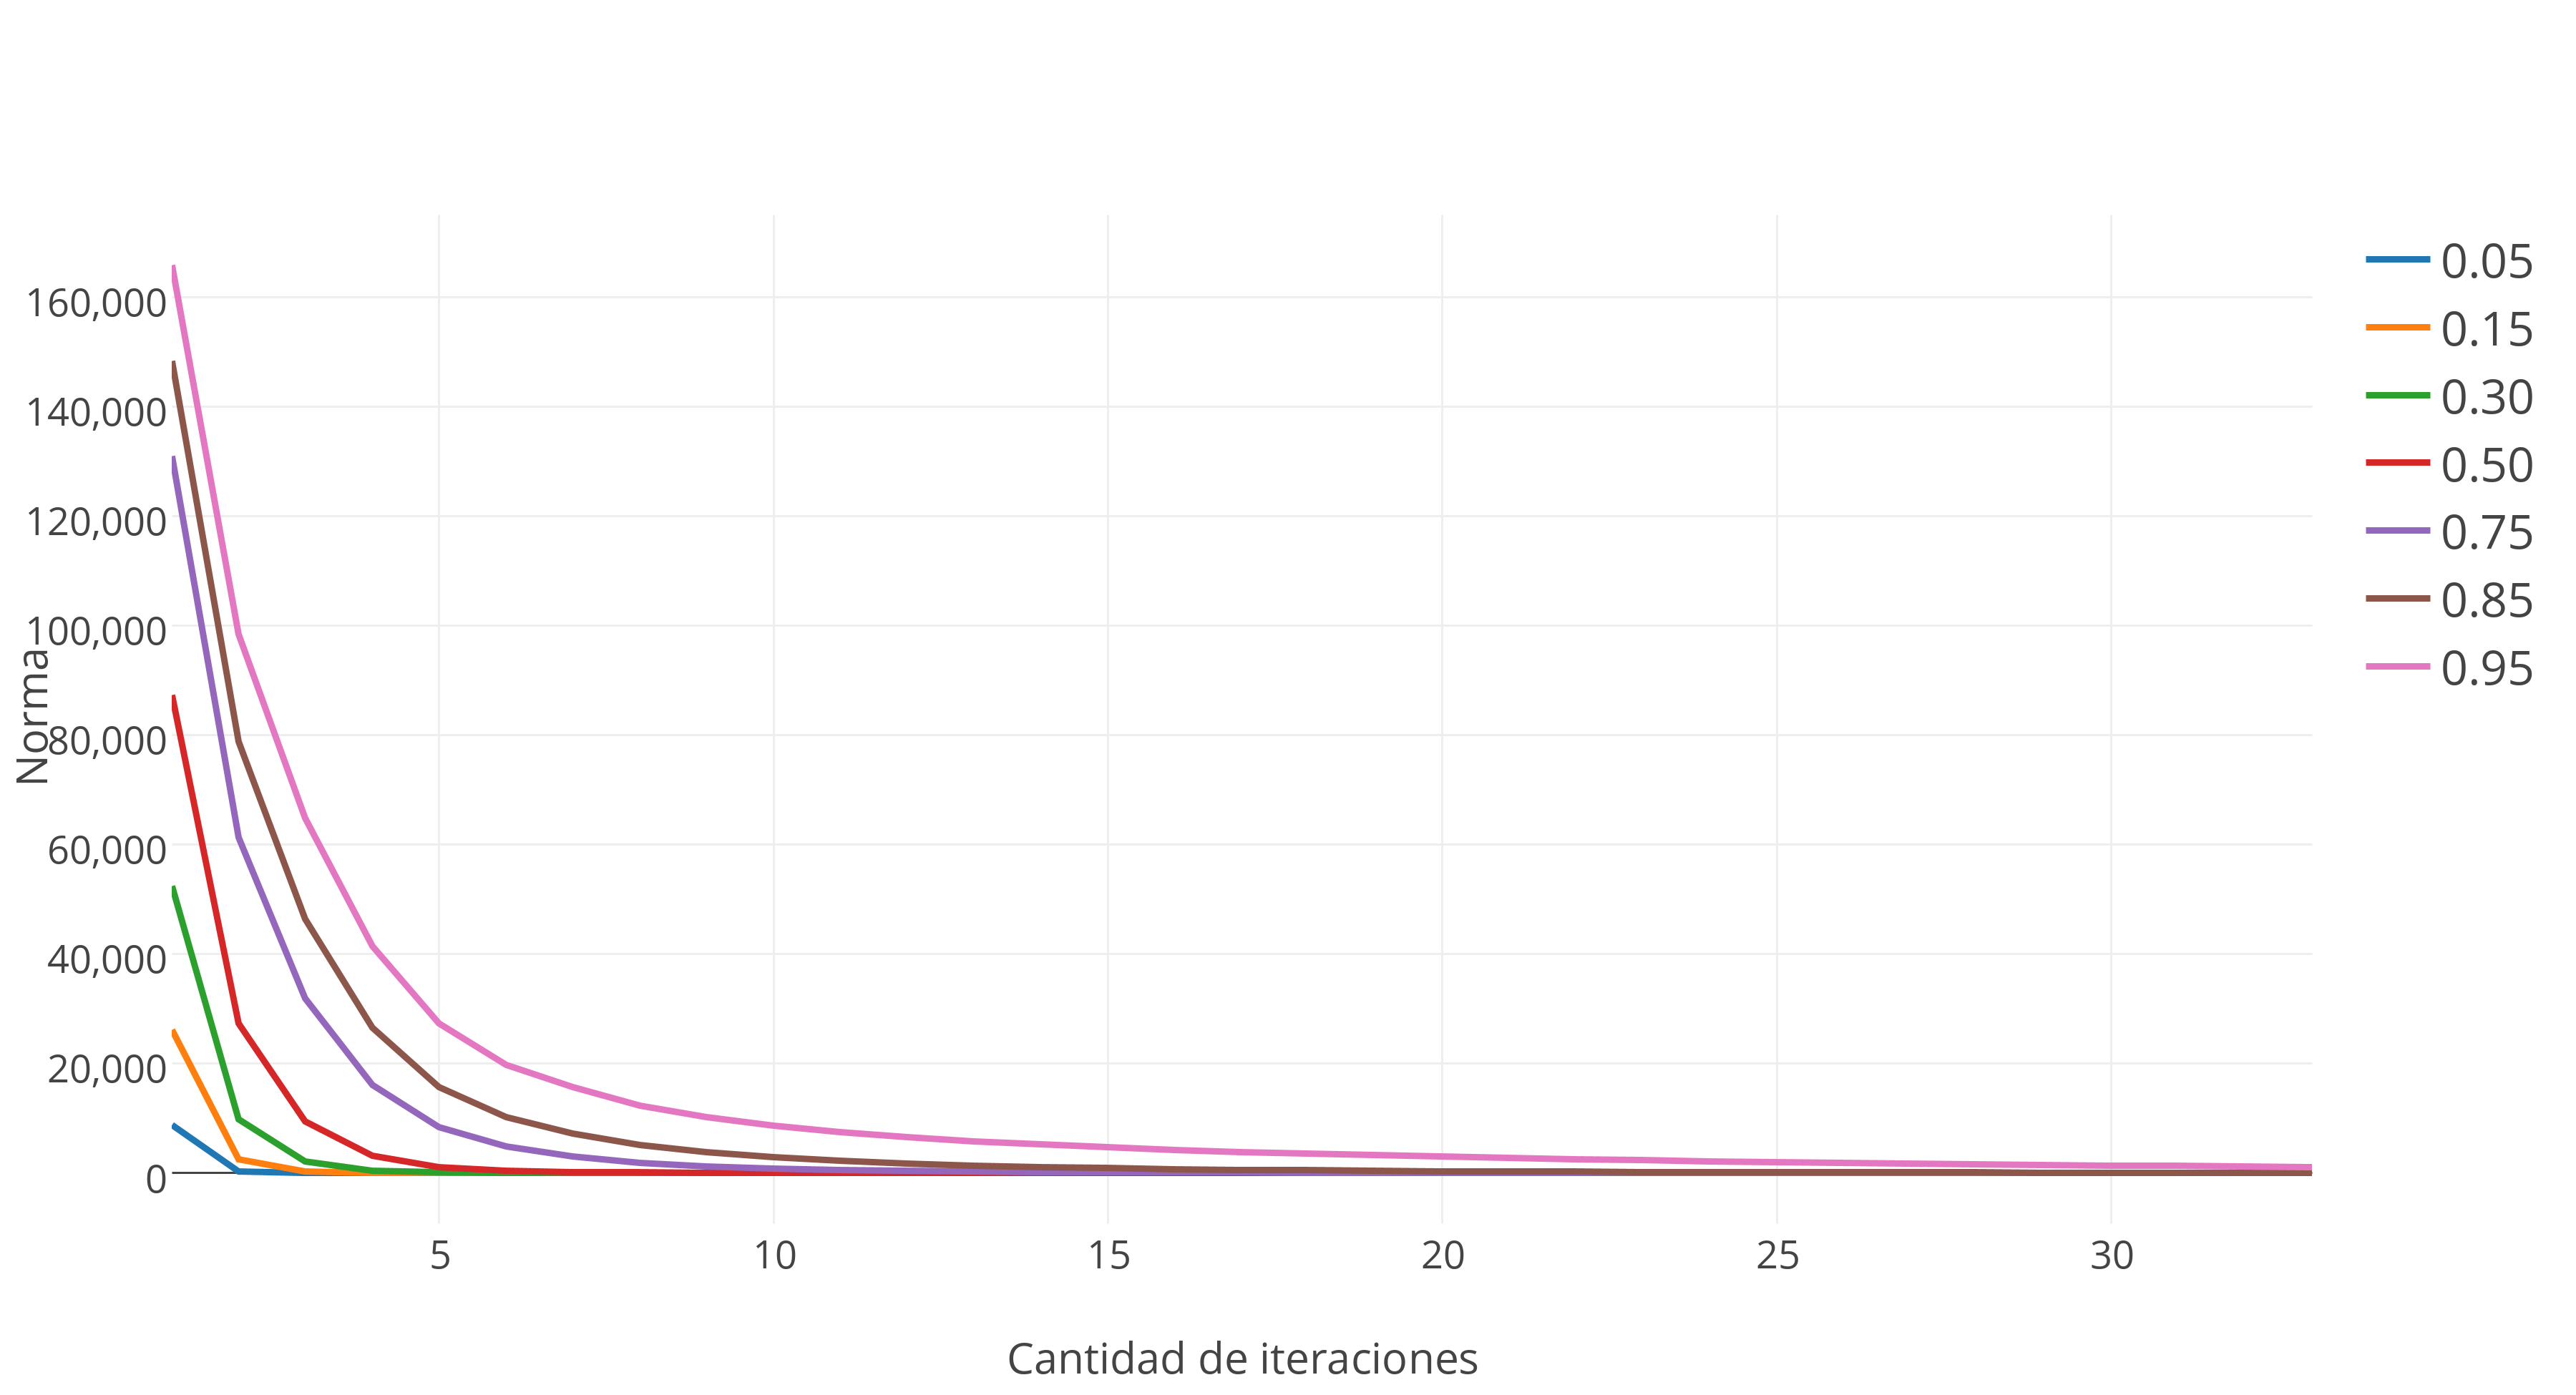
\includegraphics[scale=0.50]{imagenes/exp12/notredamePAGERANK.png}
	\caption{Variaci\'on de la norma cambiando el C para la Red Notre Dame}
	\label{nombreparareferenciar}
  \end{center}
\end{figure}
En la siguiente tabla se muestran la cantidad de iteraciones necesarias para distintos C bajo la misma Red: \\
 \begin{tabular}[c]{|c|c|c|c|c|c|c|c|}
\hline
 & C=0.05 & C=0.15 & C=0.30 & C=0.50 & C=0.75 & C=0.85 & C=0.95 \\
\hline
Cantidad &  & & & & & & \\ 
de Iteraciones & 6 & 10 & 15 & 25 & 56 & 96 & 295\\
\hline
	\end{tabular}\\\\
\\
\\
\indent Experimentamos con Redes de distintos tama\~nos y podemos afimar que para todas ellas: \emph{Cuanto mayor es el C, se necesita una mayor cantidad de iteraciones para concluir algor\'itmicamente que ya convergi\'o el vector $x$ a $x\ast$}. Es decir, que se aumenta la cantidad de veces que se ejecuta el ciclo hasta que la norma de la diferencia entre X-actual y X-anterior sea menor a la tolerancia. Lo cual confirma nuestra hip\'otesis.
\newpage

\subsection{Convergencia de HITS}

\textbf{Hip\'otesis:} Nuestro planteo es que la norma 1 de la diferencia entre dos iteraciones consecutivas sobre el vector X y el vector Y va a converger al valor 0.\\
\\
\indent Esta idea surge de que el algoritmo implementado por HITS sea circular, es decir para actualizar los valores del vector X se utilizan los valores de Y y viceverssa. Por este motivo, se podr\'ia decir que se ``trasladan'' los pesos de X e Y al multiplicar cada vector por la matriz, y como en cada iteraci\'on se normalizan los vectores esto lleva a que los valores a trabajar sean menores de iteraci\'on a iteraci\'on. \\
\\


Los siguientes gr\'aficos est\'an citados en orden creciente de tama\~no de las redes:\\


\begin{figure}[h!]
  \begin{center}
	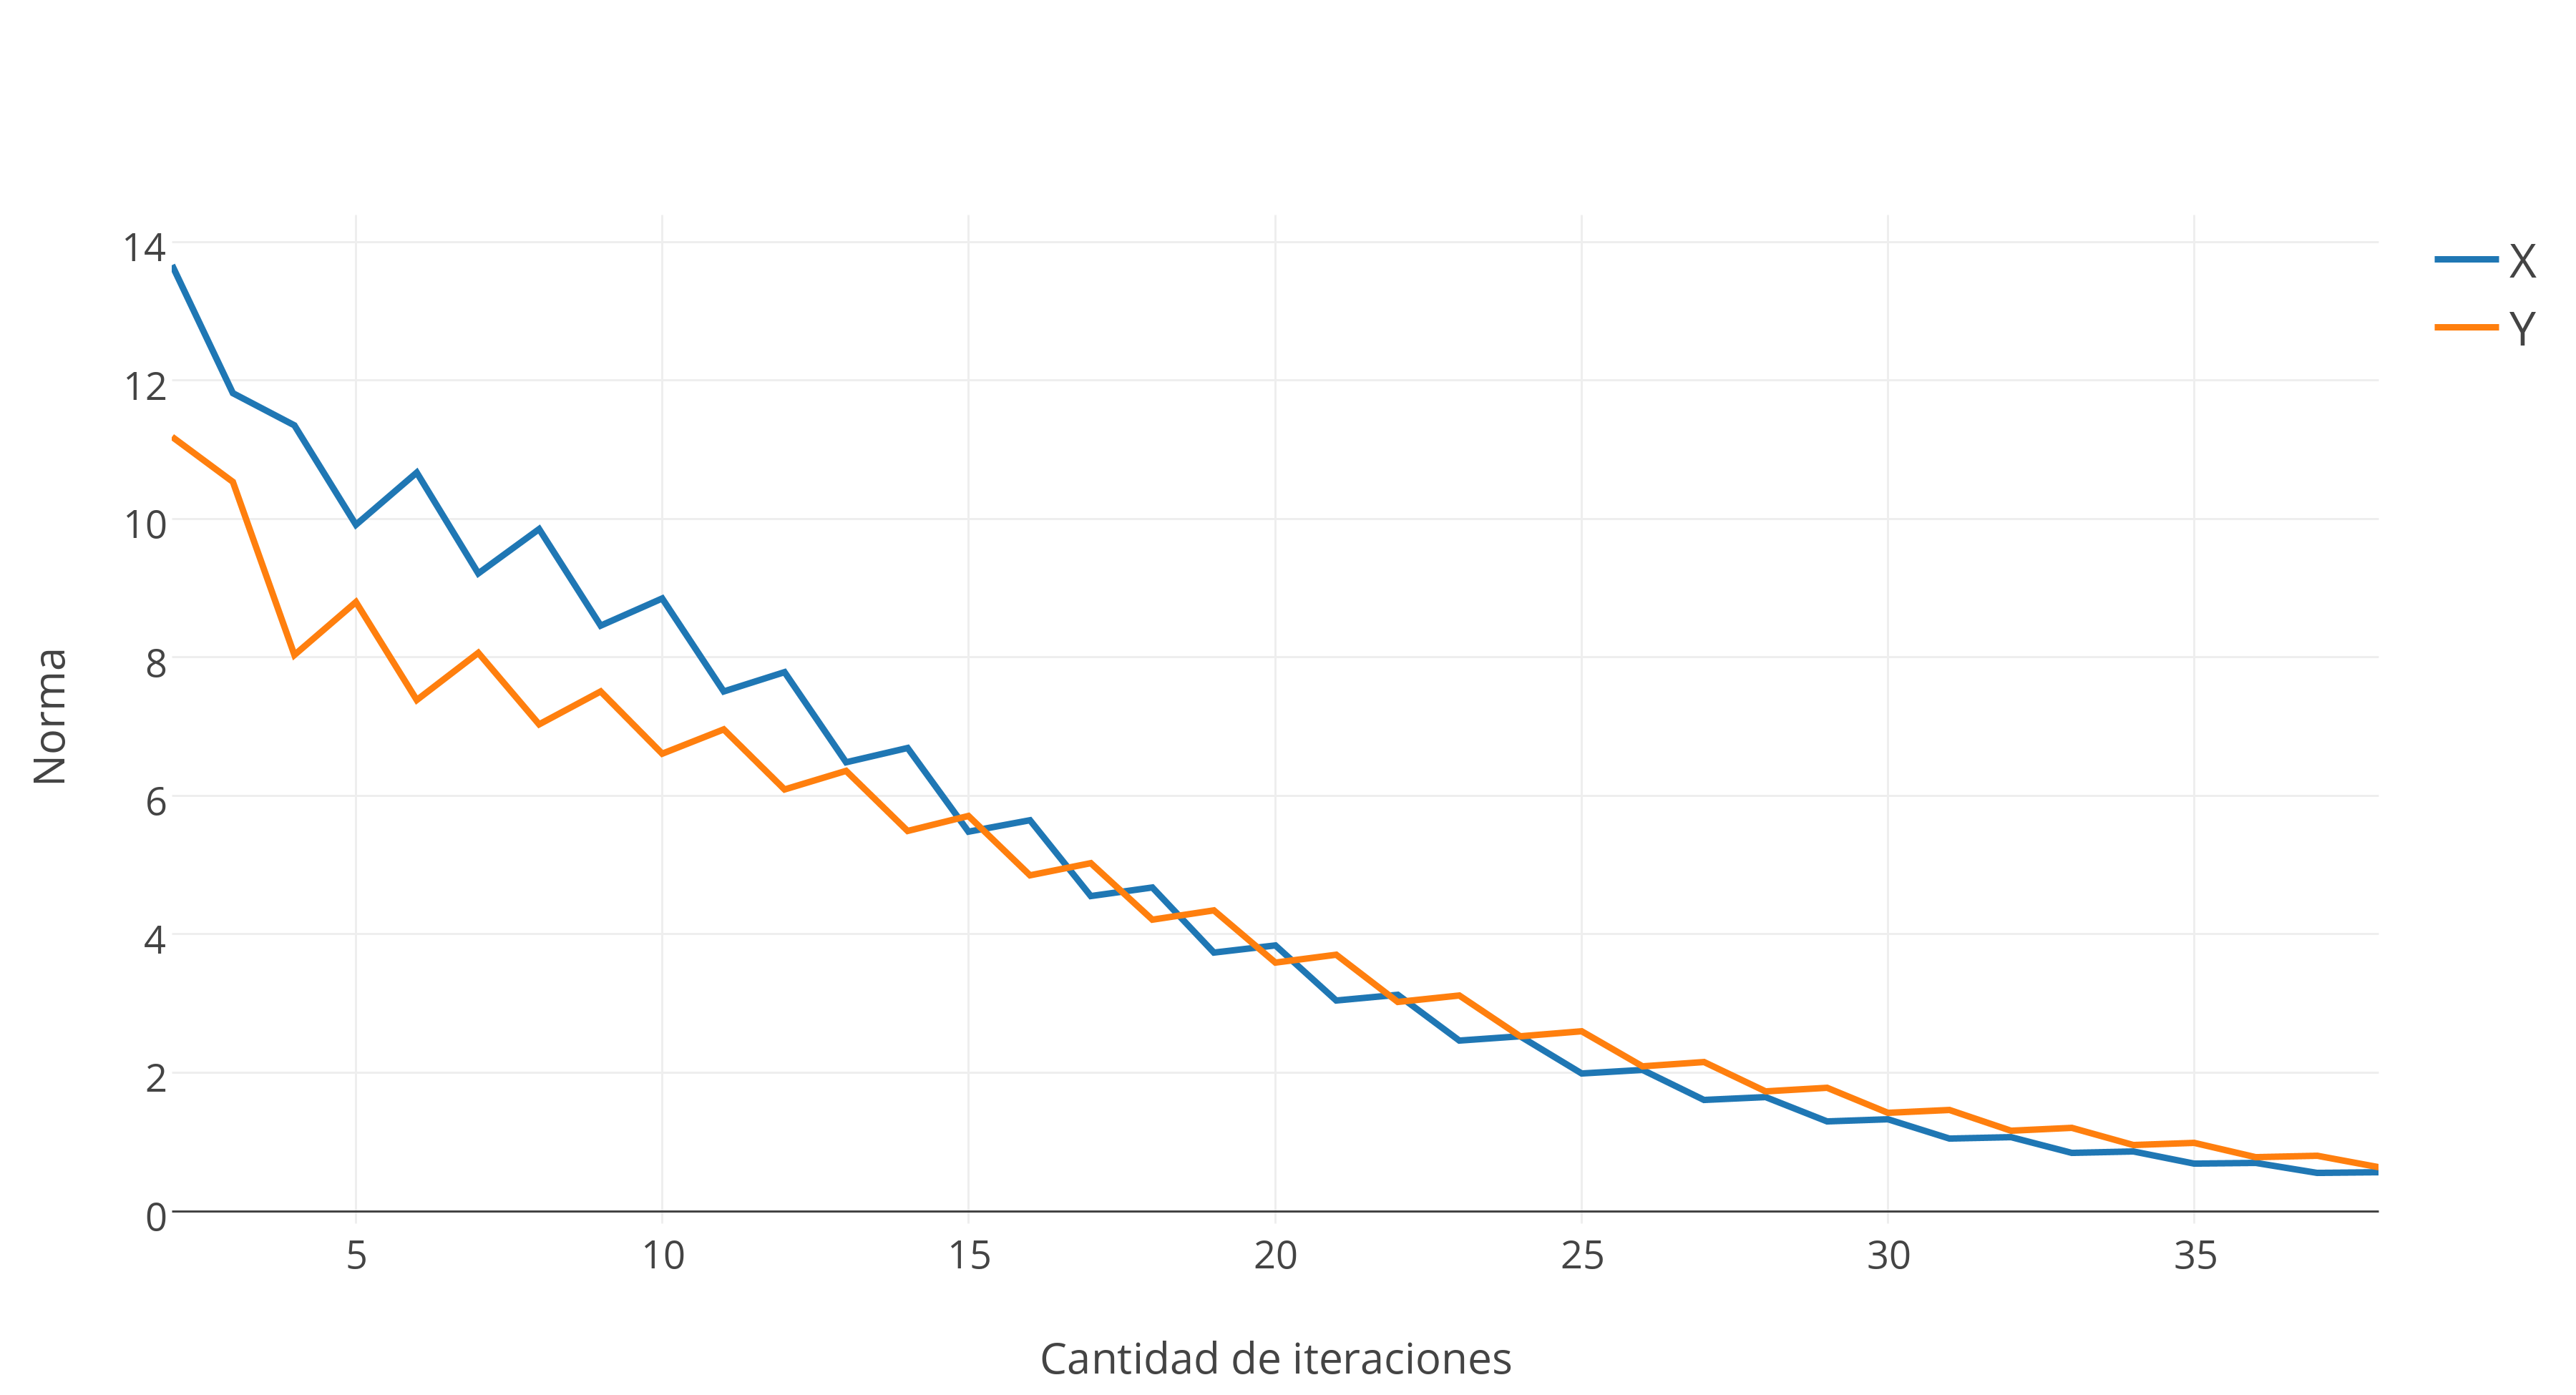
\includegraphics[scale=0.50]{imagenes/exp12/complexityHITS.png}
	\caption{Variaci\'on de la norma de X e Y en cada iteraci\'on para la Red Complexity}
	\label{nombreparareferenciar}
	\textit{La cantidad de iteraciones llevadas a cabo por el algoritmo fue de 121.}
  \end{center}
\end{figure}
\newpage
\begin{figure}[h!]
  \begin{center}
	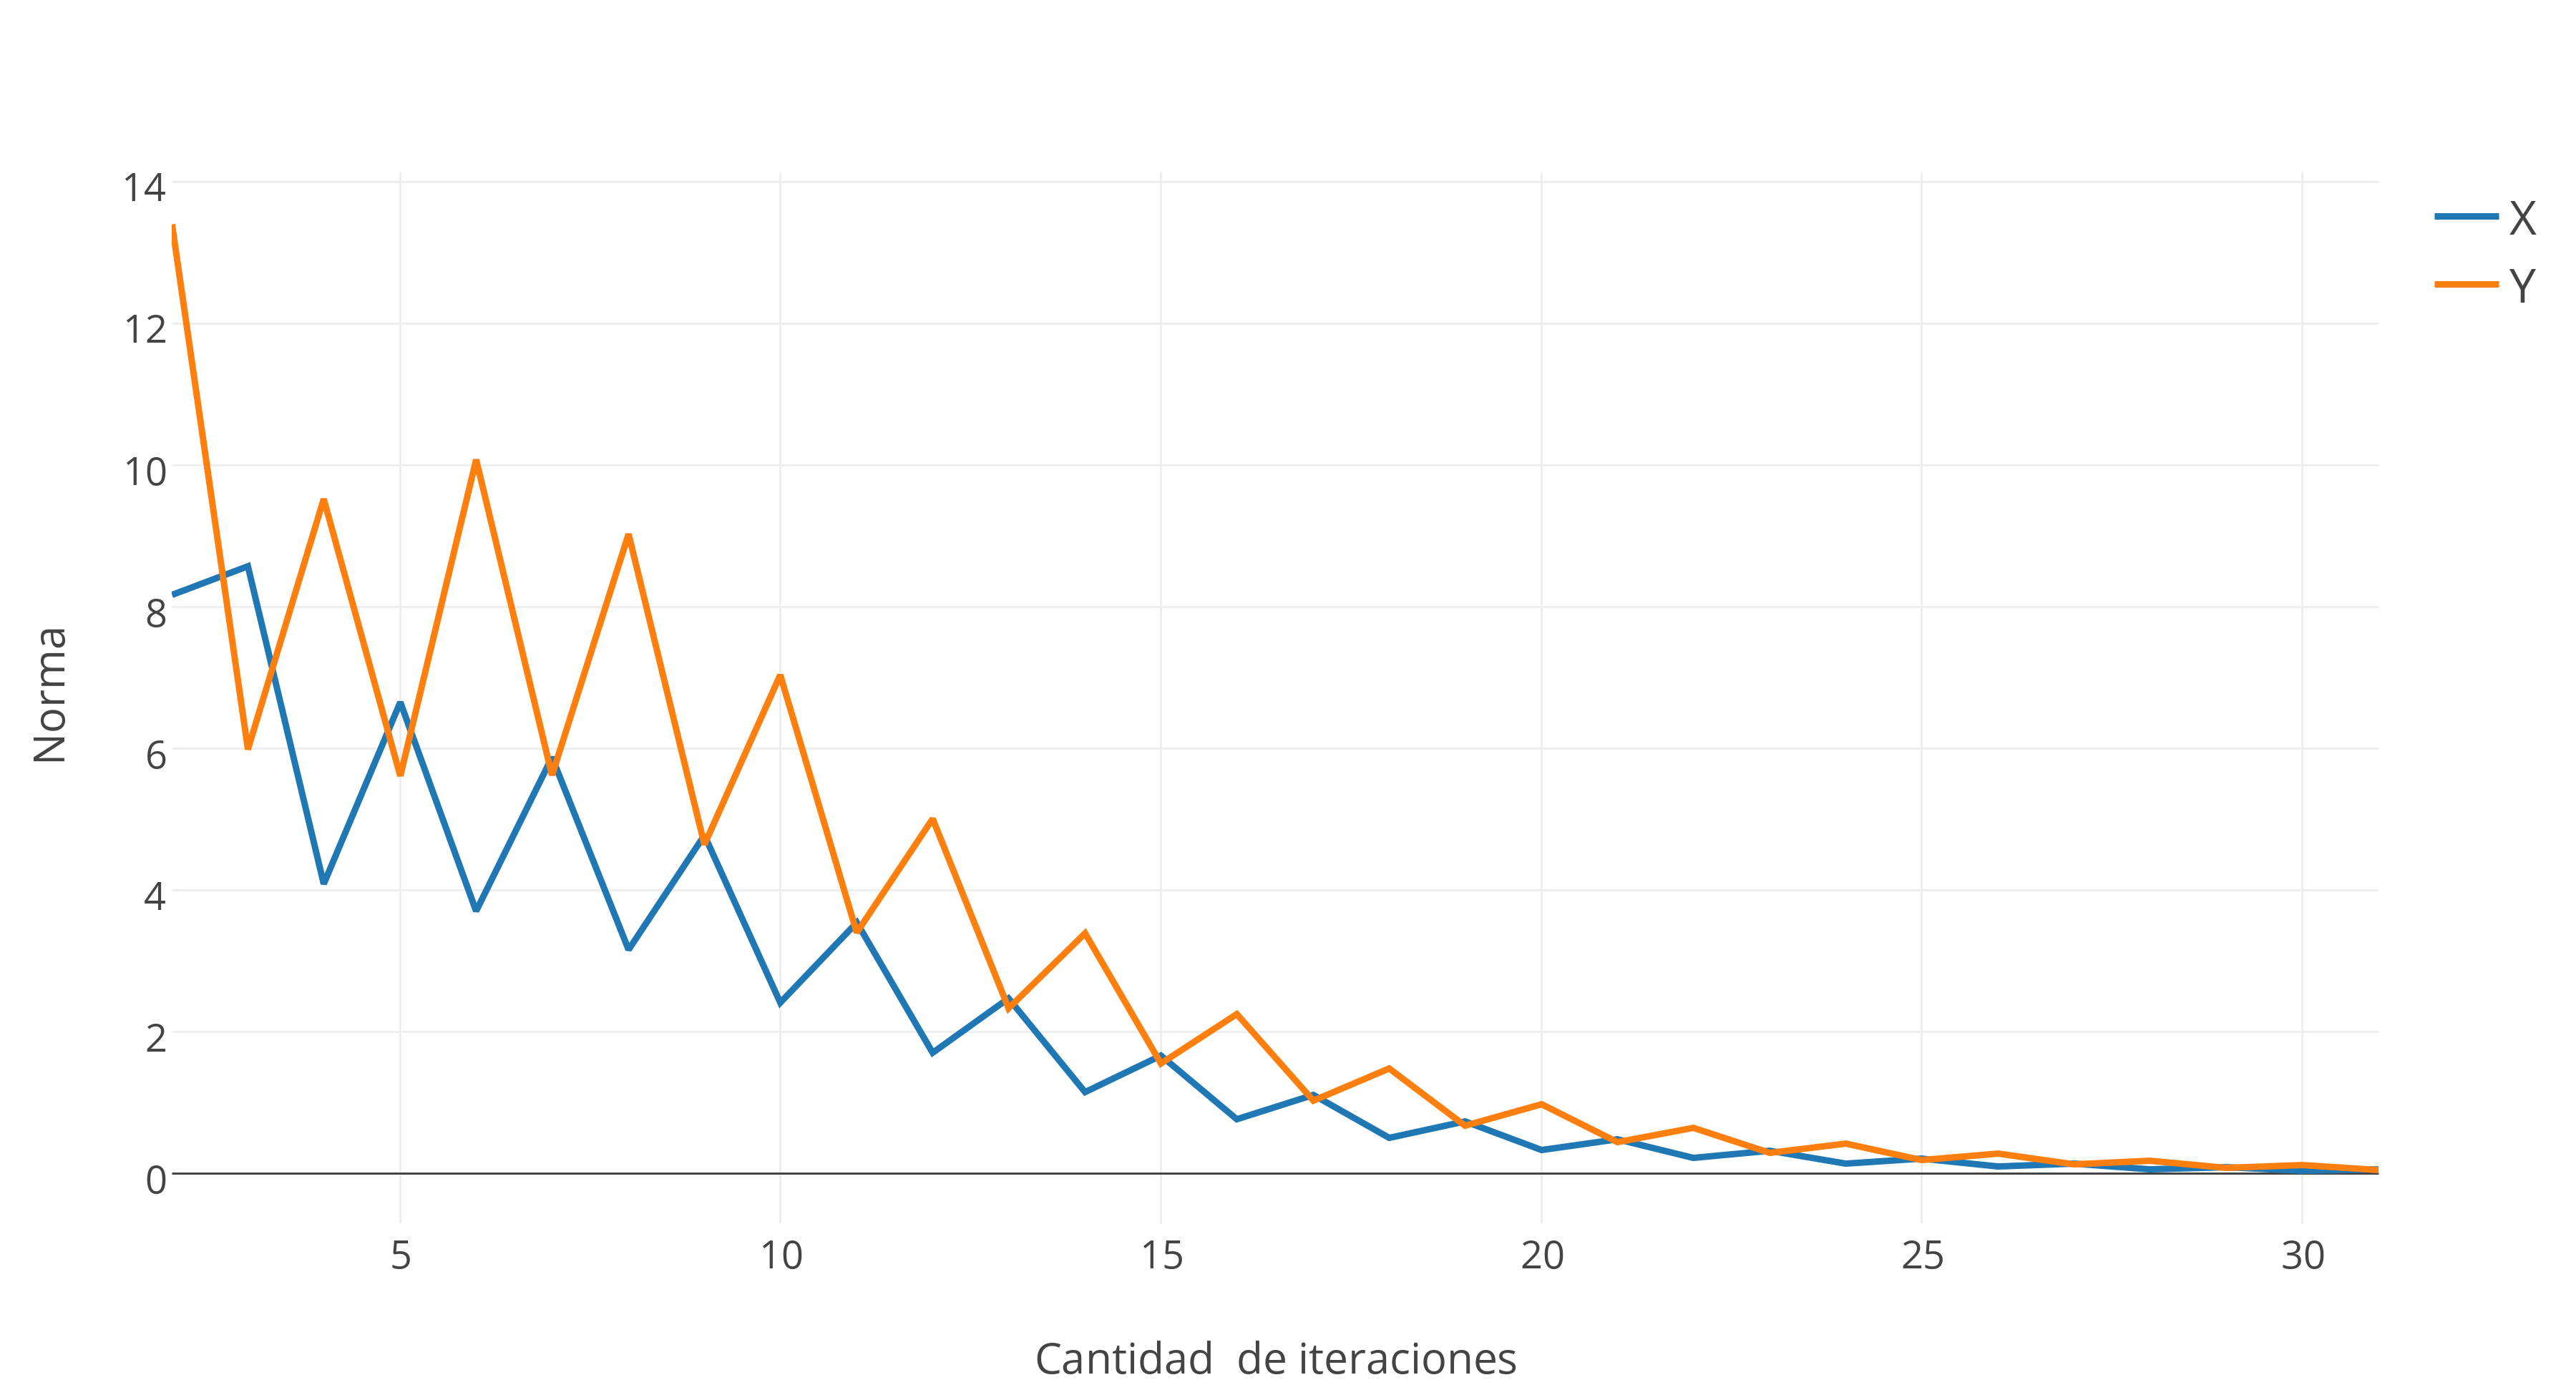
\includegraphics[scale=0.50]{imagenes/exp12/abortionHITS.png}
	\caption{Variaci\'on de la norma de X e Y en cada iteraci\'on para la Red Abortion}
	\label{nombreparareferenciar}
	\textit{La cantidad de iteraciones llevadas a cabo por el algoritmo fue de 56.}
  \end{center}
\end{figure}

\begin{figure}[h!]
  \begin{center}
	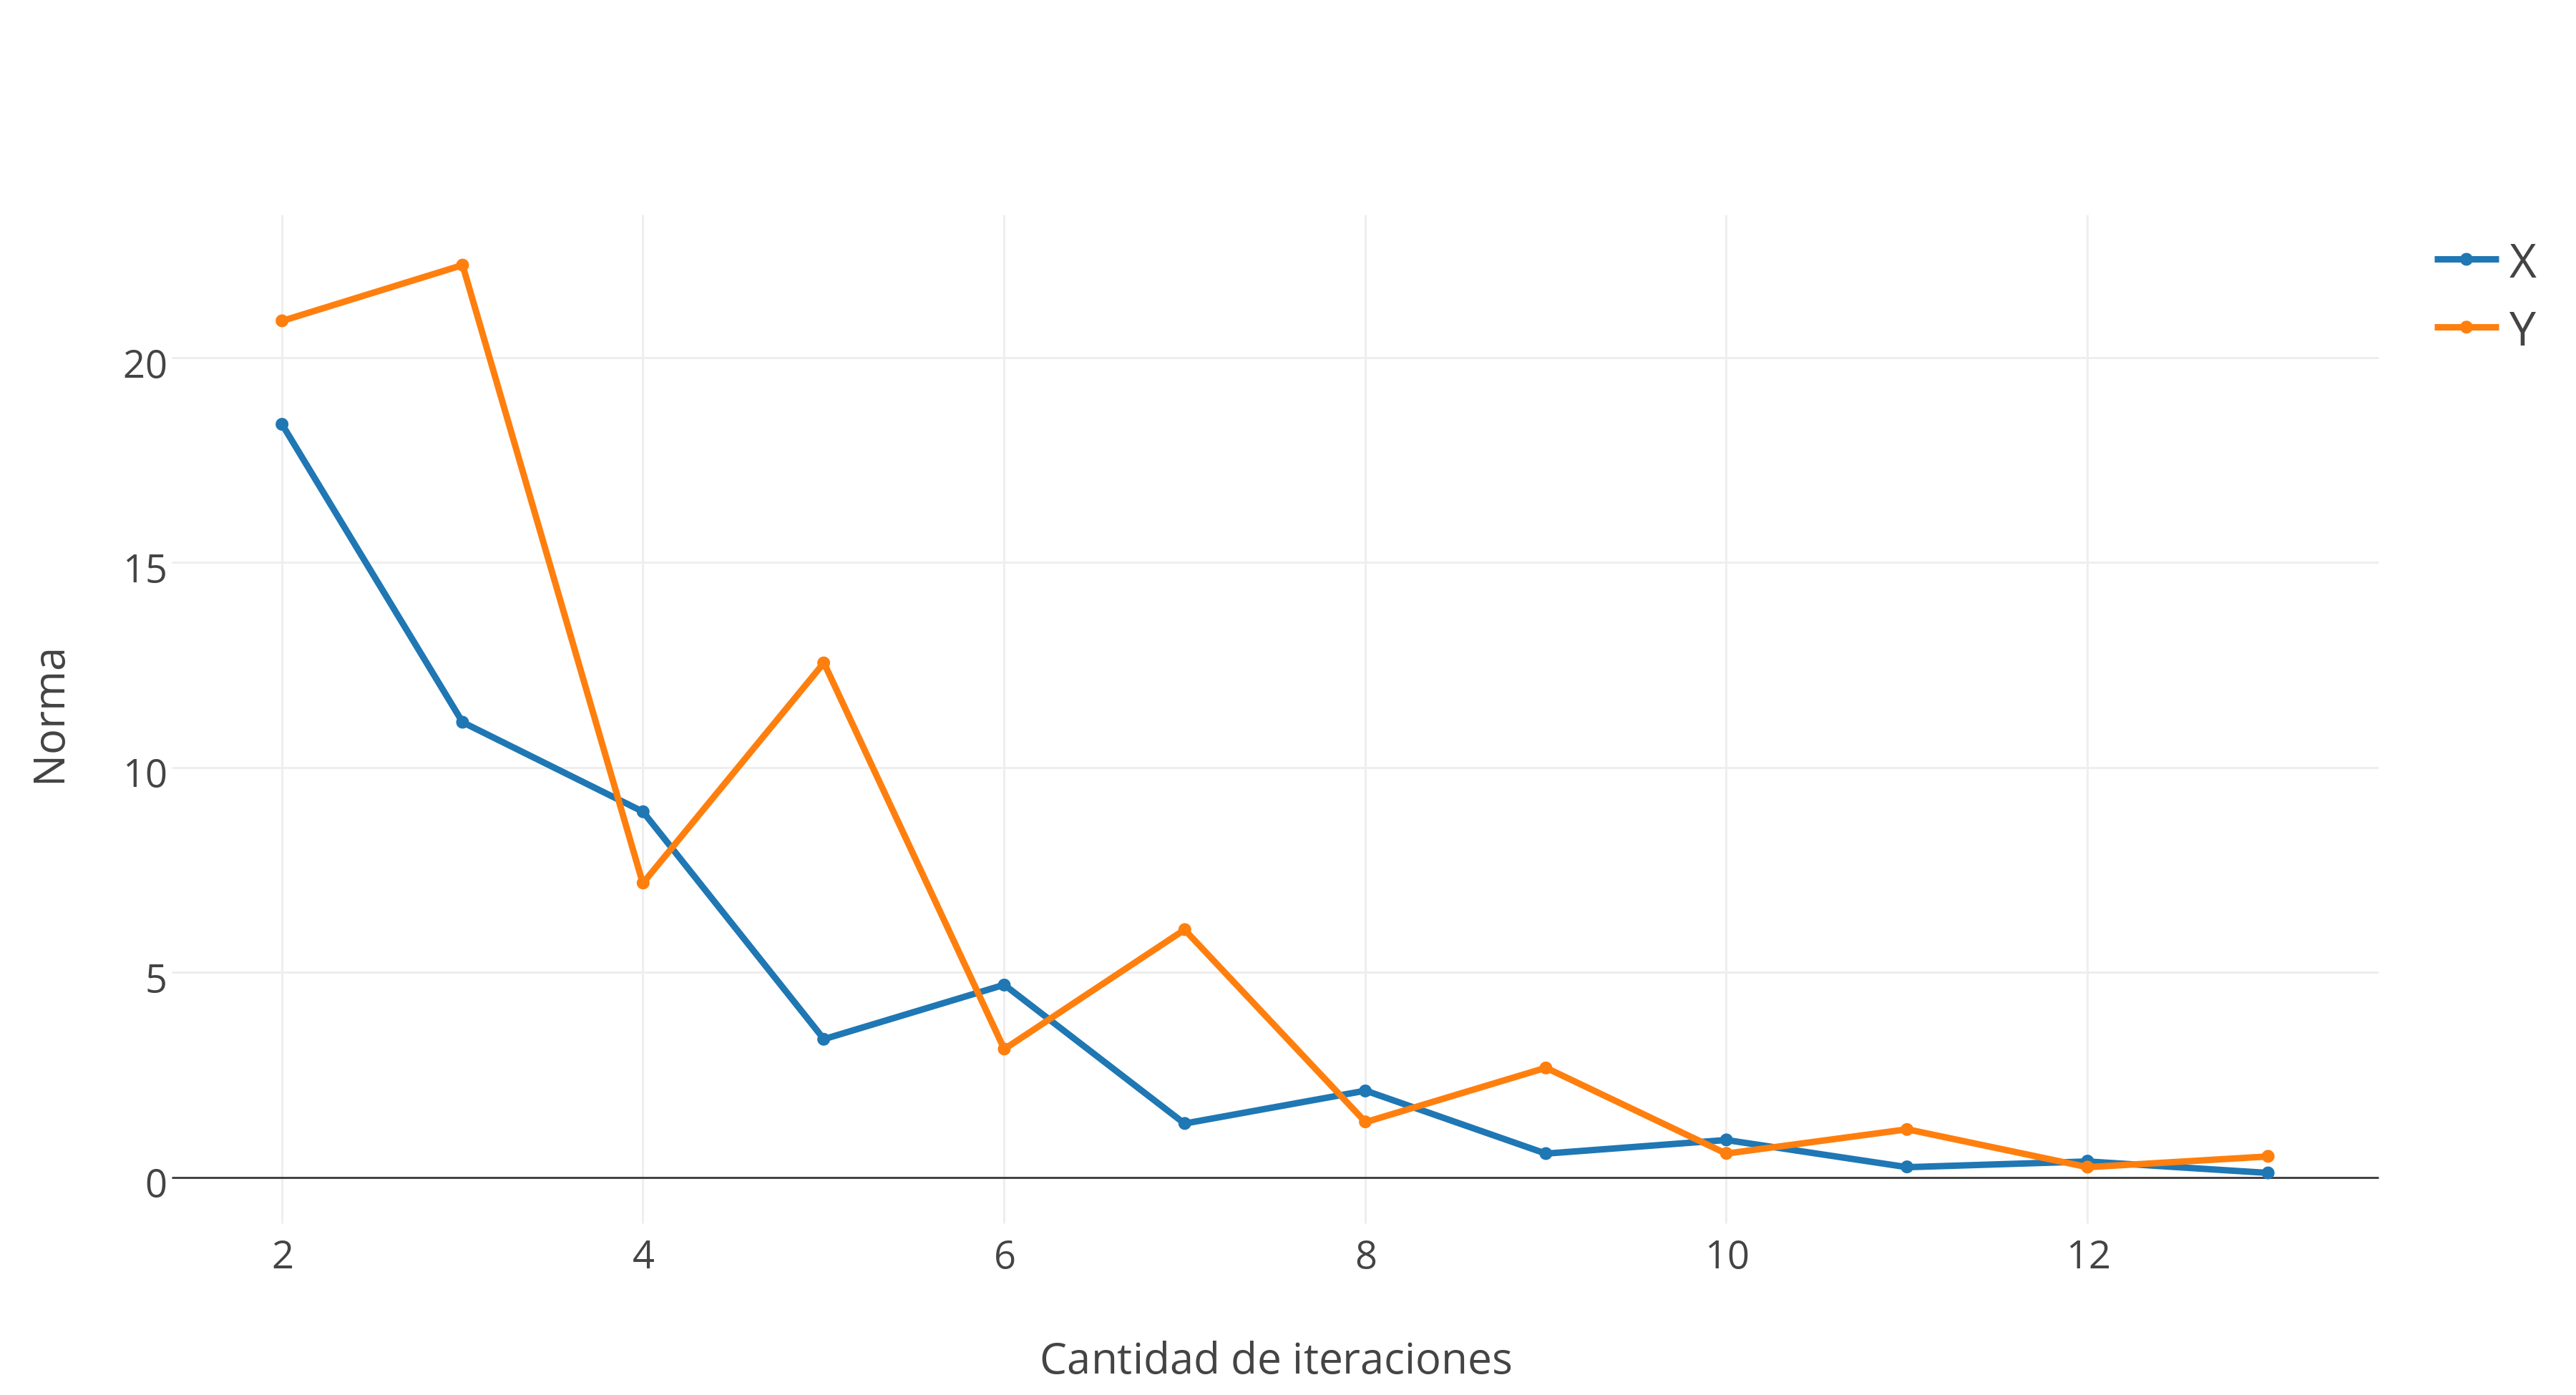
\includegraphics[scale=0.50]{imagenes/exp12/moviesHITS.png}
	\caption{Variaci\'on de la norma de X e Y en cada iteraci\'on para la Red Movies}
	\label{nombreparareferenciar}
	\textit{La cantidad de iteraciones llevadas a cabo por el algoritmo fue de 29.}
  \end{center}
\end{figure}
\newpage
\begin{figure}[h!]
  \begin{center}
	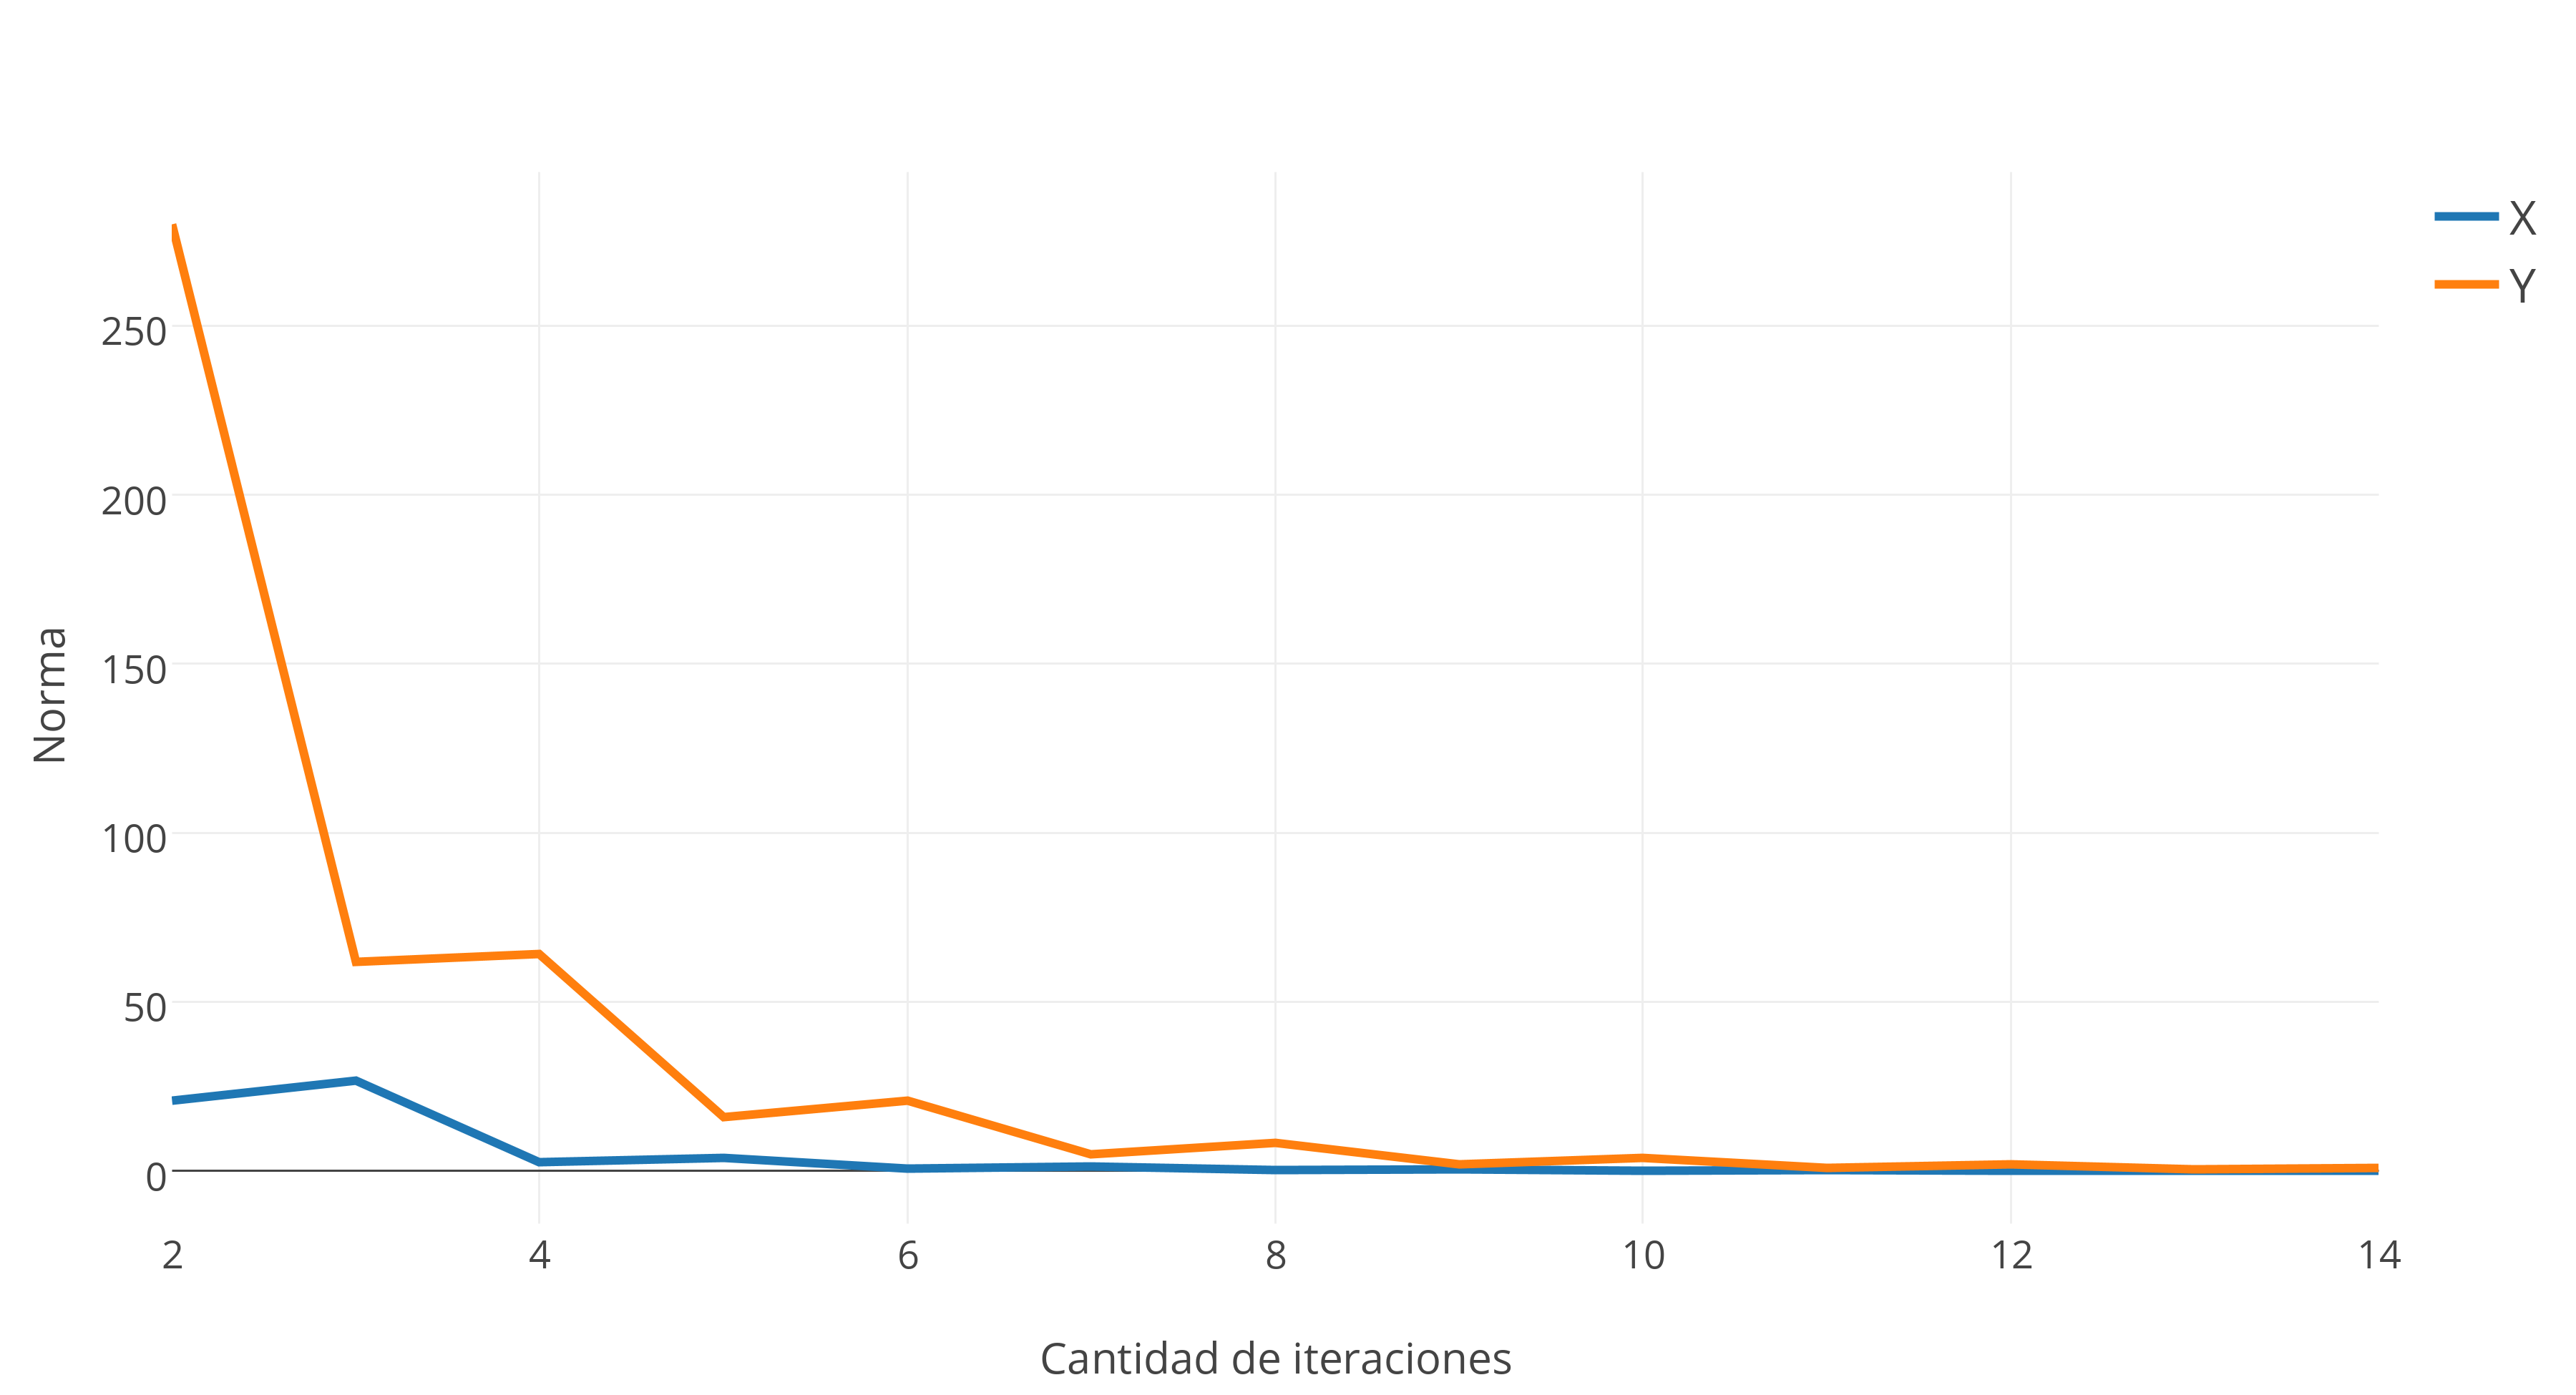
\includegraphics[scale=0.50]{imagenes/exp12/stanfordHITS.png}
	\caption{Variaci\'on de la norma de X e Y en cada iteraci\'on para la Red Stanford}
	\label{nombreparareferenciar}
	\textit{La cantidad de iteraciones llevadas a cabo por el algoritmo fue de 28.}
  \end{center}
\end{figure}

\begin{figure}[h!]
  \begin{center}
	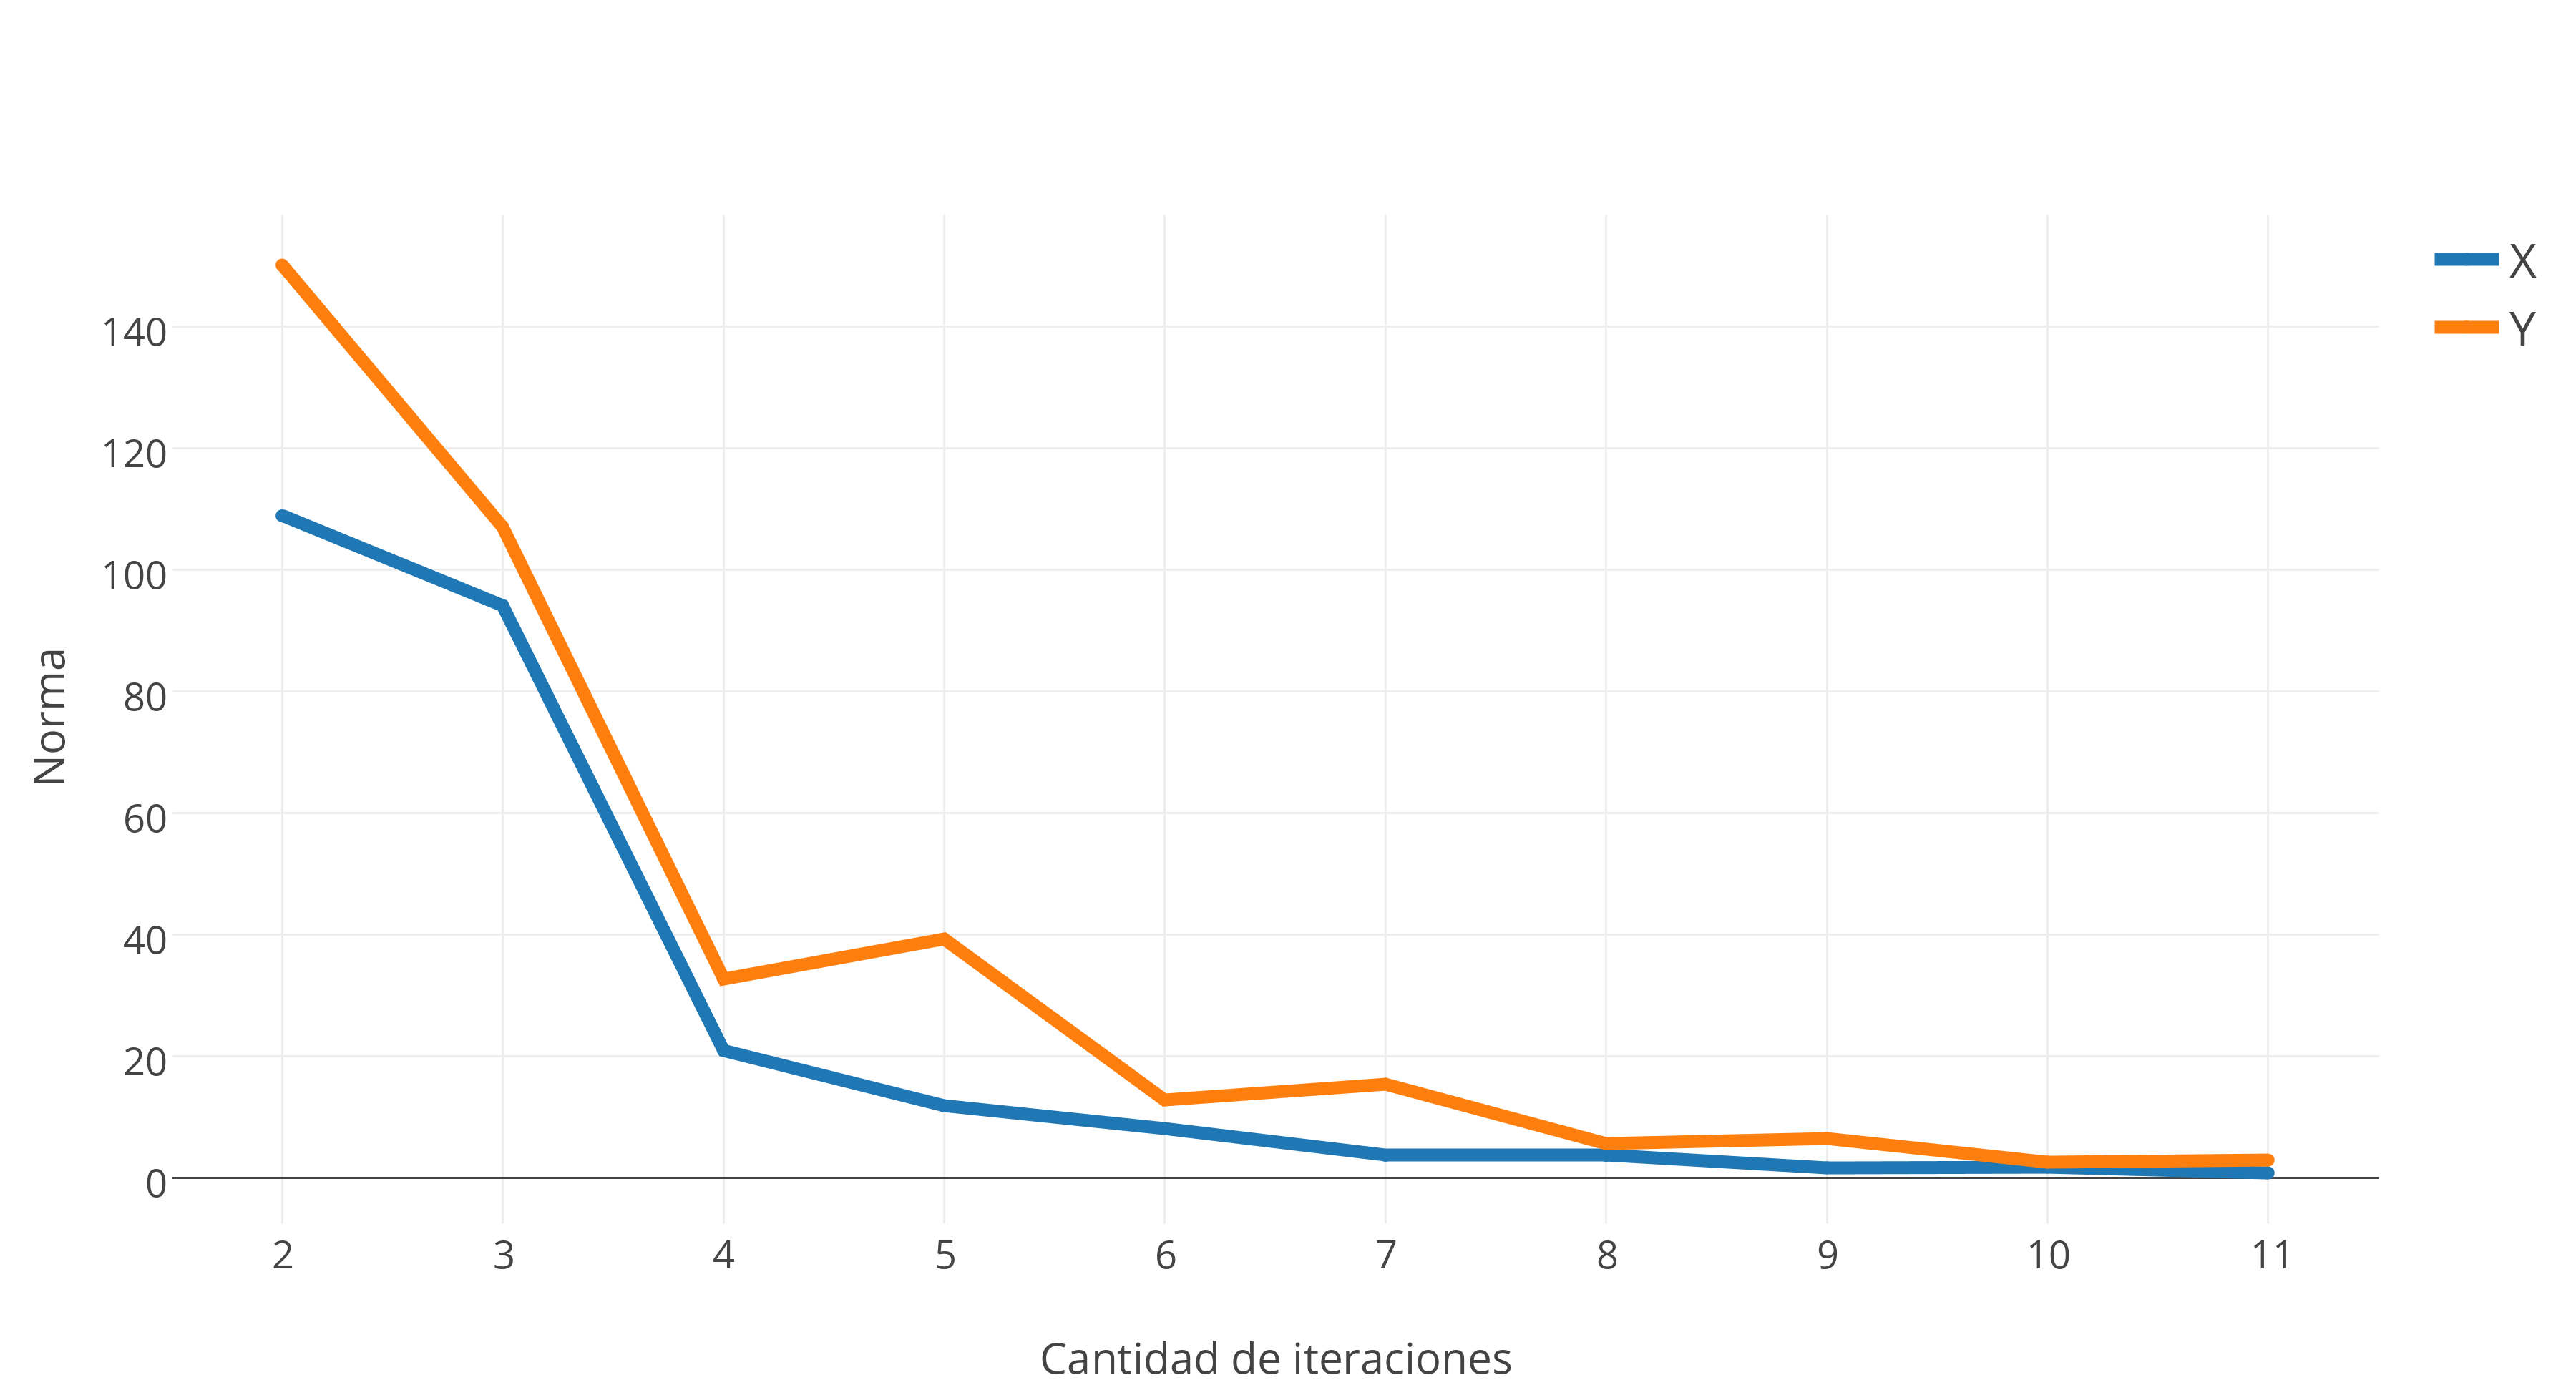
\includegraphics[scale=0.50]{imagenes/exp12/notredameHITS.png}
	\caption{Variaci\'on de la norma de X e Y en cada iteraci\'on para la Red Notre Dame}
	\label{nombreparareferenciar}
	\textit{La cantidad de iteraciones llevadas a cabo por el algoritmo fue de 31.}
  \end{center}
\end{figure}
\indent En todos los gr\'aficos presentados se puede apreciar que la norma de los vectores X e Y converge a cero. Cabe destacar un suceso llamativo: en las primeras iteraciones los valores de la norma de la diferencia de X con los de Y son alternadamente muy cercanos y muy lejanos. No se puede unificar esta observaci\'on para todos los casos, ya que cada uno presenta sus propias anomal\'ias. \\
\indent En el caso de red m\'as chica (\emph{Complexity}), si bien se puede apreciar esta alternancia entre la distancia del valor de X e Y, el vector X se ubica por encima del Y en las primeras iteraciones para luego situarse muy cercanos hasta converger a cero. En el caso de la segunda red (\emph{Abortion}), se puede apreciar un comportamiento parecido donde el vector X se sit\'ua por encima del Y, sin embargo alternadamente van adquiriendo un valor muy similar que hace que el valor de Y sea mayor al de X. La \'ultima red de tama\~no mediano (\emph{Movies}) reitera el comportamiento de las dos anteriores, s\'olo que en las iteraciones que los vectores X e Y antes estaban muy cerca ahora se cruzan ubic\'andose siempre el vector Y por encima del X en mayor proporci\'on que antes. \\

\indent En el caso de las redes grandes (\emph{Notre Dame y Stanford}), sus comportamientos son muy similares entre s\'i. El vector Y se sit\'ua en todo momento por encima del X, y luego de una mayor cantidad de iteraciones se observa que ambos vectores convergen a cero.\\
\\
\indent Algo notorio que se observa es que: cuanto m\'as grande sea la red, una mayor cantidad de iteraciones es necesaria para llegar al valor que converge.\\
\newpage
\subsection{Factor Temporal}
\textcolor{red}{PONER ACA LOS EXPERIMENTOS SOBRE EL VECTOR INICIAL Y LA CANTIDAD DE ITERACIONES
Y para el algoritmo de PageRank, ver como dan los resultados para cada c, para la misma red y ver qué valor de c podría tener sentido. fruta++ }
\\
\indent El factor tiempo en el uso es una caracter\'istica importante de los algoritmos si se van a computar online, ya que es tiempo que el usuario debe esperar hasta obtener su resultado. Si bien el algoritmo de PageRank es computado, generalmente, online; el de HITS no lo es ya que debe primero armar la red con la que va a trabajar.\\
\\
\indent A continuaci\'on se incluyen los gr\'aficos de las mediciones de tiempo de ejecuci\'on de los m\'etodos, para ello no se incluye el costo de armado de la matriz con los datos pasados en el archivo de entrada como par\'ametro.\\
El siguiente gr\'afico mide el tiempo de c\'omputo para redes de tama\~no mediano.

\begin{figure}[h!]
  \begin{center}
	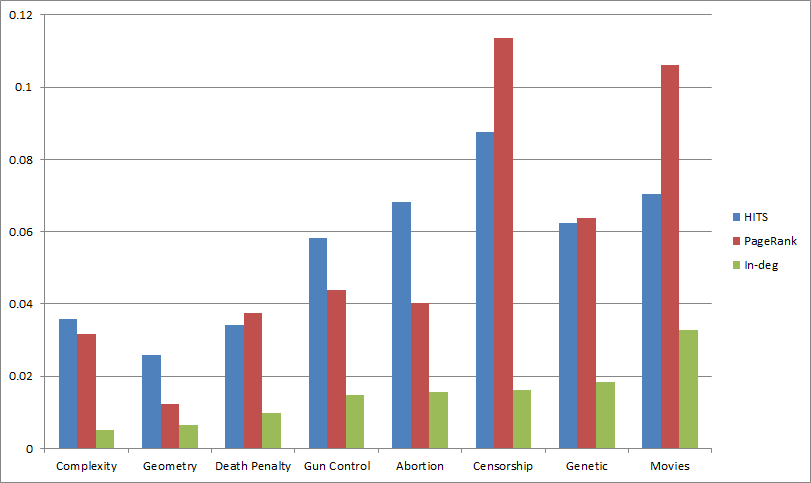
\includegraphics[scale=0.50]{imagenes/expTiempo/tiemposMedianos.png}
	\caption{Medici\'on de los tres m\'etodos para redes medianas}
	\label{nombreparareferenciar}
  \end{center}
\end{figure}

El siguiente gr\'afico mide el tiempo de c\'omputo para redes de tama\~no grande.\\
\begin{figure}[h!]
  \begin{center}
	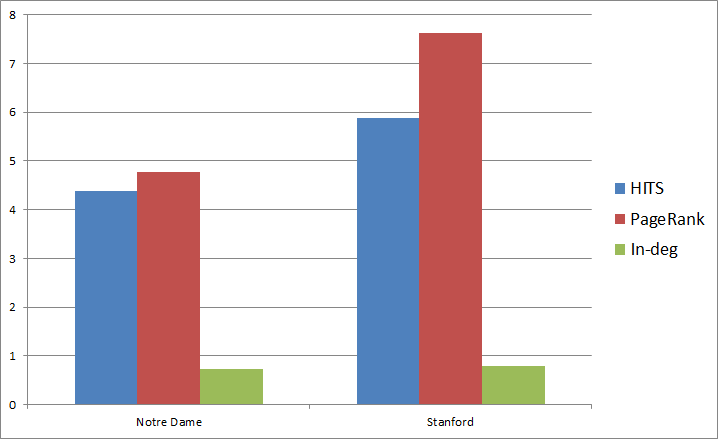
\includegraphics[scale=0.50]{imagenes/expTiempo/tiemposGrandes.png}
	\caption{Medici\'on de los tres m\'etodos para redes grandes}
	\label{nombreparareferenciar}
  \end{center}
\end{figure}

\textcolor{red}{Gus la tiene re clara aca, yo no tengo ni idea. perdon \\
NOS QUEDO PENDIENTE? o es lo de gus?(lo que sigue aca abajo) ...} \\
Un trabajo que nos qued\'o pendiente es experimentar cu\'ales son los factores que influyen en el aumento del tiempo para el algor\'itmo de HITS entre la dimensi\'on de la matriz, la cantidad de elementos o mismo la composici\'on del grafo de la red. \\
\newpage

\subsection{Ejemplos ilustrativos y comparaci\'on de los tres M\'etodos}


Con el fin de poner a prueba experimentalmente el conocimiento aprendido de manera teórica acerca de los algoritmos, destinamos esta sección a la presentación de las hipótesis que formulamos acerca de sus funcionamientos, a los ensayos dirigidos a partir de las mismas y a los resultados obtenidos a partir de aquellos junto con una serie de posibles explicaciones a los comportamientos observados.

\textbf{Hipótesis 1: \itshape{Si se toma un conjunto de páginas base (es decir, no apuntadas por ninguna otra de la red) que tengan links salientes hacia un conjunto de webs de menor dimensión cuyas direcciones se encuentran muy apuntadas, entonces mientras que el algoritmo de HITS va a considerar importantes dichas páginas, no encabezarán el listado de webs sugerido por un algoritmo de PageRank}}\\


Para contrastar esta hipótesis diseñamos una red que cuya particularidad es que existen conjuntos de webs poco apuntadas que poseen links salientes a un grupo reducido de páginas que - en lo posible - no apunten recíprocamente a aquellas. La idea es generar una instancia en la cual existan un conjunto de autoridades destacables  que concedan a las páginas que las apuntan una fuerte identidad de hubs, para poder anailzar cómo jerarquiza a estas últimas cada método.

Los resultados obtenidos para la Red 1  (citada continuación) son los presentados en las figuras \ref{hitsa1}, \ref{hitsh1} y 15.

\textbf{Red 1:}\\

\begin{tabular}{l l}
1 & Empirismo \\
2 & Racionalismo \\
3 & Humanismo \\
4 & Crítica de la razón pura \\
5 & Metafísica \\
6 & Discurso del método \\
7 & Lógica de Port-Royal \\
8 & Principio de razon suficiente \\
9 & Juicio sintáctico a priori \\
10 & Investigación sobre el entendimiento humano \\
11 & Razonamiento inductivo \\
12 & Instrumentalismo \\
13 & Ecdótica \\
14 & Robert G. Ingersoll \\
15 & Antihumanismo \\
\end{tabular}

\newpage
\begin{figure}[h!]
  \begin{center}
	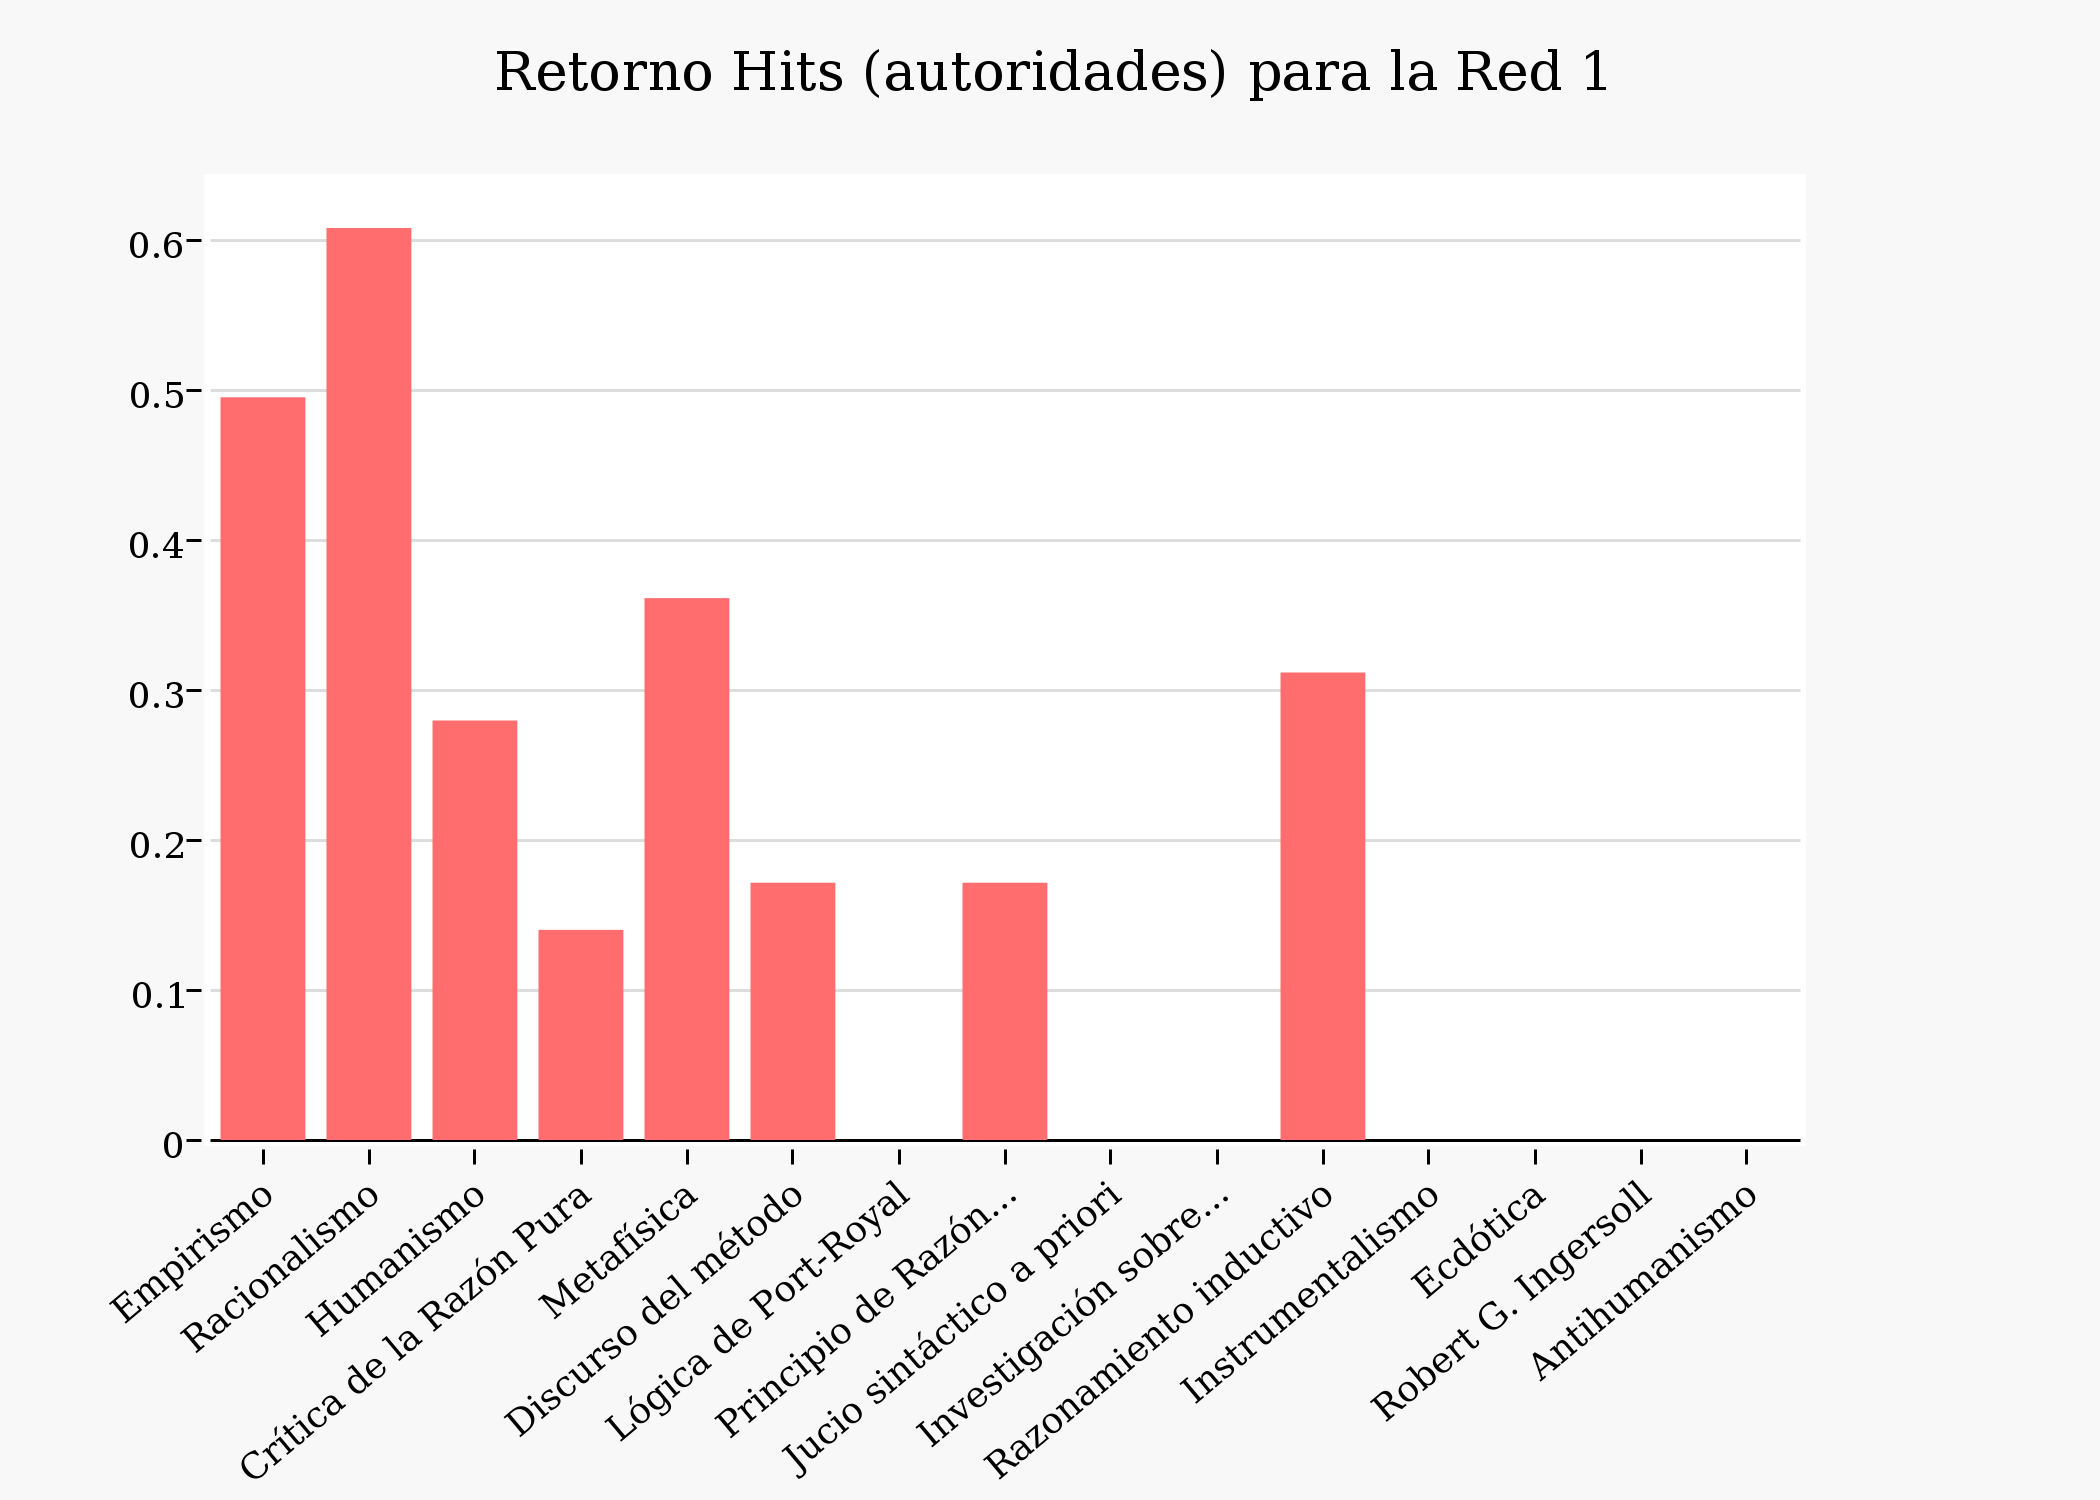
\includegraphics[scale=0.66]{imagenes/Exp1/hitsA1}
	\caption{}	
	\label{hitsa1}
  \end{center}
\end{figure}

\begin{figure}[h!]
  \begin{center}
	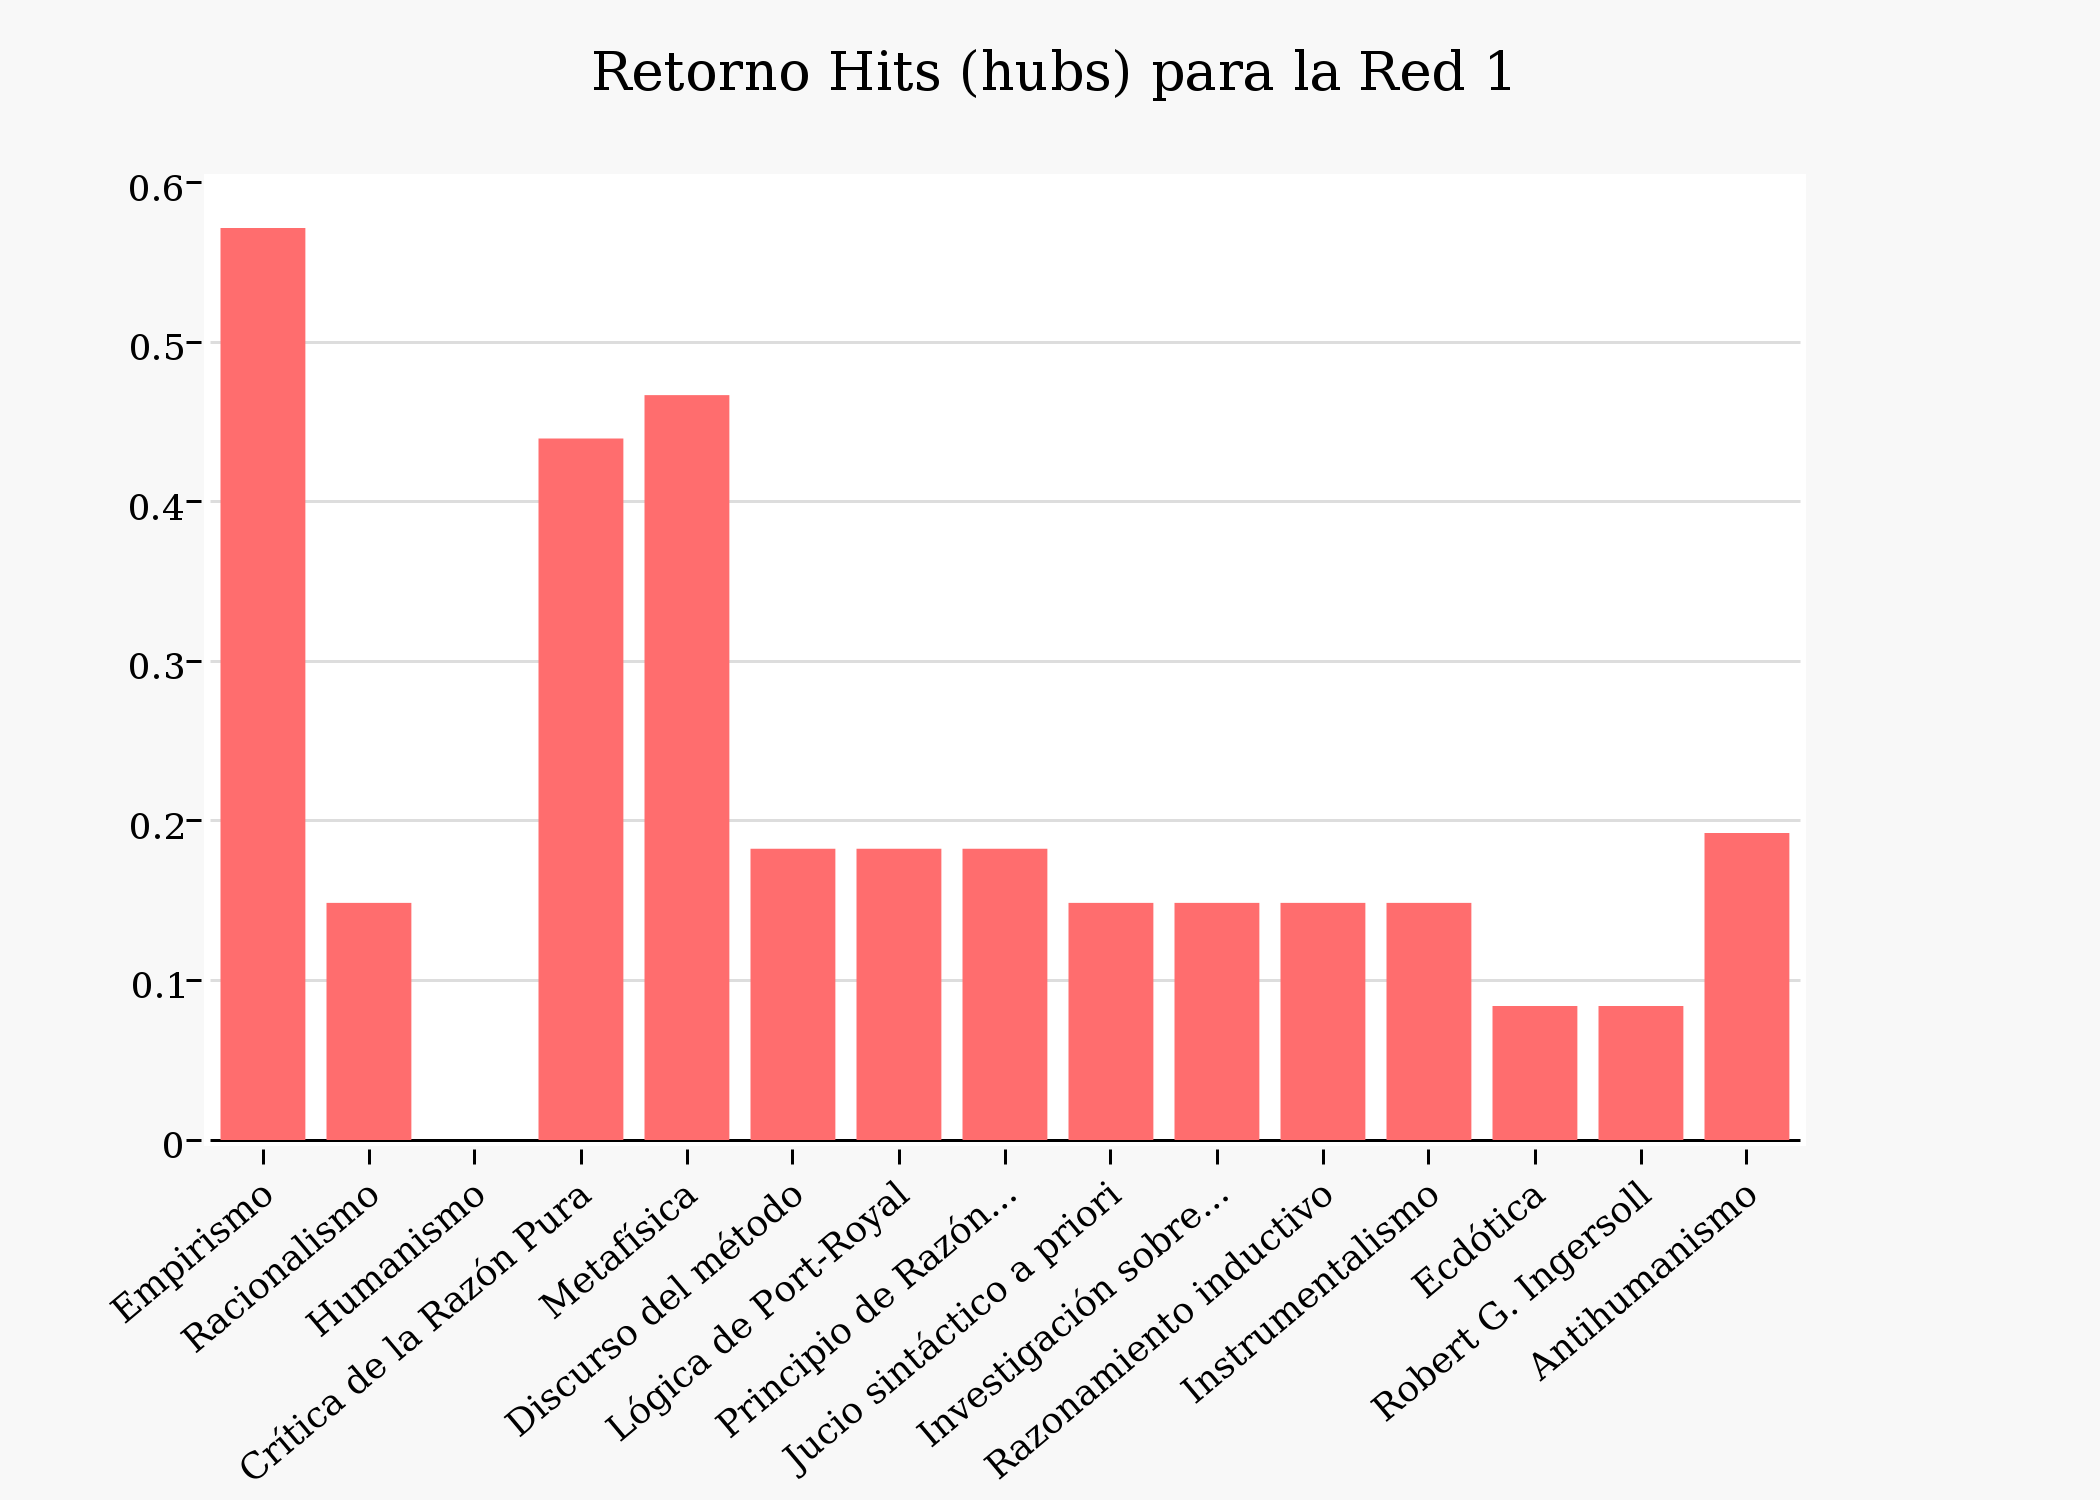
\includegraphics[scale=0.66]{imagenes/Exp1/hitsH1}
	\caption{}
	\label{hitsh1}
  \end{center}
\end{figure}

\newpage

\begin{figure}[h!]
  \begin{center}
	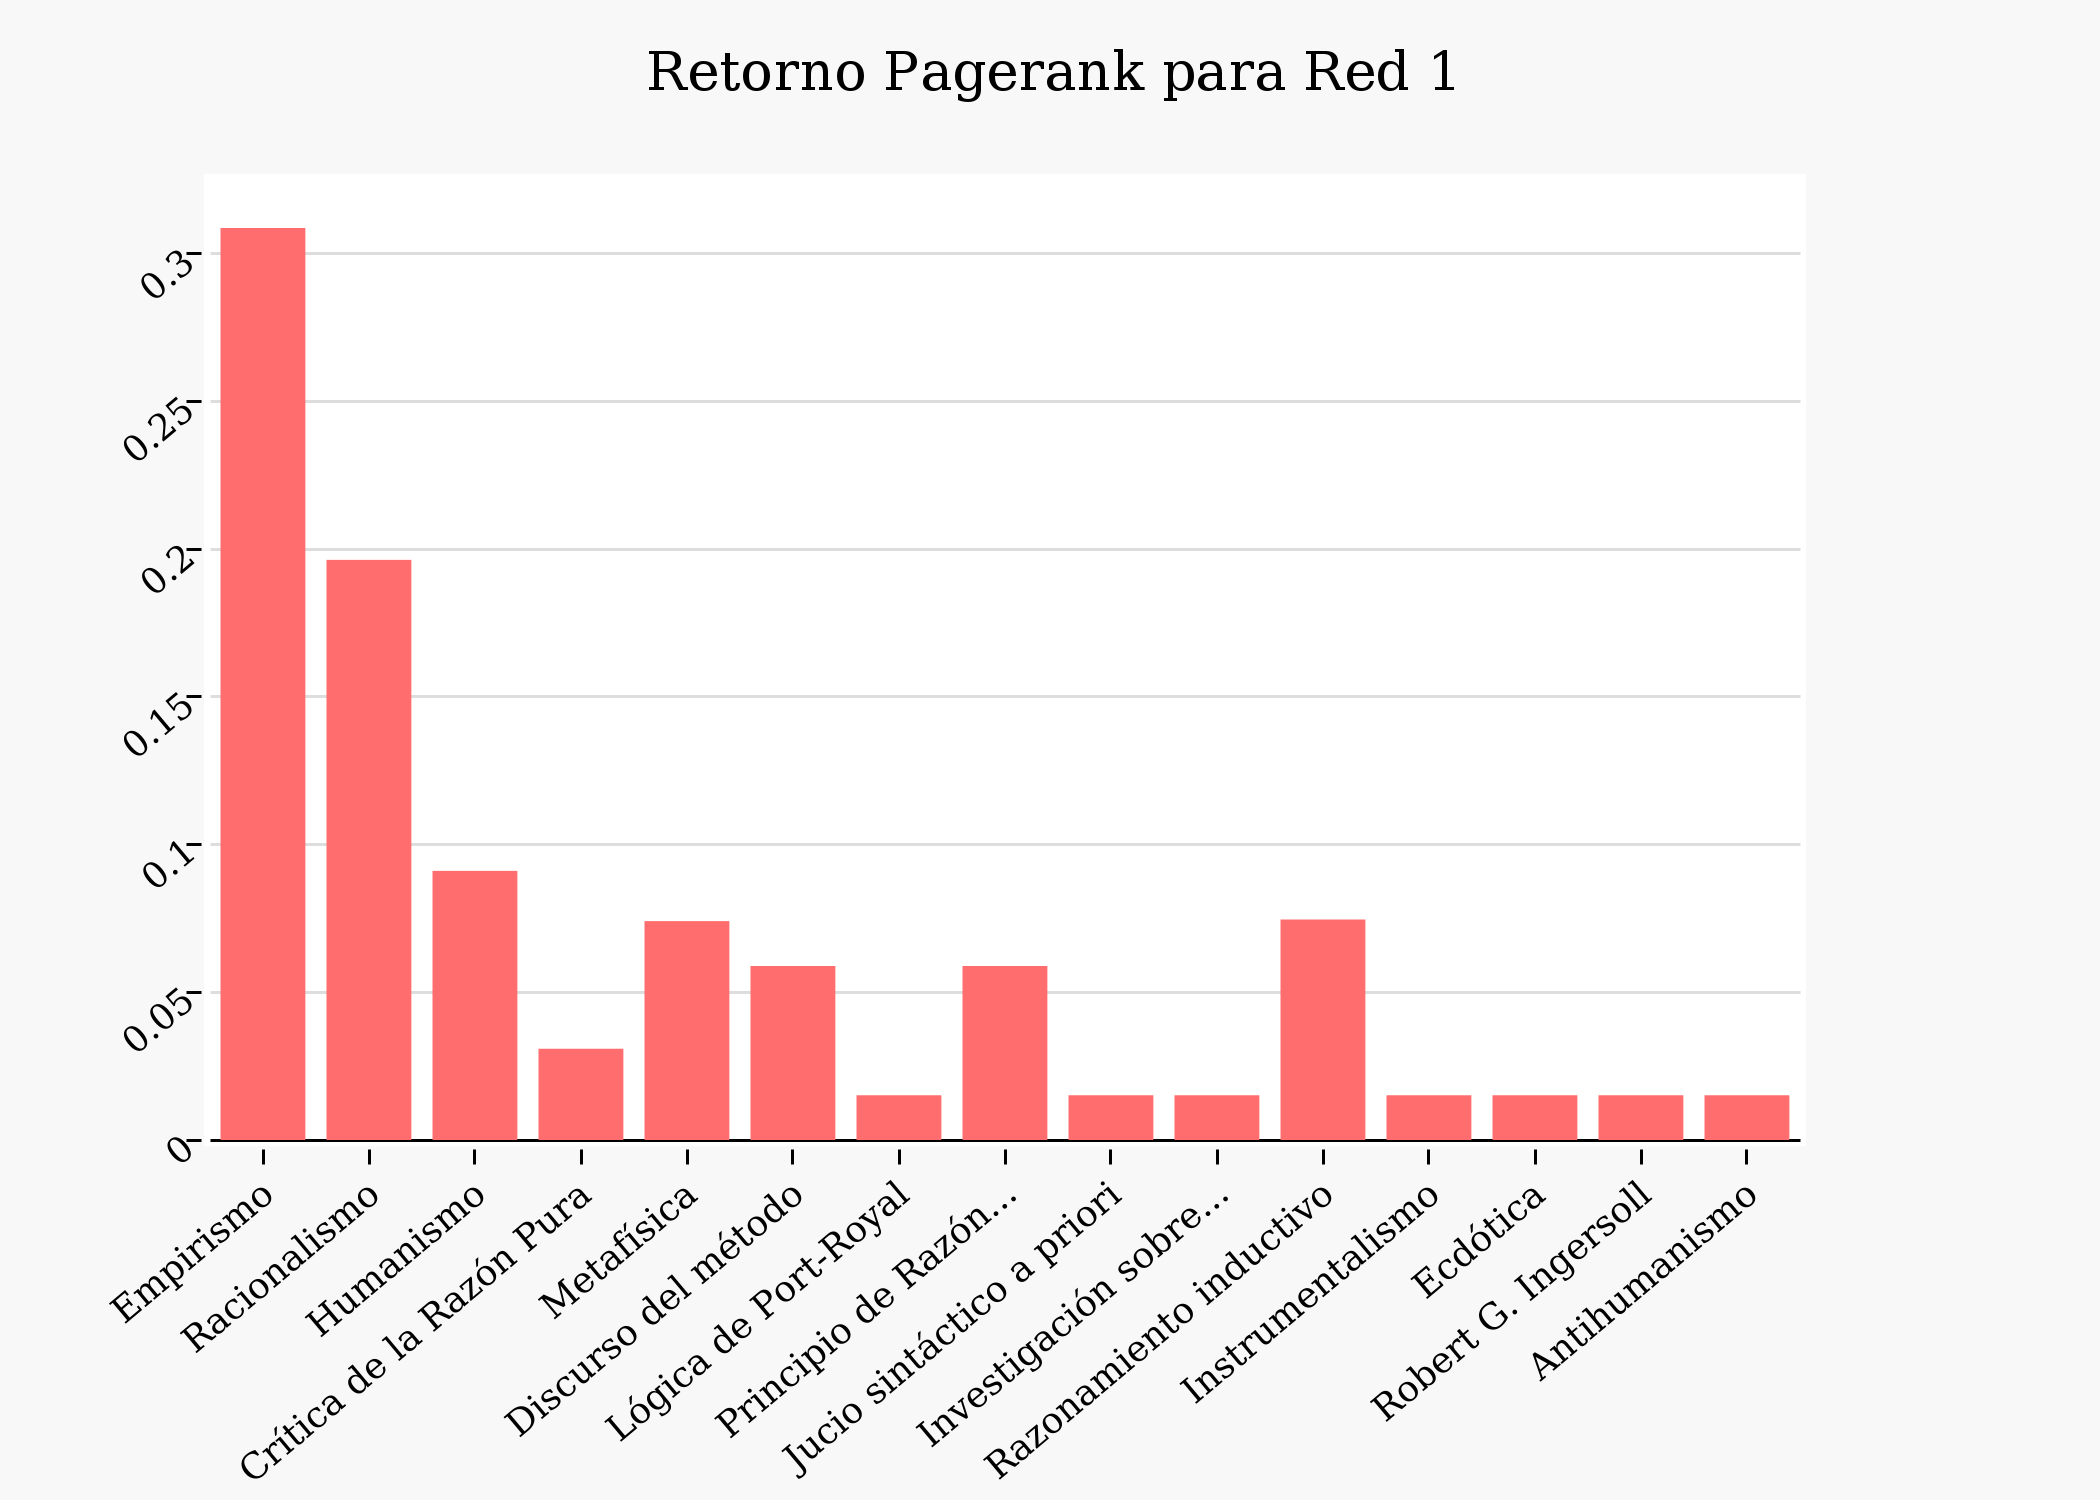
\includegraphics[scale=0.66]{imagenes/Exp1/PR1}
	\caption{}
	\label{PR1}
  \end{center}
\end{figure}



En los gráficos adjuntados se puede observar que las webs mejor puntuadas para PageRank resultaron\\ ser \\
Empirismo \\
Racionalismo \\
Humanismo \\
Metafísica \\
Razonamiento inductivo \\
Principio de la razón \\
\indent Si analizamos los resultados de Hits para organizar las autoridades, encontramos en este caso más páginas coincidentes con las priorizadas con el algoritmo de Pagerank. De hecho, las cinco páginas a las que éste último método concede las primeras posiciones, son las mismas que pueden encontrarse en los cinco principales puestos resultantes de Hits para autoridades.  \\
\indent Ahora bien, Si comparamos con la jerarquía sugerida por Hits (hubs), notamos que una de las webs anteriormente mencionadas (humanismo) tiene valor nulo, mientras que muchas otras sugeridas por este método ni siquiera figuran entre las que PageRank considera webs de importancia (crítica a la razón pura, antihumanismo, etc.). \\
\indent Los acuerdos entre ambos gráficos se dan en los casos de las páginas ``Empirismo'' y ``Metafísica'', las cuales poseen más links salientes que todas las demás (y apuntan a la mejor autoridad, que es racionalismo) y, a su vez, son apuntadas por más de dos webs. En otras palabras, estas dos páginas no nos interesan realmente a los fines analíticos de la hipótesis en cuestión, dado que al poder ser considerados ``hibridos'' entre hubs y autoridades, no nos permiten emitir conclusiones claras al respecto.\\
\indent Dicho esto, si dercartaramos estos dos casos notaríamos que las coincidencias entre los resultados arrojados son muy disímiles.\\
\indent Esto nos hace pensar que el nivel de relación que puedan tener los resultados de PageRank con los de HITS, dependerá diréctamente del criterio que se tome para ordenar jerárquicamente los resultados de HITS. Con este ejemplo podemos deducir que si los hubs fueran considerados más importantes que las autoridades, entonces las coincidencias entre los principales resultados de los métodos enunciados serán menores que en el caso en que el nivel de prioridades entre hubs y autoridades se intercambie.


\newpage

\textbf{Hipótesis 2: \itshape{Si se toma la misma red y se le incluye una web que apunte a las mayores autoridades, entonces ésta pasará a ser el hub más importante de la nueva red. }}\\

Para intentar contrastar esta proposición tomamos la Red 1 presentada en la \textit{hip\'otesis} $1$, le agregamos una web nueva (\textit{``Escuelas Filosóficas''}), ejecutamos los algoritmos de PageRank y de HITS y luego analizamos los datos obtenidos en este apartado en conjunto con los arrojados en el inmediato anterior.\\

Los resultados son los presentados en las figuras \ref{hitsa2}, \ref{hitsh2} y \ref{pr2}, mientras que en la figura \ref{grafo2} se puede observar el grafo de la nueva web.

\textbf{Red 2:}\\

\begin{tabular}{l l}
1 & Escuela Filosófica \\
2 & Empirismo \\
3 & Racionalismo \\
4 & Humanismo \\
5 & Crítica de la razón pura \\
6 & Metafísica \\
7 & Discurso del método \\
8 & Lógica de Port-Royal \\
9 & Principio de razon suficiente \\
10 & Juicio sintáctico a priori \\
11 & Investigación sobre el entendimiento humano \\
12 & Razonamiento inductivo \\
13 & Instrumentalismo \\
14 & Ecdótica \\
15 & Robert G. Ingersoll \\
16 & Antihumanismo \\
\end{tabular}

\begin{figure}[h!]
  \begin{center}
	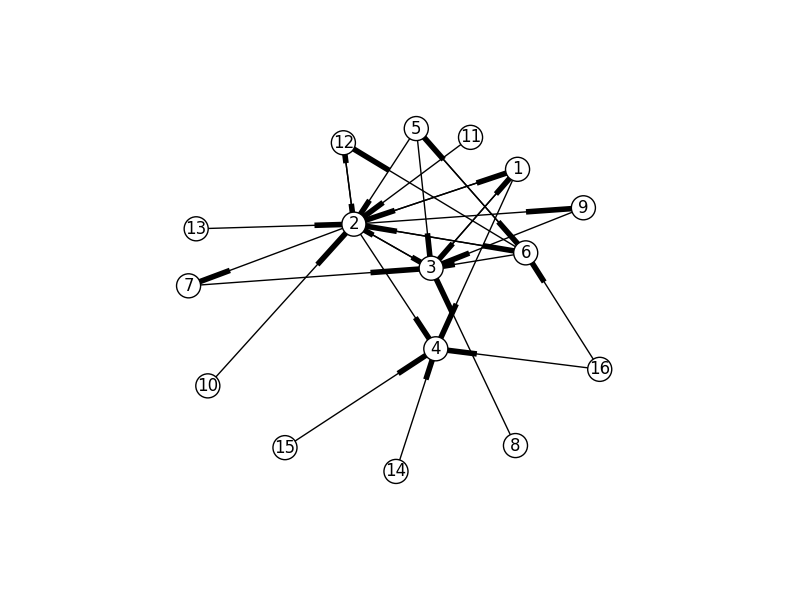
\includegraphics[scale=0.6]{imagenes/Exp2/grafo2}
	\caption{}
	\label{grafo2}
  \end{center}
\end{figure}
\newpage
\begin{figure}[h!]
 \begin{center}
	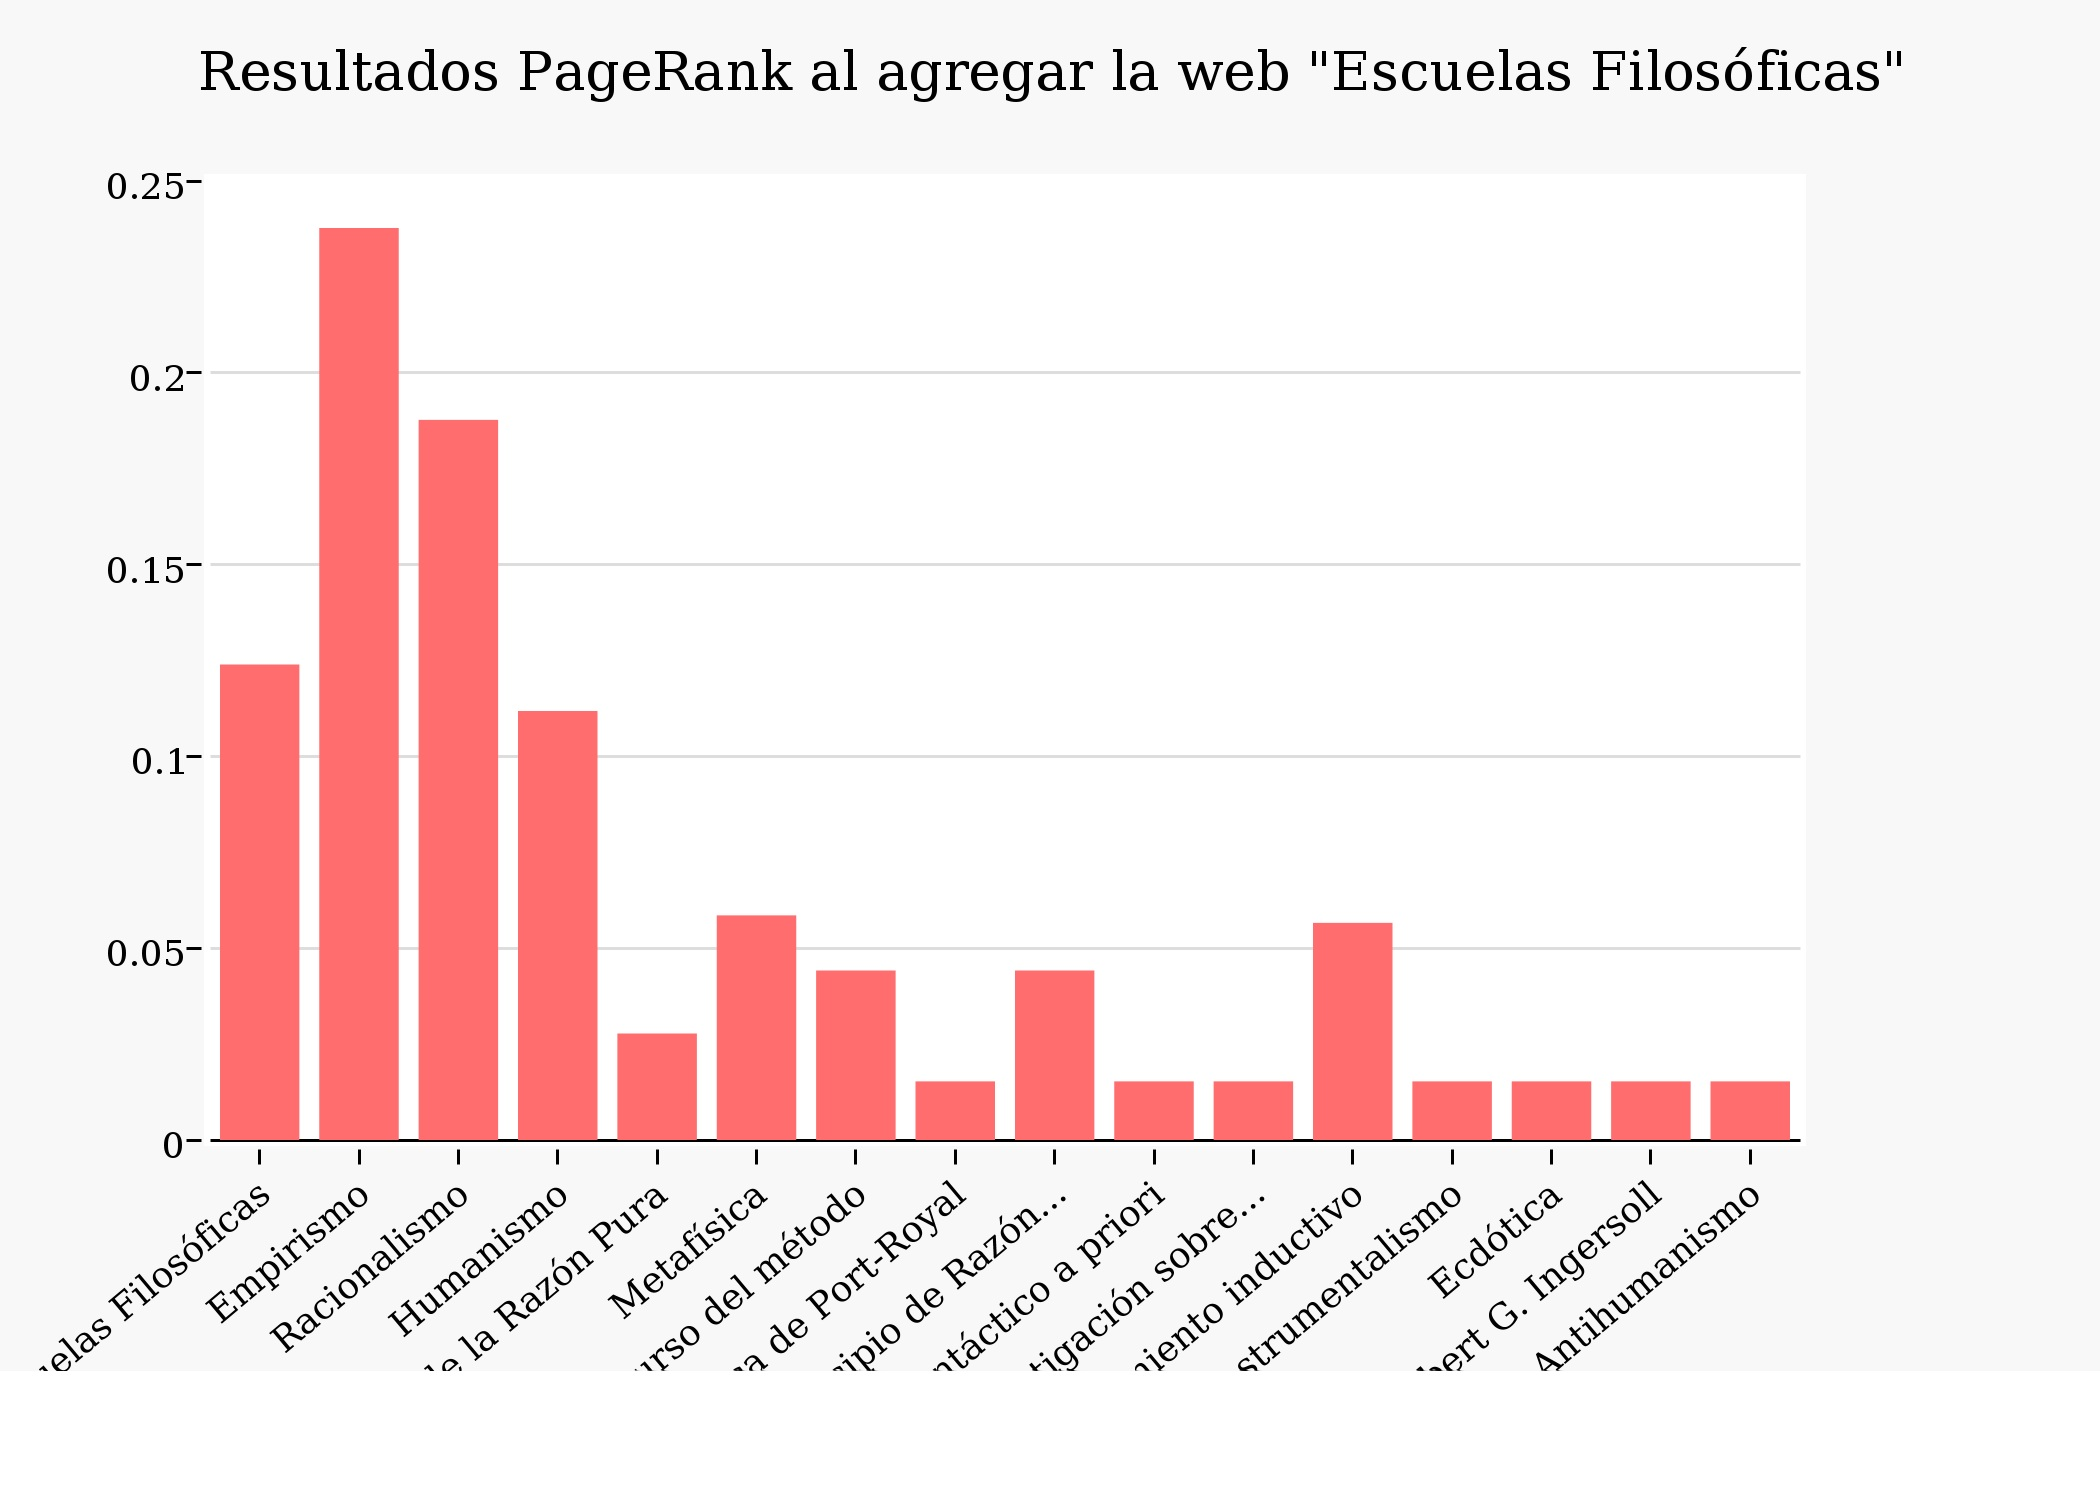
\includegraphics[scale=0.3]{imagenes/Exp2/PR2}
	\caption{}
	\label{hitsa2}
  \end{center}
\end{figure}
\newpage
\begin{figure}[h!]
  \begin{center}
	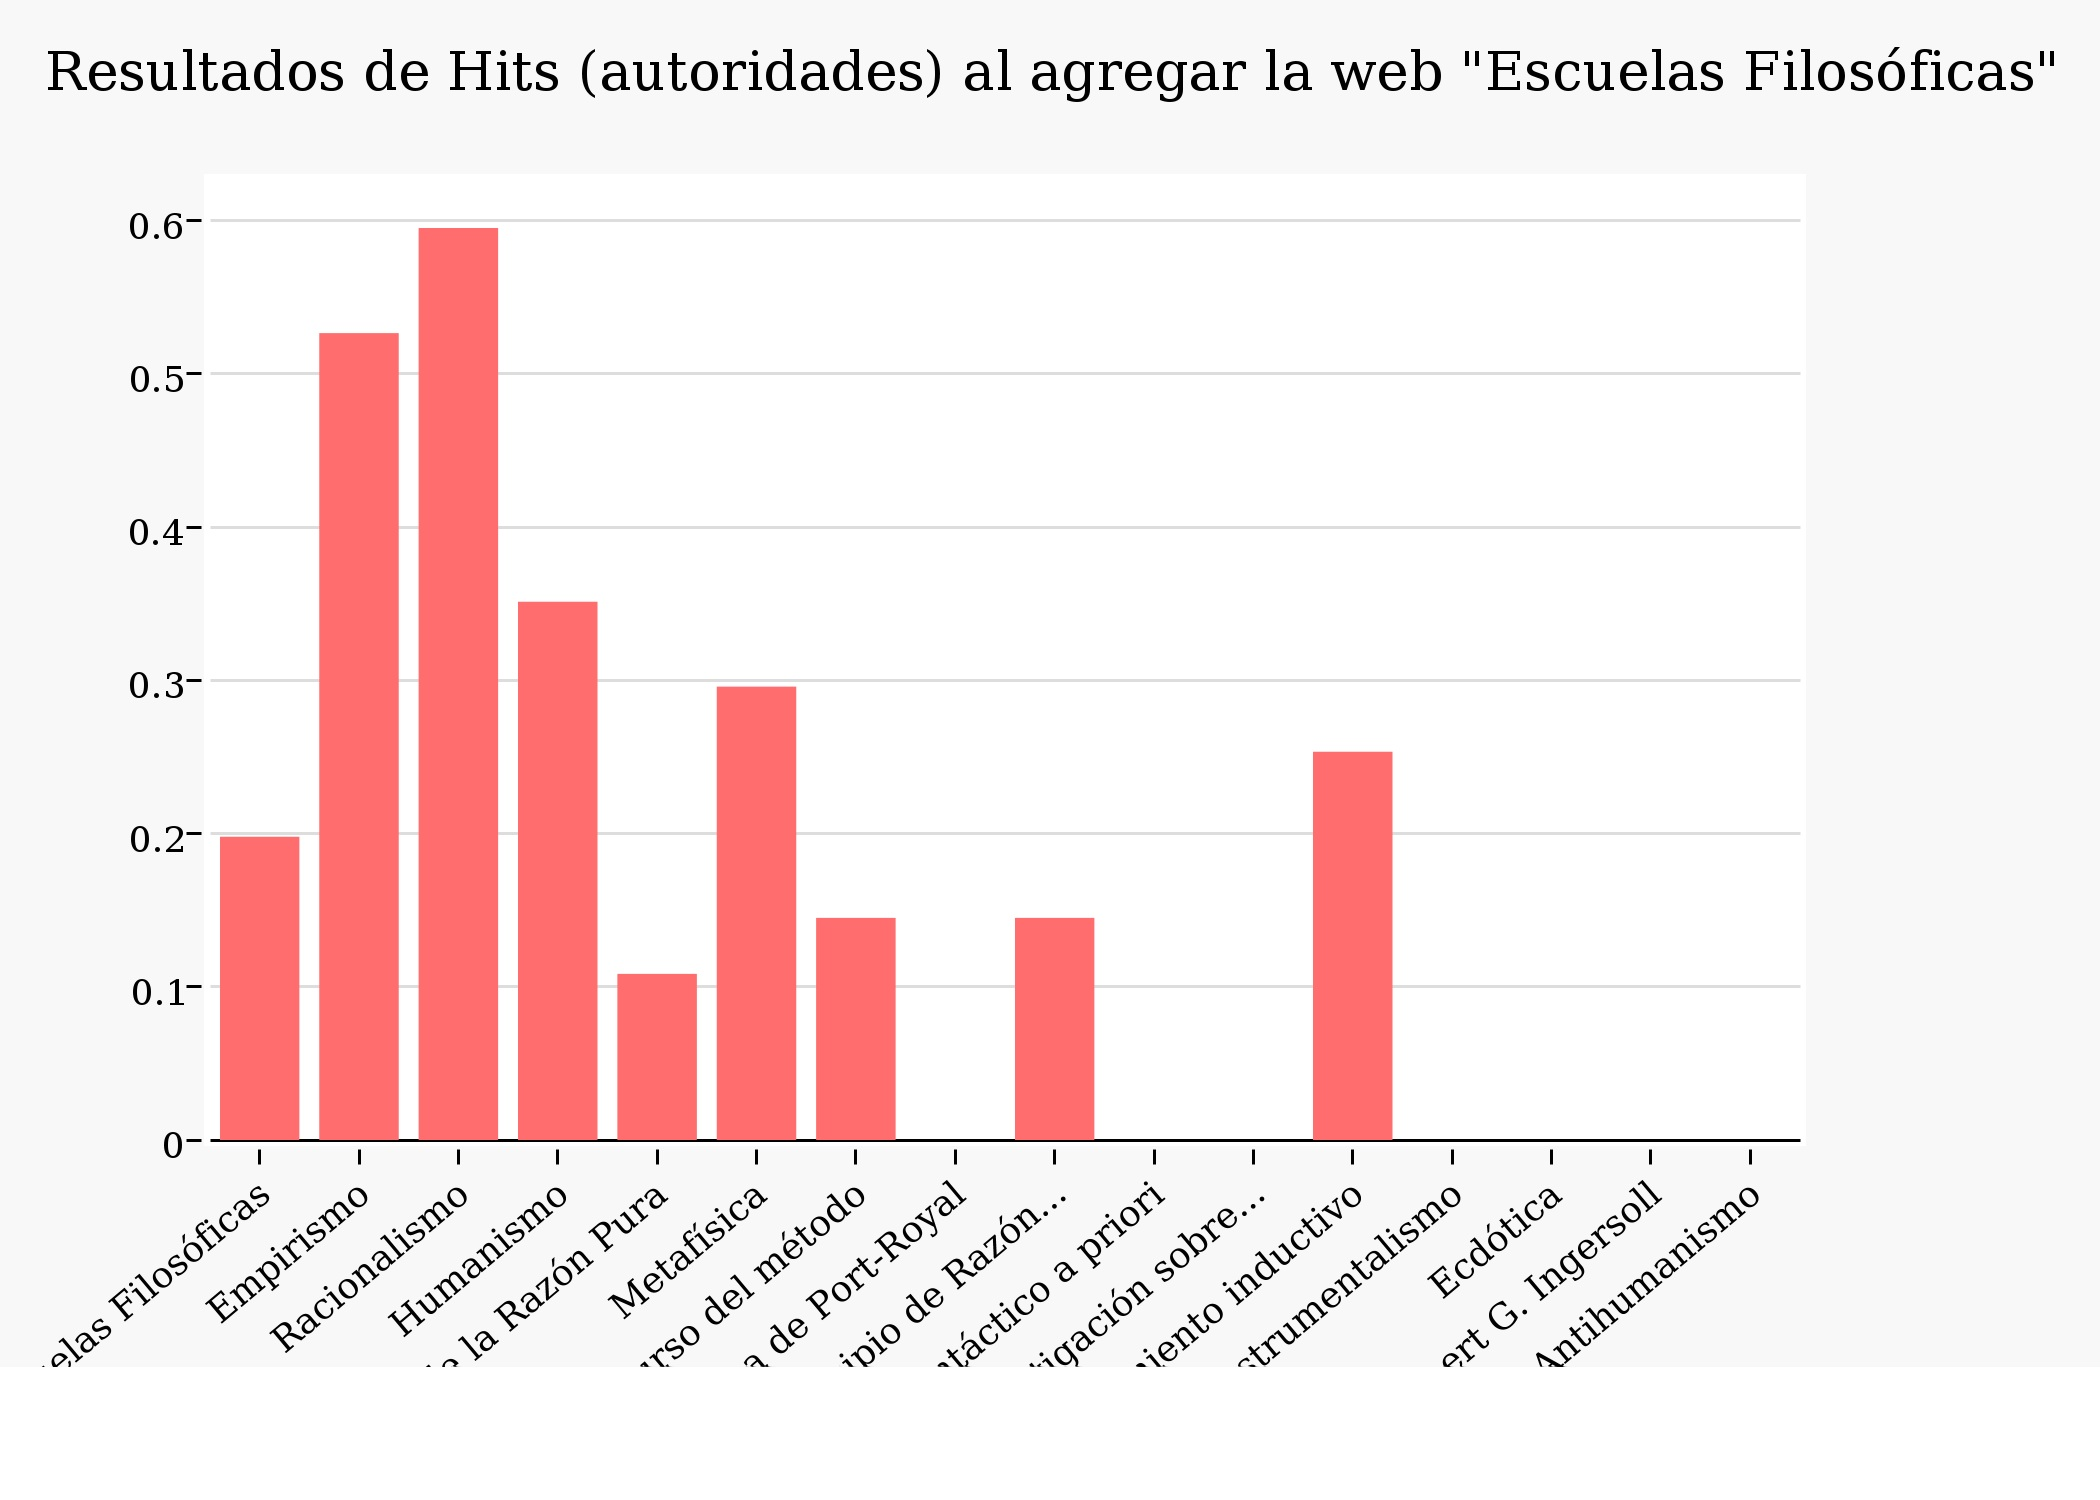
\includegraphics[scale=0.3]{imagenes/Exp2/hitsa2nuevo}
	\caption{}
	\label{pr2}
  \end{center}
\end{figure}
\newpage
\begin{figure}
 \begin{center}
	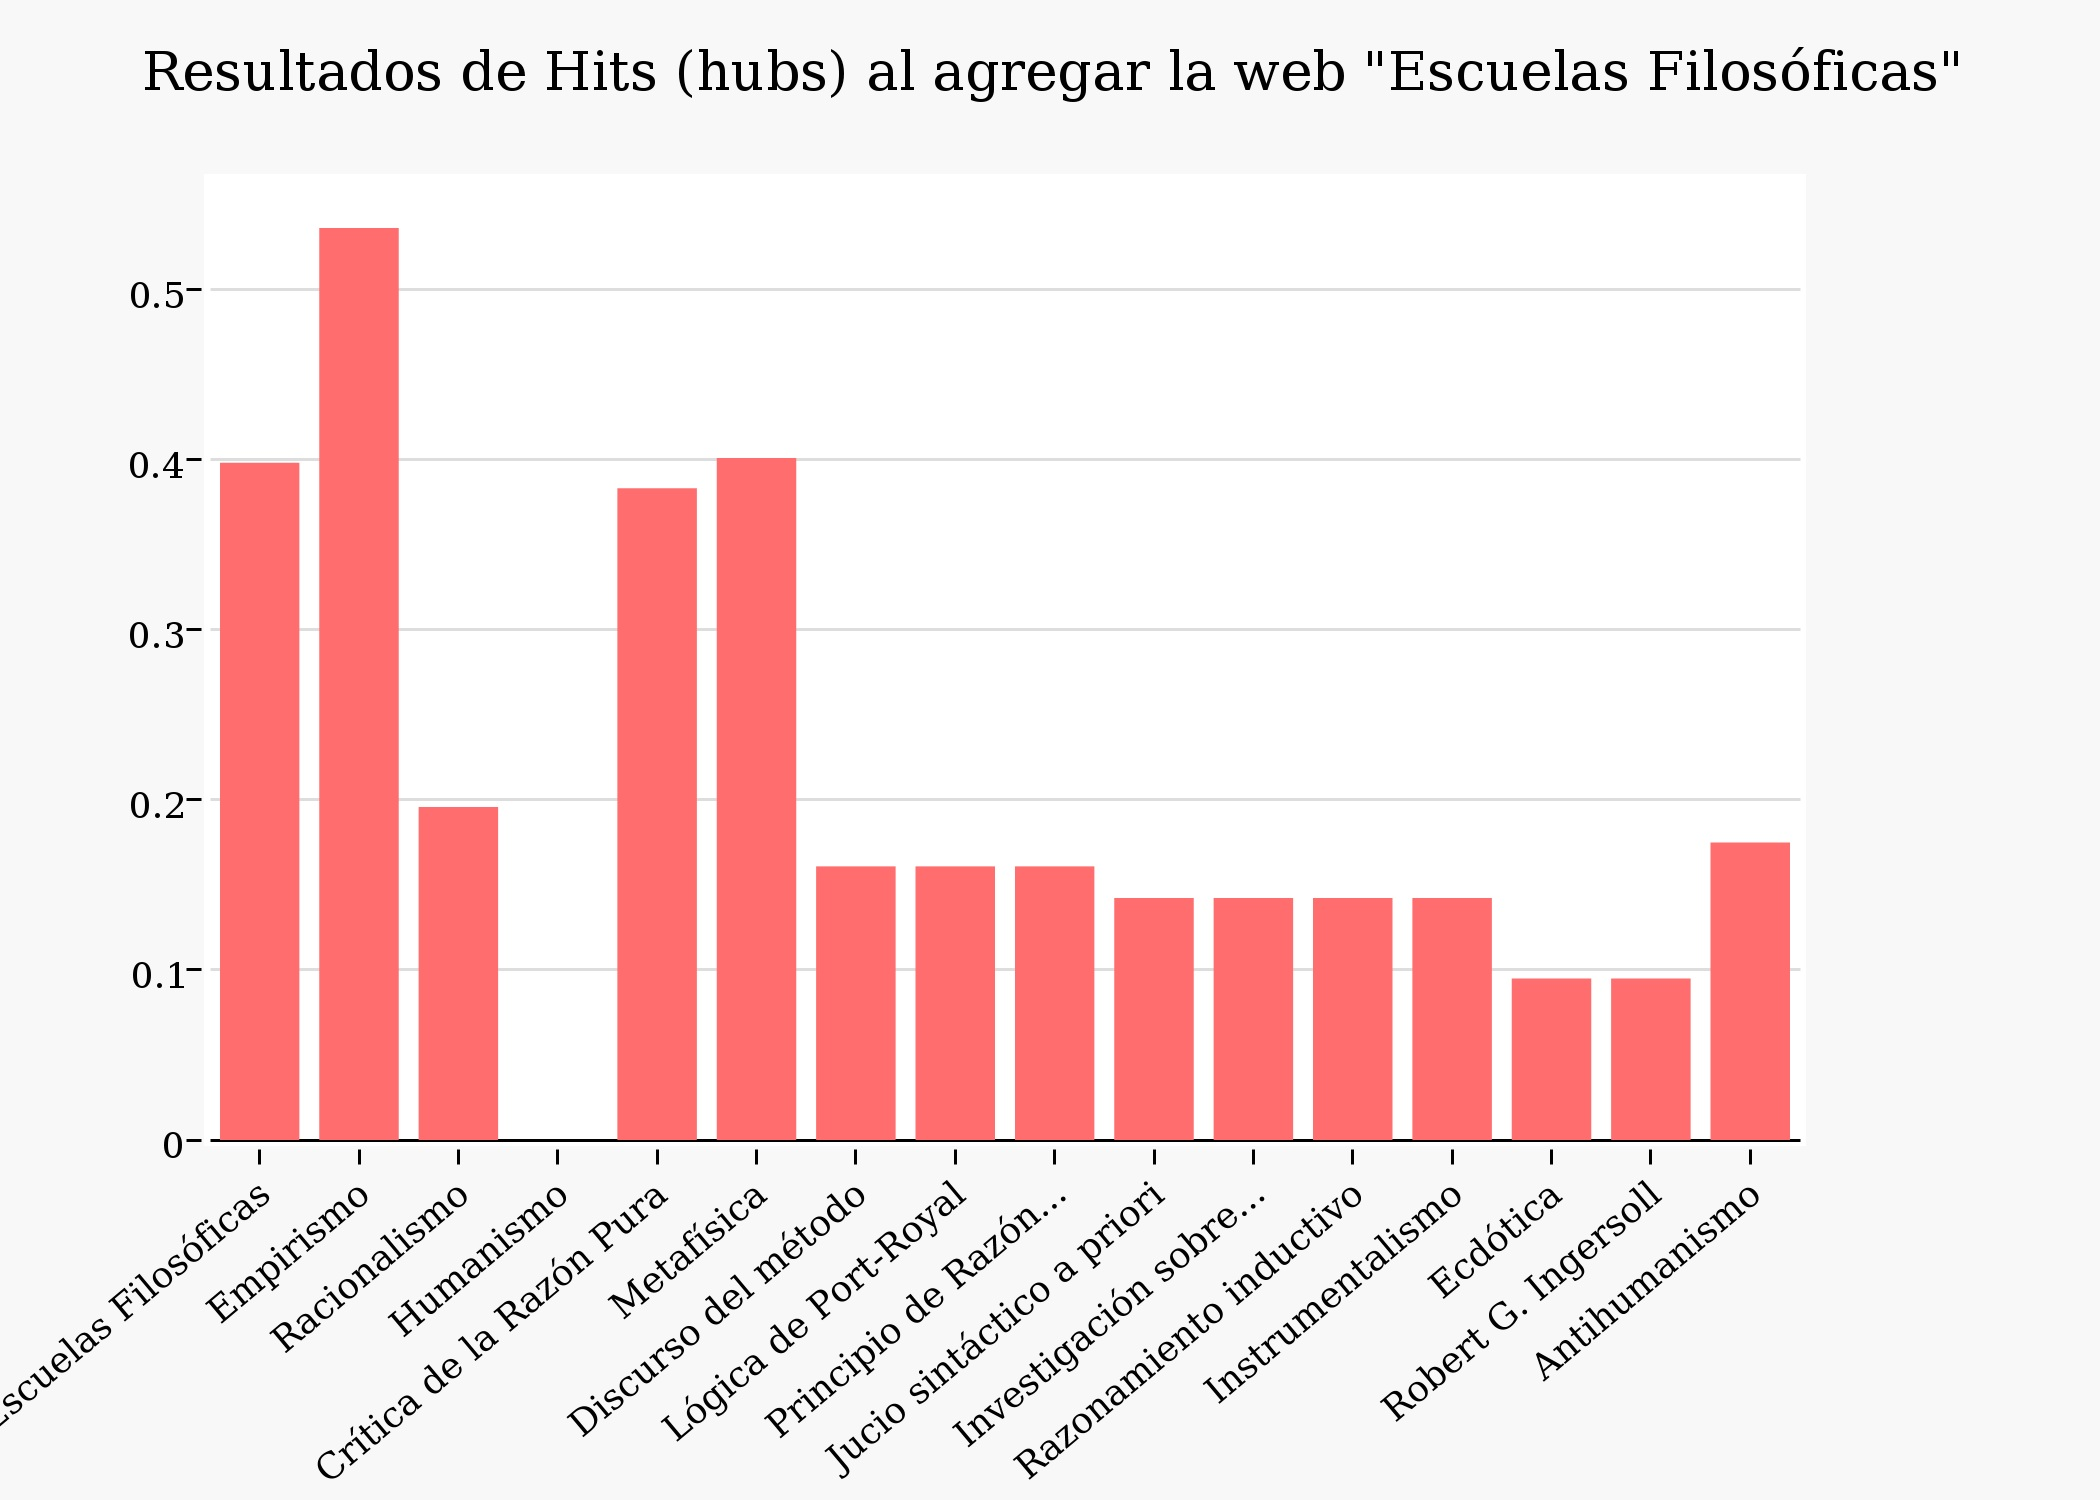
\includegraphics[scale=0.3]{imagenes/Exp2/hitsH2}
	\caption{}
	\label{hitsh2}
  \end{center}
\end{figure}


Si se contrasta la figura \ref{hitsh1} con la figura \ref{hitsh2} (propia de este experimento) se puede ver que el máximo valor de hub  no se realiza en el peso del sitio agregado, sino en los que eran hubs destacados en la red original. \\
Si bien no obtuvimos los resultados esperados (la web agregada no resultó ser el hub más importante), esto pudo deberse a que el peso de hubs preexistentes era de gran magnitud. Al subestimar la dificultad de reemplazar un hub por otro y considerar que bastaría con que la nueva página apuntase a unas pocas pero fuertes autoridades, no tuvimos presente el hecho de que cada link saliente de una página incrementa o mantiene en la misma su valor de hub, sea cual fuere el peso de la página apuntada. Sin tener en cuenta esto, desestimamos la posibilidad de que se constituyera como hub prioritario una web que apuntara a muchas otras de pesos - en principio - poco relevantes, siendo que existía otra que aglutinaba en sus links a varias de las mejores autoridades de la red.

Nos parece importante destacar que a pesar de no haber obtenido estrictamente los resultados esperados, notamos que la nueva red preservó el orden relativo de los hubs de la red inicial a excepción de la nueva página agregada que, a pesar de no haber obtenido el mejor de los valores, fue posicionada entre los hubs de mayor relevancia.\\


\newpage

\textbf{Hipótesis 3: \itshape{Sea A una página de la red apuntada por otra página B perteneciente a la misma. En caso de que se agreguen a la red nuevos nodos a los que B apunte, entonces el nivel de importancia de la web A se verá dismunído en la segunda red de acuerdo al método de PageRank.}}\\

Con el fin de contrastar la presente hipótesis, agregamos a la $Red$ $2$ un conjunto de links salientes de "$Antihumanismo$" (página que apuntaba a "humanismo"), resultando la siguiente red:

\textbf{Red 3:}\\

\begin{tabular}{l l}
1 & Escuela Filosófica \\
2 & Empirismo \\
3 & Racionalismo \\
4 & Humanismo \\
5 & Crítica de la razón pura \\
6 & Metafísica \\
7 & Discurso del método \\
8 & Lógica de Port-Royal \\
9 & Principio de razon suficiente \\
10 & Juicio sintáctico a priori \\
11 & Investigación sobre el entendimiento humano \\
12 & Razonamiento inductivo \\
13 & Instrumentalismo \\
14 & Ecdótica \\
15 & Robert G. Ingersoll \\
16 & Antihumanismo \\
17 & Razón \\
18 & Muerte de Dios \\
19 & Claude Levì-Strauss \\
20 & Michel Foucault \\
\end{tabular}\\

Los resultados obtenidos son los presentados en las figuras \ref{before3}, ~\ref{after3}, mientras que en la figuras ~\ref{gbefore3} se puede observar el grafo de la web inicial.

\begin{figure}[h!]
  \begin{center}
	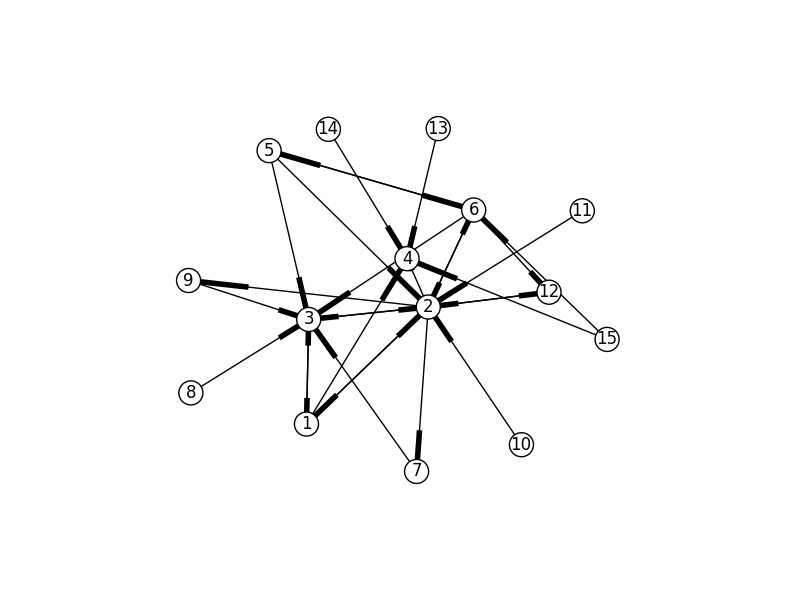
\includegraphics[scale=0.60]{imagenes/Exp3/grafobefore}
	\caption{}
	\label{gbefore3}
  \end{center}
\end{figure}
\newpage
\begin{figure}[h!]
  \begin{center}
	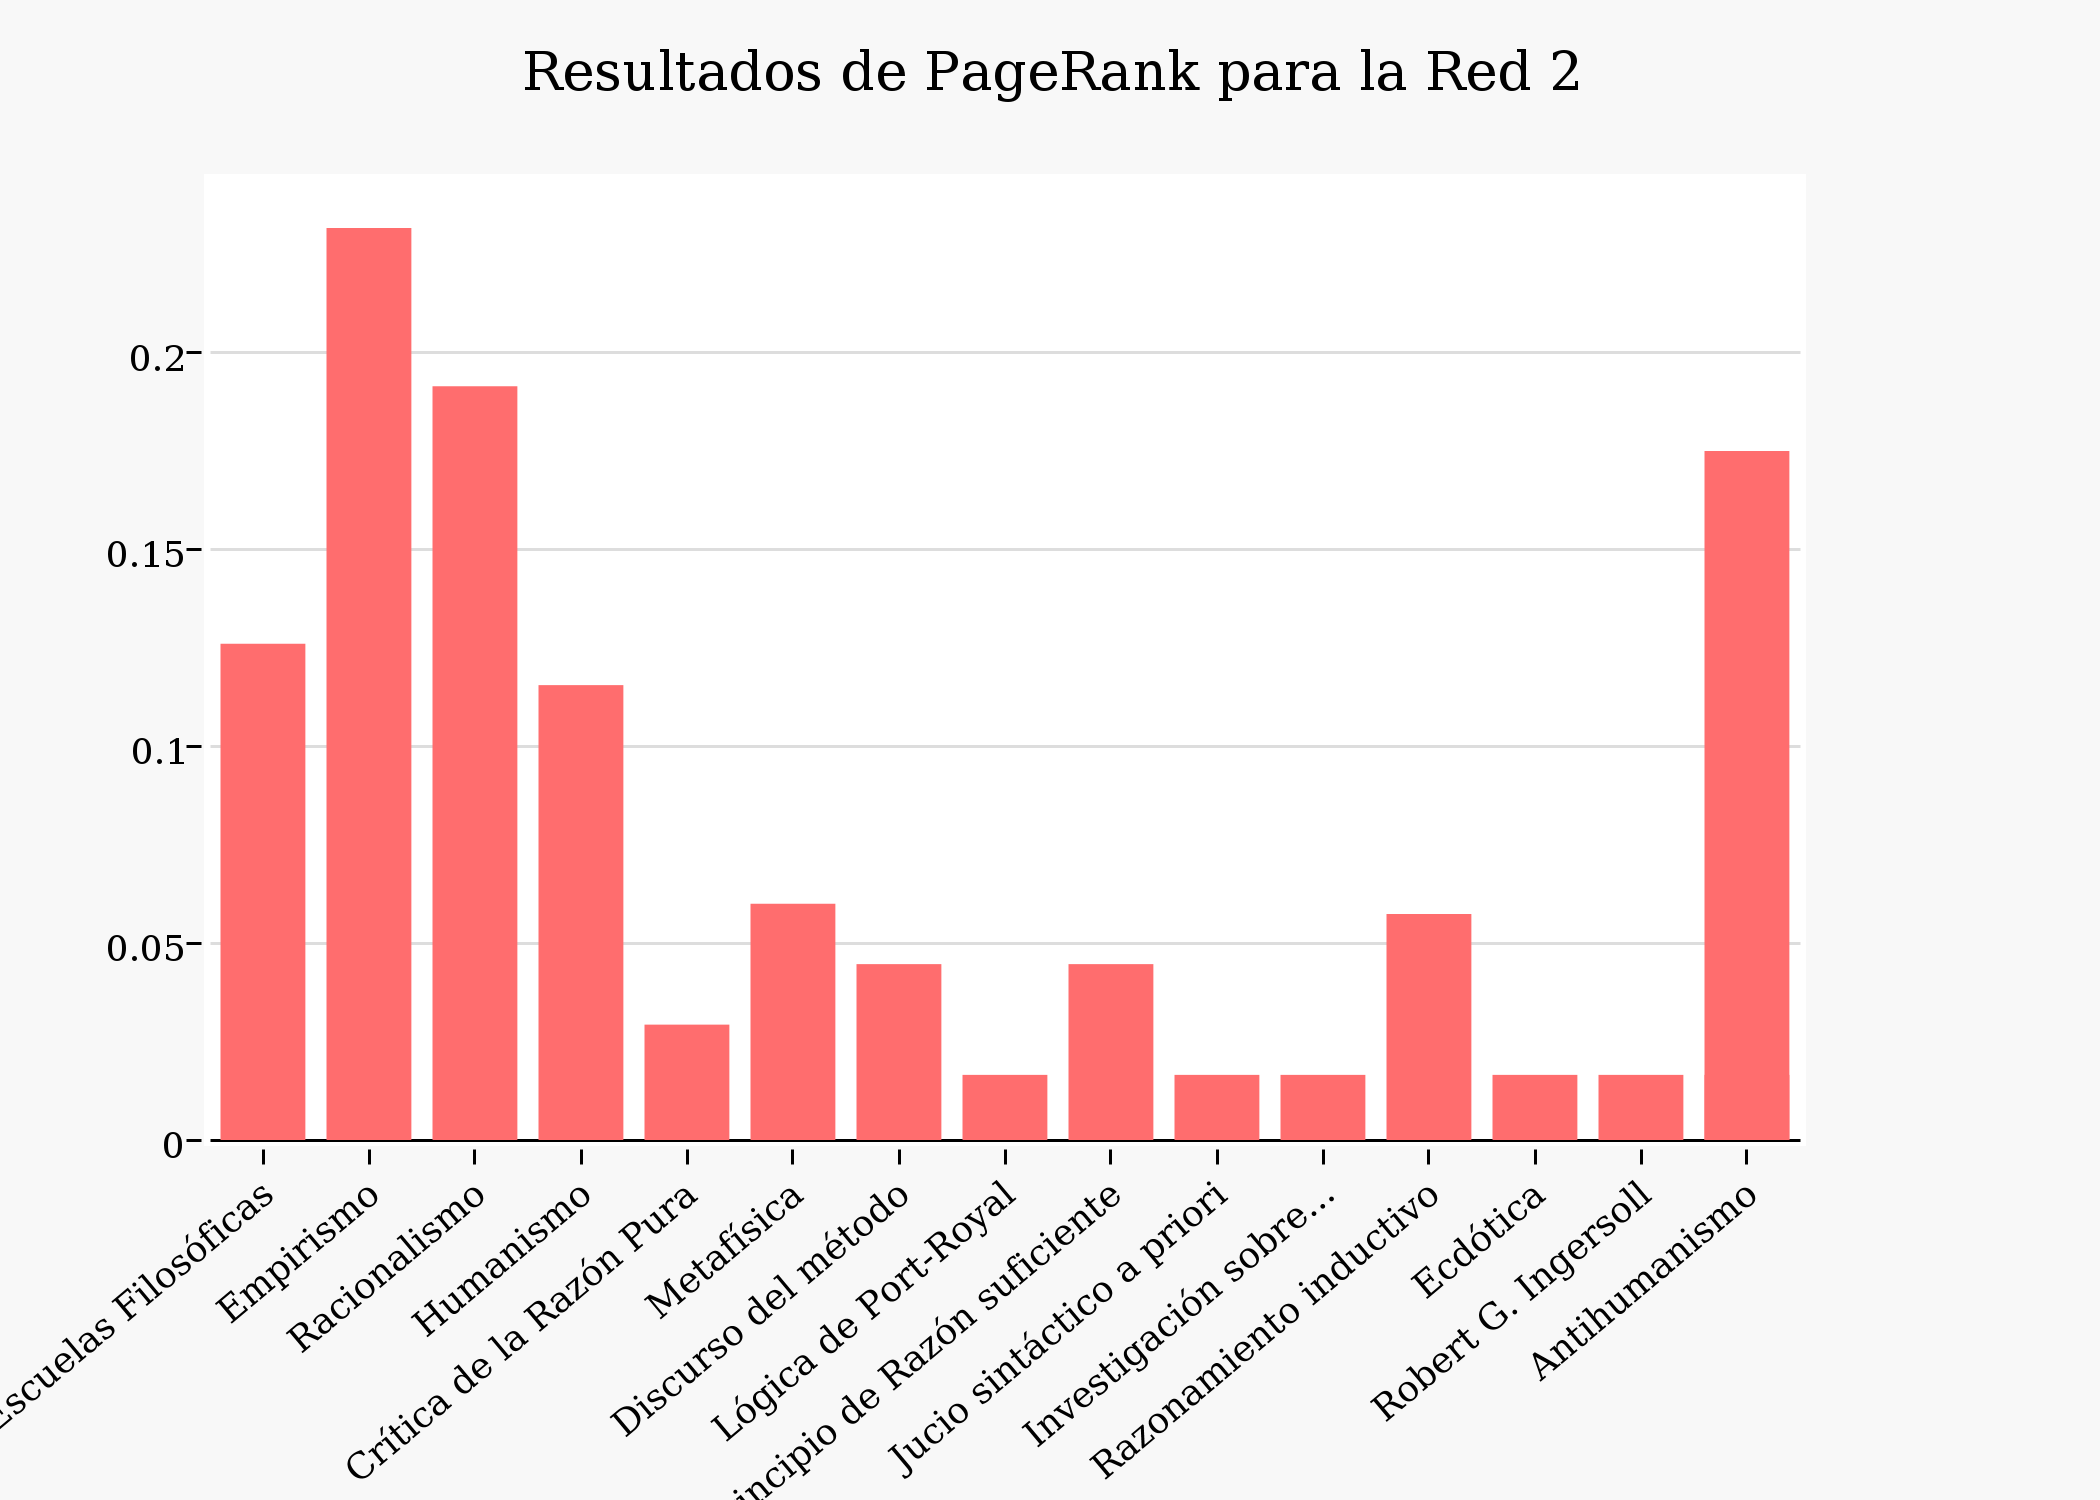
\includegraphics[scale=0.80]{imagenes/Exp3/before}
	\label{before3}
	\caption{Descripcion de la figura}
  \end{center}
\end{figure}

\begin{figure}[h!]
  \begin{center}
	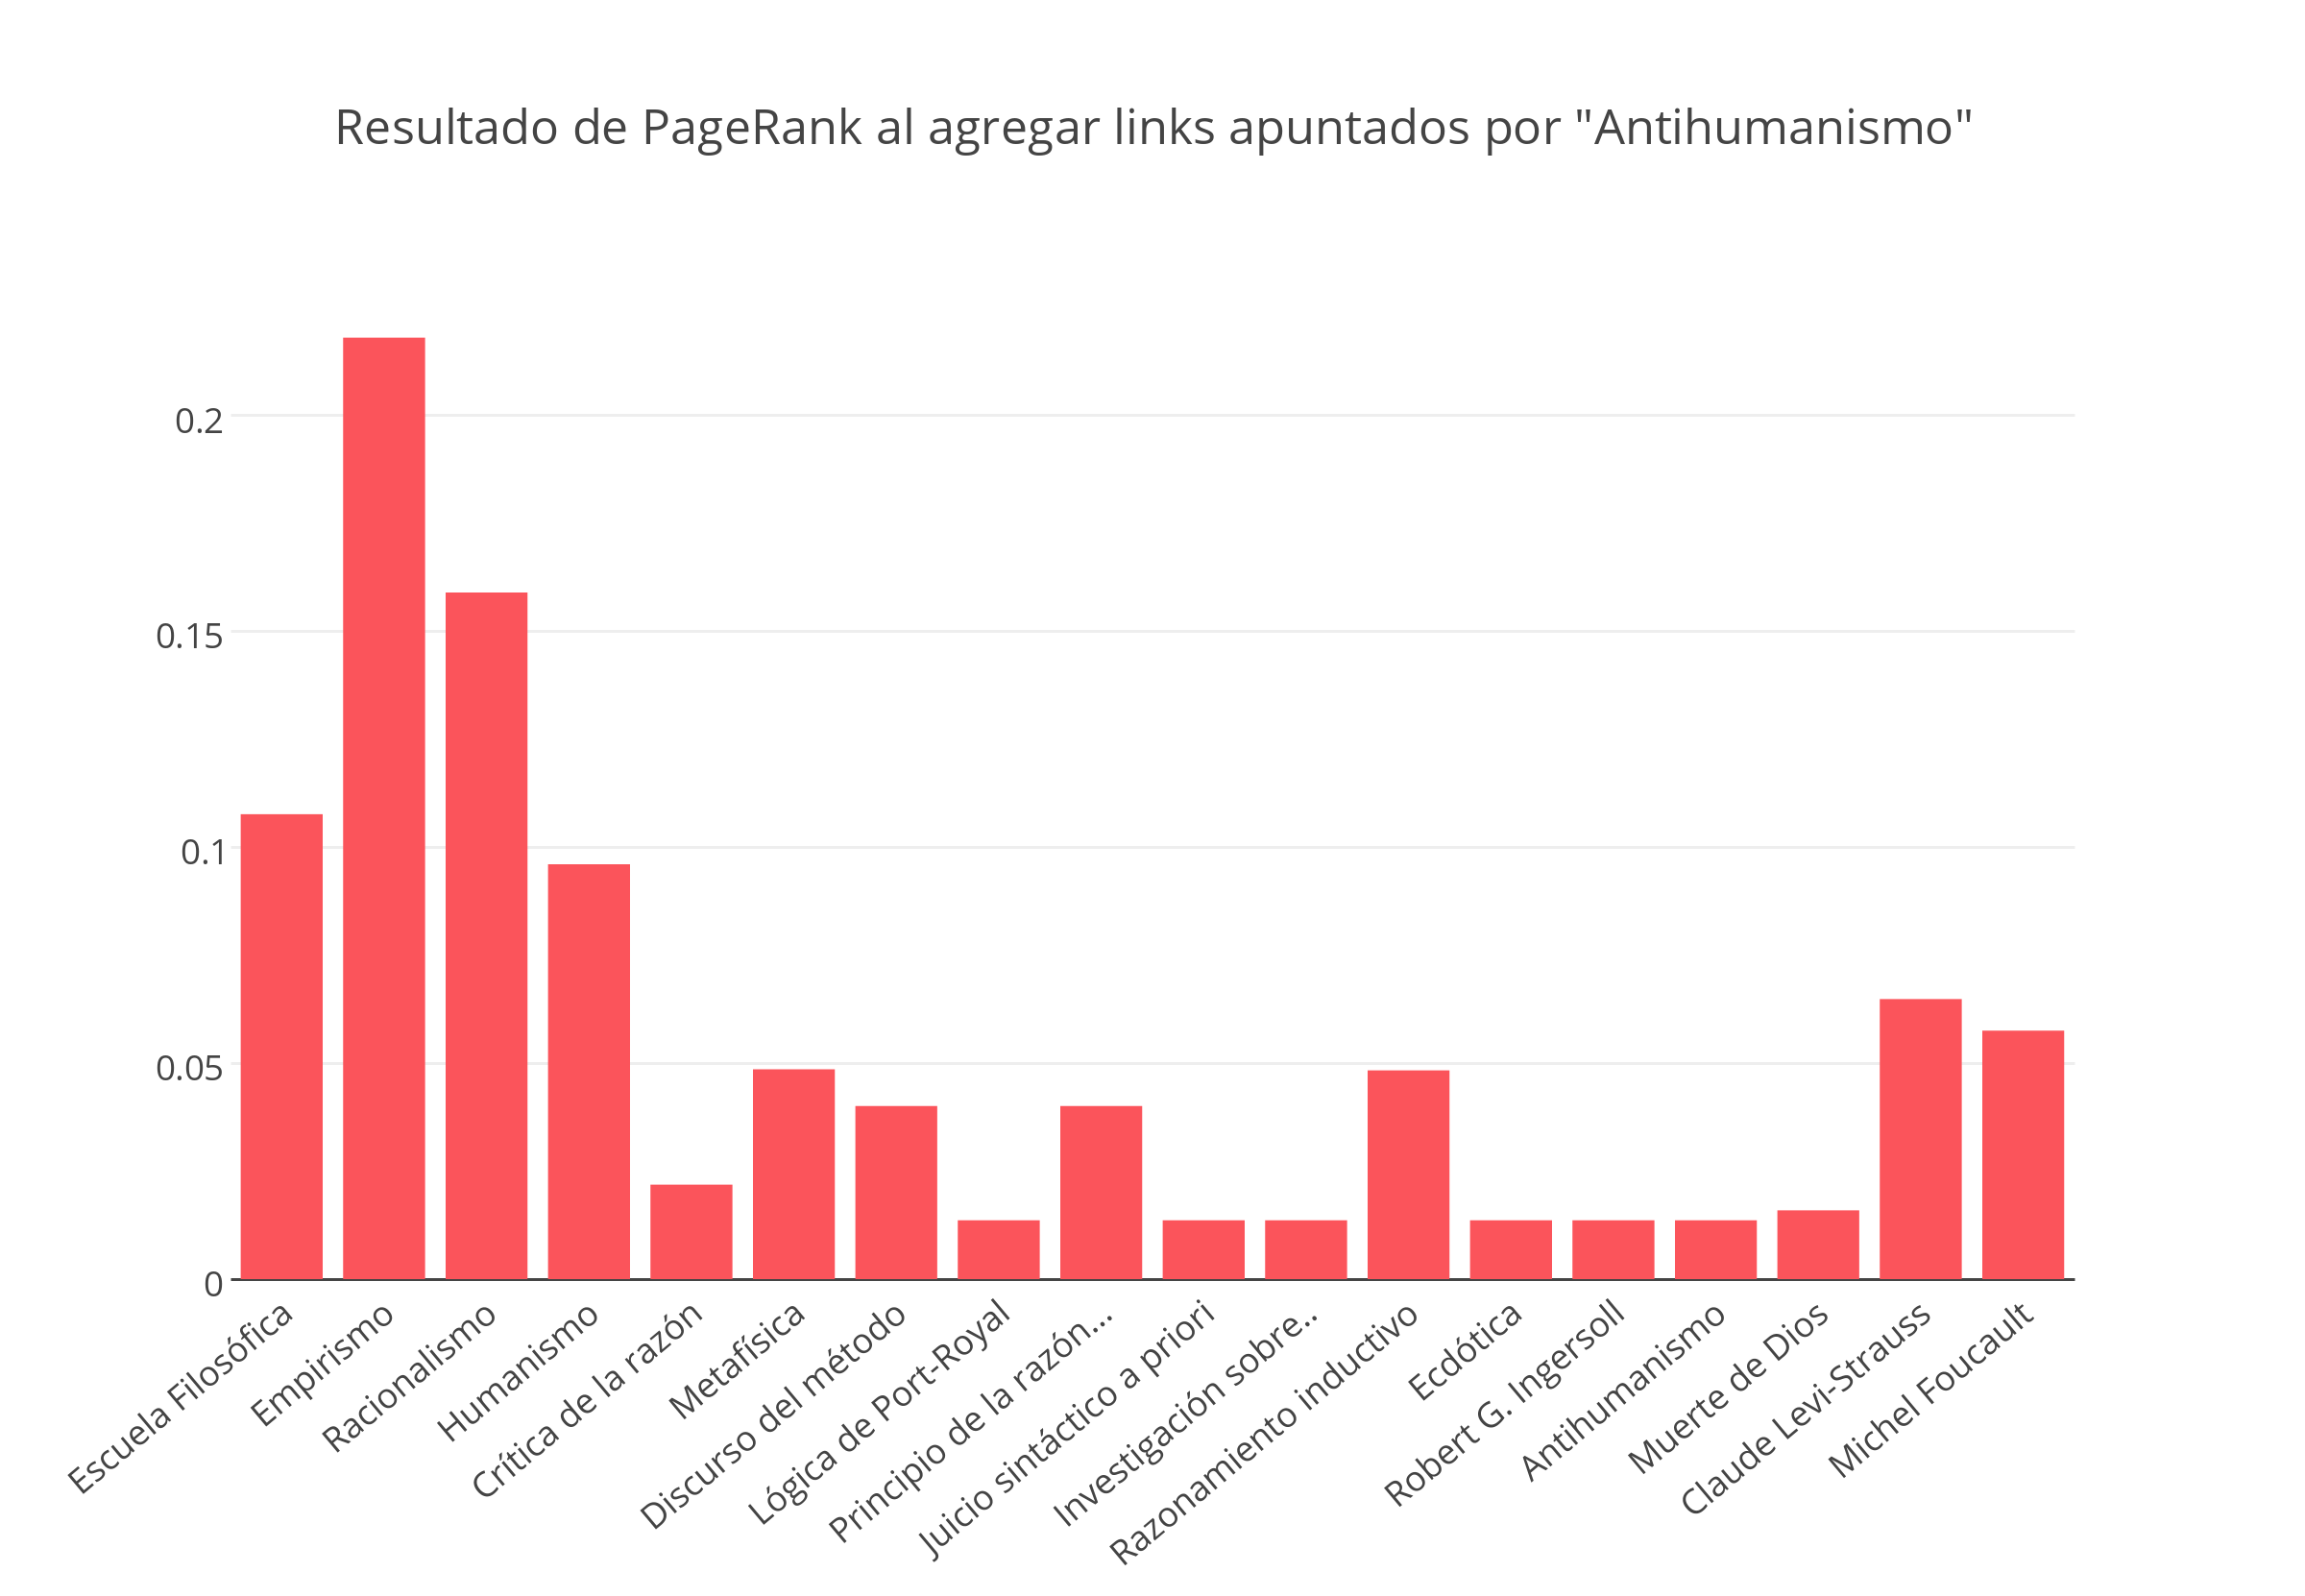
\includegraphics[scale=0.80]{imagenes/Exp3/after}
	\caption{}
	\label{after3}
  \end{center}
\end{figure}
\newpage


\indent Al realizar este experimento, nuestro principal objetivo consistía en averiguar si el incremento de los links salientes de un nodo que apuntara a pocas páginas afectaría a las mismas, decrementando su importancia. Sin embargo, la fluctuación de dichos valores no fue lo más llamativo de la compraración entre el orden dado por PageRank en la red inicial y el dado por el mismo método para la red modificada. \\
\indent Si bien se puede apreciar una diferencia negativa entre el valor de la página de ``humanismo'' entre la primera instancia y la segunda, también es cierto que la mayor parte de los nodos manifiestan este cambio. Esto puede deberse a la imposibilidad de garantizar que todos las modificaciones realizadas sean locales, puesto se cuenta con una red entramada en la cual cada cambio es potencialmente transitivo. \\
\indent Por otro lado, el nodo cuyo valor se disminuyó notablemente fue aquel que incorporó nuevos links salientes. Esto cobra sentido cuando se piensa en la interpretación que se les da a los valores obtenidos en el método analizado: cada uno representa la proporción de tiempo que, en el largo plazo, el navegante aleatorio pasa en dicha página. De esta forma, si se incrementa la cantidad de links salientes de un nodo, se amplía la cantidad de sitios que el navegante aleatorio visitará sin teletransportarse, disminuyendo así el tiempo que el mismo pasará en el nodo en cuestión.


\newpage


\textbf{Hipótesis 4: \itshape{Al aumentar la probilidad de que el navegante aleatorio se transporte, crece también la proporcion de tiempo que se espera que permanezca en paginas que inicialmente no se consideran de gran relevancia.
 }}\\
\textcolor{red}{COMPLETAR TODO}\\

\newpage

\textbf{Hipótesis 5: \itshape{BLA }}\\
\textcolor{red}{LA HIP 5 LA PENSAMOS INICIALMENTE PARA PROBAR MAS O MENOS COMO IBA TODO, SIN HIPOTESIS. QUE PONGO? (ES LA Q SE AGREGA "MATRIZ" A LO ULTIMO)}\\

\newpage
\subsection{Comparaci\'on de la calidad de los Resultados para distintos m\'etodos}
A continuaci\'on se presentan los primeros 6 y 3 resultados de cada ranking.
\subsection*{Abortion}
\indent Al momento de correr los tres algoritmos sobre la red \emph{Abortion} (con 2.293 nodos), los primeros elementos en figurar dentro de los ranking fueron los siguientes: \\
\\
\underline{Pagerank} (bajo un C=0.85): \\
\\
(0.012534) \textbf{The John Birch Society} \\
\textit{http://www.jbs.org} \\
Links entrantes:32 \indent Links salientes: 5\\
\\
(0.009202) \textbf{About - The Human Internet} \\
\textit{http://home.about.com} \\
Links entrantes:30 \indent Links salientes: 0\\
\\
(0.008679)\textbf{ AllExperts.com }\\
\textit{http://www.allexperts.com/about.asp} \\
Links entrantes:55 \indent Links salientes: 1\\
\\
(0.007845) \textbf{American Opinion Book Services Online Store }\\
\textit{http://www.aobs-store.com} \\
Links entrantes:25 \indent Links salientes: 1\\
\\
(0.006514) \textbf{National Right to Life Organization} \\
\textit{http://www.nrlc.org} \\
Links entrantes:184 \indent Links salientes: 1\\
\\
(0.00647) \textbf{TRIMonline - Lower Taxes Through Less Government} \\
\textit{http://www.trimonline.org} \\
Links entrantes:24 \indent Links salientes: 4\\
\\
\\
\underline{In-deg}:\\
\\
(184) \textbf{National Right to Life Organization} \\
\textit{http://www.nrlc.org} \\
Links entrantes:184 \indent Links salientes: 1\\
\\
(126) \textbf{Planned Parenthood Federation of America} \\
\textit{http://www.plannedparenthood.org} \\
Links entrantes:126 \indent Links salientes: 0\\
\\
(115) \textbf{NARAL: Abortion and Reproductive Rights: Choice For Women} \\
\textit{http://www.naral.org }\\
Links entrantes:115 \indent Links salientes: 0\\
\\
(114) \textbf{DimeClicks.com - Complete Web and Marketing Solutions} \\
\textit{http://www5.dimeclicks.com }\\
Links entrantes:114 \indent Links salientes: 0\\
\\
(114)\textbf{ Amazon.com--Earth's Biggest Selection }\\
\textit{http://www.amazon.com/exec/obidos/redirect-home/youdebatecom} \\
Links entrantes:114 \indent Links salientes: 0\\
\\
(114) \textbf{HitBox.com - hitbox web site traffic counter - internet statistics and site promotion tools - WebSideStory} \\
\textit{http://rd1.hitbox.com/rd?acct=WQ590703J6FB45EN5} \\
Links entrantes:114 \indent Links salientes: 0\\
\\
\underline{Hits}: \\
\\
\emph{Mayores Autoridades}: \\
\\
(0.333946) \textbf{DimeClicks.com - Complete Web and Marketing Solutions} \\
\textit{http://www5.dimeclicks.com }\\
Links entrantes:114 \indent Links salientes: 0\\
\\
(0.333946) \textbf{Amazon.com--Earth's Biggest Selection} \\
\textit{http://www.amazon.com/exec/obidos/redirect-home/youdebatecom} \\
Links entrantes:114 \indent Links salientes: 0\\
\\
(0.333946) \textbf{HitBox.com - hitbox web site traffic counter - internet statistics and site promotion tools - WebSideStory} \\
\textit{http://rd1.hitbox.com/rd?acct=WQ590703J6FB45EN5} \\
Links entrantes:114 \indent Links salientes: 0\\
\\
\\
\emph{Mayores Hubs}: \\
\\
(0.095693)\textbf{ Abortion Books Pro and Con} \\
\textit{http://www.4greatbooks.com/abortion-books.htm} \\
Links entrantes:0 \indent Links salientes: 27\\
\\
(0.09428) \textbf{Government Debates and Polls} \\
\textit{http://www.youdebate.com/government.htm }\\
Links entrantes:0 \indent Links salientes: 10\\
\\
(0.09428) \textbf{Political Debates and Polls }\\
\textit{http://www.youdebate.com/POLITICS.htm} \\
Links entrantes:0 \indent Links salientes: 10\\
\\
\\
\indent Es necesario destacar que  la p\'agina \emph{DimeClicks.com} queda en la posici\'on 1 dentro del Ranking de Autoridades de HITS y en la posici\'on 4 en el de In-Deg, cuando esta p\'agina no nos es de inter\'es al momento de hacer una b\'usqueda con el string \textit{``Abortion''} ya que consiste en una p\'agina de Marketing y soluciones Web. En cambio, para PageRank esta p\'agina se sit\'ua en la posici\'on 27 con un puntaje de 0,00318. Adem\'as, la p\'agina que ocupa la tercera posici\'on del Ranking de pesos de autoridad -\emph{HitBox.com}- tampoco est\'a relacionada con el contexto de \emph{Aborto}, ya que habla de promociones y estad\'isticas en Internet. Mientras que HitBox se sit\'ua en la posici\'on 6 para In-Deg y en la posici\'on 27 para PageRank con un puntaje de 0,00318. \\
\indent Por lo tanto, se puede concluir que para estar Red, PageRank sabe filtrar \textit{``mejor''} las p\'aginas que no nos son de ning\'un inter\'es bajo el contexto de b\'usqueda.\\

\subsection*{Movies}
\indent A continuaci\'on se muestran los rankings obtenidos tras correr los tres algoritmos sobre la red \emph{Movies} (con 5.757 nodos), los primeros elementos en figurar dentro de los ranking fueron los siguientes: \\
\\
\\
\underline{PageRank} (bajo un C=0.85): \\
\\
(0.007915)\textbf{ On Wisconsin }\\
\textit{http://www.onwisconsin.com} \\
Links entrantes:127 \indent Links salientes: 8\\
\\
(0.007829) \textbf{GuideLive: Movies in Dallas and Fort Worth }\\
\textit{http://www.guidelive.com/topic/movies.htm} \\
Links entrantes:62 \indent Links salientes: 51\\
\\
(0.007015)\textbf{ citysearch.com} \\
\textit{http://www.citysearch.com }\\
Links entrantes:27 \indent Links salientes: 9\\
\\
\\
\underline{In-Deg}: \\
\\
(393)\textbf{ The Internet Movie Database (IMDb). }\\
\textit{http://www.moviedatabase.com }\\
Links entrantes:393 \indent Links salientes: 0\\
\\
(277) \textbf{Hollywood.com - Your entertainment source for movies, movie showtimes, movie reviews, television and celebrity news.!} \\
\textit{http://www.hollywood.com }\\
Links entrantes:277 \indent Links salientes: 0\\
\\
(143)\textbf{ Paramount Pictures - Home Page} \\
\textit{http://www.paramount.com }\\
Links entrantes:143 \indent Links salientes: 0\\
\\
\\
\underline{HITS}: \\
\\
\emph{Mayores Autoridades}: \\
\\
(0.1412) \textbf{Empty title field} \\
\textit{http://chatting.about.com} \\
Links entrantes:70 \indent Links salientes: 0\\
\\
(0.139835)\textbf{ About.com A-Z} \\
\textit{http://a-zlist.about.com} \\
Links entrantes:48 \indent Links salientes: 0\\
\\
(0.139793) \textbf{About - Arts/Humanities} \\
\textit{http://home.about.com/arts} \\
Links entrantes:47 \indent Links salientes: 0\\
\\
\\
\emph{Mayores Hubs}: \\
\\
(0.159812) \textbf{History of Classic Movies} \\
\textit{http://classicfilm.miningco.com/entertainment/classicfilm/msub19.htm} \\
Links entrantes:0 \indent Links salientes: 73\\
\\
(0.159471)\textbf{ Movie Reviews} \\
\textit{http://movieboxoffice.miningco.com/entertainment/movieboxoffice/msub7.htm} \\
Links entrantes:0 \indent Links salientes: 68\\
\\
(0.159471) \textbf{Characters: Creatures} \\
\textit{http://starwars.miningco.com/entertainment/starwars/msubchar-crea.htm }\\
Links entrantes:0 \indent Links salientes: 68\\
\\
\\
\indent En esta ocasi\'on, tambi\'en se puede apreciar que las p\'aginas con mayor puntaje de autoridad no son las m\'as acertadas para nuestro contexto. Sin embargo, lo m\'as llamativo de este caso es que las p\'aginas con mejor puntaje de Hub resultan ser p\'aginas acertadas para la b\'usqueda, p\'aginas que un usuario podr\'ia estar interesado en encontrarse al momento de buscar el string ``movie''. La p\'agina \emph{History of Classic Movies} queda en la posici\'on 3783 para PageRank y para In-Deg, con un puntaje de Autoridad que lo ubica en la posici\'on 2888. Por otro lado, la p\'agina \emph{Movie Reviews} se ubica en la posici\'on 3771 del ranking de PageRank, tambi\'en en la 3771 de In-Deg y ocupa la posici\'on 2876 con su puntaje de Autoridad.\\
\indent De este modo, se puede concluir que -para la Web Movies- priorizar las p\'aginas con mayor puntaje de Hub por sobre las que tengan mejor puntaje de Autoridad es una buena idea, ya que los resultados obtenidos fueron m\'as cercanos a lo esperado de este modo.\\
\\
\newpage
\section{Conclusiones}
A lo largo del presente trabajo hemos analizado distintos métodos cuyos propósitos consisten en jerarquizar un grupo de páginas interrelacionadas a partir de ciertos criterios y modelos de la realidad. \\
\indent Habiendo formulado nuestras propias hipótesis acerca del comportamiento de dichos métodos y sus puntos fuertes y endebles y habiendo podido experimentar con ellos, nos proponemos en este momento aunar las interpretaciones de cada uno de los resultados obtenidos para elaborar una conclusión que sirva a la resolución del problema planteado.\\
\indent Ante todo es importante destacar que la indicación sugerida por nosotros dependerá del método con el cual se ordenen las páginas web. Es por ello que se enumeran a continuación las estrategias sugeridas para cada uno de los métodos posibles:\\
\\
\indent \textbf{In-deg:} Como ya se vio, para puntuar alto en este modelo basta con conseguir que una gran cantidad de páginas apunten a la propia. Es por ello que en este caso nos remitimos a sugerir que se compren tantos links como sea posible, sin ahondar en profundidad en la importancia relativa de cada página dentro de la red.\\
\\
\indent \textbf{HITS:} En este caso, como la forma de presentar los resultados es devolviendo primero las p\'aginas con mayor puntaje de Autoridad y luego las que tengan mayor puntaje de Hub, nos situamos en aumentar su puntaje de Autoridad. A través de una serie de experimentaciones y análisis notamos que un factor de gran influencia a la hora de aumentar el valor de un nodo como autoridad está dado por la cantidad y calidad de los hubs que lo apuntan. Por este motivo, nuestra recomendación es que el cliente consiga que su página sea apuntada por la mayor cantidad de webs de este tipo, cuyo orden se encuentre entre los principales.\\
\\
\indent  \textbf{PageRank:} Considerando los distintos resultados obtenidos a partir de las pruebas y ensayos constituídos en torno a este método, concluímos que la forma más efectiva de garantizar que mejore la posición de la web del cliente en una red es realizando un análisis de la misma y consiguiendo que la apunten la mayor cantidad posible de sitios que poseen una posición destacada dentro de la misma y que a su vez no apuntan a demasiadas páginas. \\
\indent Este criterio no es arbitrario, dado que el valor que una página transmite a otra depende no sólo de su propio valor sino también de la cantidad de sitios que también se están beneficiando de él. \\
\indent Si esto no fuese posible (por ejemplo porque no existiera en la red una cantidad suficiente de páginas con las características mencionadas), entonces el criterio para discernir de qué manera proseguir debería ser lo suficientemente sutil y detallista como para escoger entre una serie de páginas cuyo peso no sea de una magnitud considerable pero satisfagan tener pocos links salientes, y otro grupo de mayor importancia pero con mayor cantidad de links salientes.\\

\newpage
\section{Ap\'endices}
	\subsection{Ap\'endice A}

		%\documentclass[11pt, a4paper]{article}
	%\usepackage[spanish]{babel}
%\usepackage{a4wide}
%\usepackage{amsfonts}
%\usepackage{graphicx}
%\usepackage{verbatim}
%\usepackage{todonotes}
%\usepackage{amsmath}
%\usepackage{url}

%\usepackage{tikz}
%\usetikzlibrary{decorations.markings,arrows}

\parindent = 0 pt
\parskip = 5 pt

\newcommand{\real}{\hbox{\bf R}}

%\begin{document}
\begin{center}
\begin{tabular}{r|cr}
 \begin{tabular}{c}
{\large\bf\textsf{\ M\'etodos Num\'ericos\ }}\\ 
Segundo Cuatrimestre 2014\\
{\bf Trabajo Pr\'actico 2}\\
\end{tabular} &
\begin{tabular}{@{} p{1.6cm} @{}}

\includegraphics[width=1.6cm]{logodpt.jpg}
\end{tabular} &
\begin{tabular}{l @{}}
 \emph{Departamento de Computaci\'on} \\
 \emph{Facultad de Ciencias Exactas y Naturales} \\
 \emph{Universidad de Buenos Aires} \\
\end{tabular} 
\end{tabular}
\vskip 10pt
\textbf{\Large Tirate un qu\'e, tirate un \emph{ranking}...}
\end{center}

\vskip 10pt
\hrule
\vskip 5pt

\noindent\textbf{Motivaci\'on}
\vskip 5pt

Luego de su repentina y ef\'imera irrupci\'on durante el a\~no 2011, un grupo de la movida tropical\footnote{Por
cuestiones de privacidad, no haremos p\'ublico de qu\'e grupo se trata.} est\'a buscando recuperar la notoriedad y los niveles 
de popularidad otrora alcanzados. El retorno incluye, entre otras cosas, un mega recital gratuito, giras por las
principales \emph{bailantas} y por el interior del pa\'is.\footnote{A riesgo de exponer su edad, los miembros de la c\'atedra 
quieren destacar a aquellos pr\'oceres que llevaron a este g\'enero musical a las primeras planas, como Alcides, Sebasti\'an, 
Miguel \emph{Conejito} Alejandro, R\'afaga, La Nueva Luna, Comanche y, como dejar fuera, al \emph{MAESTRO} Antonio R\'ios.}

Para que toda esta movida sea exitosa, los miembros del grupo han acordado con su \emph{community manager} que, adem\'as de
tener una participaci\'on destacada en Pasi\'on de S\'abado, es necesario que la llegada a trav\'es de los medios electr\'onicos
y las redes sociales sea muy efectiva, al igual que en 2011, alcanzando a la mayor cantidad posible de gente y poder, nuevamente, 
sentarse en el living de \emph{la diva de los tel\'efonos}. La conclusi\'on a la que llegaron es que necesitan que cada vez que 
realiza una b\'usqueda relacionada con la movida tropical, su p\'agina se encuentre entre las primeras que muestran los buscadores.

Con ese motivo, se han contactado con el equipo de R+D de M\'etodos Num\'ericos, donde en la primera reuni\'on el cliente propuso
\emph{comprar clicks en publicidades}. Esta, si bien es una alternativa viable, representa un gasto importante para la escala de
inversi\'on con la que se dispone. Luego de una reuni\'on del equipo t\'ecnico, se les hizo una contrapropuesta:
estudiar el comportamiento de los buscadores y, a cambio de shows libres de costo y presentaciones privadas, buscar en qu\'e
p\'aginas conviene figurar para mejorar el posicionamiento virtual del grupo.
 
\vskip 5pt
\noindent\textbf{Contexto}
\vskip 5pt

A partir de la evoluci\'on de Internet durante la d\'ecada de 1990, el desarrollo de motores de b\'usqueda se ha convertido
en uno de los aspectos centrales para su efectiva utilizaci\'on. Hoy en d\'ia, sitios como Yahoo, Google y Bing ofrecen
distintas alternativas para realizar b\'usquedas complejas dentro de un red que contiene miles de millones de p\'aginas
web. 

En sus comienzos, una de las caracter\'isticas que distngui\'o a Google respecto de los motores de b\'usqueda de la \'epoca
fue la calidad de los resultados obtenidos, mostrando al usuario p\'aginas relevantes a la
b\'usqueda realizada. El esquema general de los or\'igenes de este motor de b\'usqueda es brevemente explicando en 
Brin y Page \cite{Brin1998}, donde se mencionan aspectos t\'ecnicos que van desde la etapa de obtenci\'on de
informaci\'on de las p\'aginas disponibles en la red, su almacenamiento e indexado y su posterior procesamiento,
buscando ordenar cada p\'agina de acuerdo a su importancia relativa dentro de la red. El algoritmo utilizado para esta
\'ultima etapa es denominado PageRank y es uno (no el \'unico) de los criterios utilizados para ponderar la importancia
de los resultados de una b\'usqueda. En este trabajo nos concentraremos en el estudio y desarrollo del algoritmo
PageRank.

\vskip 5pt
\noindent\textbf{Los m\'etodos, Parte I: PageRank}
\vskip 5pt

El algoritmo PageRank se basa en la construcci\'on del siguiente modelo. Supongamos que tenemos una red con $n$ p\'aginas 
web $Web = \{1,\dots,n\}$ donde
el objetivo es asignar a cada una de ellas un puntaje que determine la importancia relativa de la misma respecto de las
dem\'as. Para modelar las relaciones entre ellas, definimos la \emph{matriz de conectividad} $W \in \{0,1\}^{n \times n}$ 
de forma tal que $w_{ij} = 1$ si la p\'agina $j$ tiene un link a la p\'agina $i$, y $w_{ij} = 0$ en caso contrario. 
Adem\'as, ignoramos los \emph{autolinks}, es decir, links de una p\'agina a s\'i misma, definiendo $w_{ii} = 0$. Tomando 
esta matriz, definimos el grado de la p\'agina $j$, $n_j$, como la cantidad de links salientes hacia otras p\'aginas 
de la red, donde $n_j = \sum_{i = 1}^n w_{ij}$. Adem\'as, notamos con $x_j$ al puntaje asignado a la p\'agina $j\in
Web$, que es lo que buscamos calcular.

La importancia de una p\'agina puede ser modelada de diferentes formas. Un link de la p\'agina $u \in
Web$ a la p\'agina $v \in Web$ puede ser visto como que $v$ es una p\'agina importante. Sin embargo, no queremos que una
p\'agina obtenga mayor importancia simplemente porque es apuntada desde muchas p\'aginas. 
Una forma de limitar esto es ponderar los links utilizando la importancia de la p\'agina de origen. En otras palabras,
pocos links de p\'aginas importantes pueden valer m\'as que muchos links de p\'aginas poco importantes. En particular,
consideramos que la importancia de la p\'agina $v$ obtenida mediante el link de la p\'agina $u$ es proporcional a la 
importancia de la p\'agina $u$ e inversamente proporcional al grado de $u$. Si la p\'agina $u$ contiene $n_u$ links,
uno de los cuales apunta a la p\'agina $v$, entonces el aporte de ese link a la p\'agina $v$ ser\'a $x_u/n_u$. Luego,
sea $L_k \subseteq Web$ el conjunto de p\'aginas que tienen un link a la p\'agina $k$. Para cada p\'agina pedimos que
%\begin{eqnarray}
$x_k = \sum_{j \in L_k} \frac{x_j}{n_j},~~~~k = 1,\dots,n.$ %\label{eq:basicmodel}
%\end{eqnarray}
Definimos $P \in$ $\Re$nxn tal que $p_{ij} = 1/n_j$ si $w_{ij} = 1$, y $p_{ij} = 0$ en caso contrario. Luego,
el modelo planteado es equivalente a encontrar un $x\in$ $\Re$n tal que $Px = x$, es
decir, encontrar (suponiendo que existe) un autovector asociado al autovalor 1 de una matriz cuadrada, tal que $x_i \ge
0$ y $\sum_{i = 1}^n x_i = 1$. En
Bryan y Leise \cite{Bryan2006} y Kamvar et al. \cite[Secci\'on 1]{Kamvar2003} se analizan ciertas condiciones que debe
cumplir la red de p\'aginas para garantizar la existencia de este autovector.

Una interpretaci\'on equivalente para el problema es considerar al \emph{navegante aleatorio}. \'Este empieza en una
p\'agina cualquiera del conjunto, y luego en cada p\'agina $j$ que visita sigue navegando a trav\'es de sus links,
eligiendo el mismo con probabilidad $1/n_j$. Una situaci\'on particular se da cuando la p\'agina no tiene links salientes. En
ese caso, consideramos que el navegante aleatorio pasa a cualquiera de las p\'agina de la red con probabilidad $1/n$.
Para representar esta situaci\'on, definimos v $\in$ $\Re$nxn, con $v_i = 1/n$ y $d \in \{0,1\}^{n}$ donde 
$d_i = 1$ si $n_i = 0$, y $d_i = 0$ en caso contrario. La nueva matriz de transici\'on es 
\begin{eqnarray*}
D & = & v d^t \\
P_1 & = & P + D.
\end{eqnarray*}
Adem\'as, consideraremos el caso de que el navegante aleatorio, dado que se encuentra en la p\'agina $j$, decida visitar
una p\'agina cualquiera del conjunto, independientemente de si esta se encuentra o no referenciada por $j$ (fen\'omeno
conocido como \emph{teletransportaci\'on}). Para ello, consideramos que esta decisi\'on se toma con una probabilidad
$c \ge 0$, y podemos incluirlo al modelo de la siguiente forma:
\begin{eqnarray*}
E & = & v \bar{1}^t \\
P_2 & = & cP_1 + (1-c)E,
\end{eqnarray*}
\noindent donde $\bar{1}$ $\in$ $\Re$n es un vector tal que todas sus componenetes valen 1. La matriz resultante
$P_2$ corresponde a un enriquecimiento del modelo formulado en (\ref{eq:basicmodel}). Probabil\'isticamente, la
componente $x_j$ del vector soluci\'on (normalizado) del sistema $P_2 x = x$ representa la proporci\'on del tiempo que,
en el largo plazo, el navegante aleatorio pasa en la p\'agina $j \in Web$.

En particular, $P_2$ corresponde a una
matriz \emph{estoc\'astica por columnas} que cumple las hip\'otesis planteadas en Bryan y Leise \cite{Bryan2006} y
Kamvar et al. \cite{Kamvar2003}, tal que $P_2$ tiene un autovector asociado al autovalor 1, los dem\'as autovalores de
la matriz cumplen $1 = \lambda_1 > |\lambda_2| \ge \dots \ge |\lambda_n|$ y, adem\'as, la dimensi\'on
del autoespacio asociado al autovalor $\lambda_1$ es 1. Luego, la soluci\'on al sistema $P_2 x = x$ puede ser calculada
de forma est\'andar utilizando el m\'etodo de la potencia.

Una vez calculado el ranking, se retorna al usuario las $t$ p\'aginas con mayor ranking.

\vskip 5pt
\noindent\textbf{Los m\'etodos, Parte II: Hyperlink-Induced Topic Search}
\vskip 5pt

Un m\'etodo alternativo es propuesto en Kleinberg \cite{Kleinberg}, denominado \emph{Hyperlink-Induced Topic Search} (HITS). La 
intuici\'on del m\'etodo se basa en el an\'alisis intr\'iniseco de la red, donde una noci\'on de \emph{autoridad} se 
transfiere de una p\'agina a otra mediante los links que las relacionan. El objetivo es, dada una b\'usqueda concreta,
retornar un subconjunto acotado de p\'aginas relevantes. Con este fin, se considera que existen p\'aginas que cumplen un 
rol de \emph{autoridad} sobre un tema espec\'ifico y se busca modelar la relaci\'on entre estas p\'aginas y aquellas que 
apuntan a varias de estas autoridades, denominadas \emph{hubs}. En la pr\'actica, los autores observan que suele existir
una especie de equilibrio en la relaci\'on entre hubs y autoridades, y se busca aprovechar esta relaci\'on para el desarrollo
del algoritmo. Intuitivamente, un buen \emph{hub} es una p\'agina que apunta a muchas autoridades, y una buena \emph{autoridad}
es una p\'agina que es apuntada por muchos \emph{hubs}.

El procedimiento consiste en los siguientes pasos. Dada una b\'usqueda concreta, se utiliza en primer lugar un \emph{buscador}
simple (por ejemplo, basado en texto) para obtener un conjunto acotado de paginas (digamos, 200), llamado \emph{root set}. 
Luego, asumiendo que la estructura de la red es conocida, es busca extender este conjunto agregando p\'aginas que son apuntadas
y que apuntan a las p\'aginas de \emph{root set}, hasta llegar a una sub-red de un tama\~no determinado. En el contexto del
trabajo pr\'actico, asumiremos que este paso ha sido realizado y que contamos con el grafo que considera la sub-red.

Formalmente, y retomando la notaci\'on introducida en la secci\'on anterior, consideramos que las p\'aginas de nuestra sub-red
se encuentran en el conjunto $Web = \{1,\dots,n\}$. Para modelar las relaciones entre las p\'aginas, adoptamos una definici\'on 
similar: consideramos la matriz de adyacencia $A \in \{0,1\}^{n \times n}$ donde $a_{ij} = 1$ si existe un link de la p\'agina
$i$ a la p\'agina $j$.\footnote{Notar que $A = W^t$.} Para cada p\'agina $i \in Web$ se considera el \emph{peso de autoridad} $x_i$ 
y el \emph{peso de hub} $y_i$. Consecuentemente, se definen los vectores x,y $\in$ $\Re$n los vectores de pesos de autoridad
y hubs, respectivamente, y supondremos adem\'as que se encuentran normalizados. Las p\'aginas con mayores valores de $x_i$ e $y_i$
son consideradas mejores \emph{autoridades} y \emph{hubs}, respectivamente.

La relaci\'on mencionada entre los distintos tipos de p\'aginas se expresan num\'ericamente de la siguiente forma. Dados los
vectores $x,y$, la operaci\'on de transferencia de los \emph{hubs} a la autoridad $j \in Web$ puede expresarse de la siguiente forma:
\begin{equation}
x_j = \sum_{i: i \to j} y_i. \label{eq:auth-update}
\end{equation}
An\'alogamente, el peso de un hub est\'a dado por la siguiente ecuaci\'on
\begin{equation}
y_i = \sum_{j: i \to j} x_j. \label{eq:hub-update}
\end{equation}

Las ecuaciones (\ref{eq:auth-update}) y (\ref{eq:hub-update}) podemos expresarlas matricialmente de la siguiente manera:
\begin{eqnarray}
x & = & A^ty \label{eq:auth-update-math} \\
y & = & Ax, \label{eq:hub-update-math} 
\end{eqnarray}
aplicando luego el paso de normalizaci\'on correspondiente. Los autores proponen comenzar con un $y_0$ incial, aplicar estas ecuaciones 
iterativamente y demuestran que, bajo ciertas condiciones, el m\'etodo converge. Finalmente, en base a los rankings obtenimos, se retorna
al usuario las mejores $t$ \emph{autoridades} y los mejores $t$ \emph{hubs}.

\vskip 5pt
\noindent\textbf{Enunciado}
\vskip 5pt

El objetivo del trabajo es experimentar en el contexto planteado utilizando los algoritmos de ranking propuestos. Para ello, se considera
un entorno que, dentro de nuestras posibilidades, simule el contexto real de aplicaci\'on donde se abordan instancias de gran escala (es
decir, $n$, el n\'umero total de p\'aginas, es grande). El archivo tomar\'a como entrada un archivo que especifique el algoritmo, los
par\'ametros del mismo y un puntero al grafo de la red y retorne como resultado el ranking obtenido para cada p\'agina. Los detalles sobre 
el input/output del programa son especificados en la siguiente secci\'on.

El trabajo consistir\'a en estudiar distintos aspectos de los siguientes m\'etodos: PageRank, HITS, e \textsc{In-deg}, \'este \'ultimo consiste
en definir el ranking de las p\'aginas utilizando solamente la cantidad de ejes entrantes a cada una de ellas, orden\'andolos en forma
decreciente. Para tener una descripci\'on m\'as completa de los dos primeros m\'etodos, se propone:
\begin{enumerate}
\item Considerar el trabajo de Kleinberg \cite{Kleinberg} con los detalles sobre HITS, en particular las secciones 1, 2 y 3.
\item Considerar el trabajo de Bryan y Leise \cite{Bryan2006} donde se explica la intuci\'on y algunos detalles t\'ecnicos respecto a PageRank. Adem\'as, 
en Kamvar et al. \cite{Kamvar2003} se propone una mejora del mismo. Si bien esta mejora queda fuera de los alcances del trabajo, en la Secci\'on 1 se
presenta una buena formulaci\'on del algoritmo. En base a su definici\'on, $P_2$ no es una matriz esparsa. Sin embargo, en Kamvar et al. 
\cite[Algoritmo 1]{Kamvar2003} se propone una forma alternativa para computar $x^{(k+1)} = P_2 x^{(k)}$. Este resultado puede ser utilizado
para mejorar el almacenamiento de los datos.
\item (Opcional) Completar la demostraci\'on del Teorema 3.1 de Kleinberg \cite{Kleinberg}, incluyendo el detalle de los puntos que el autor asume como 
triviales.
\end{enumerate}

En la pr\'actica, el grafo que representa la red de p\'aginas suele ser esparso, es decir, una p\'agina posee relativamente pocos links
de salida comparada con el n\'umero total de p\'aginas. A su vez, dado que $n$ tiende a ser un n\'umero muy grande, es importante tener
en cuenta este hecho a la hora de definir las estructuras de datos a utilizar. Luego, desde el punto de vista de implementaci\'on se pide
utilizar alguna de las siguientes estructuras de datos para la representaci\'on de las matrices esparsas: \emph{Dictionary of Keys} (dok), 
\emph{Compressed Sparse Row} (CSR) o \emph{Compressed Sparse Column} (CSC). Se deber\'a incluir una justificaci\'on respecto a la elecci\'on 
que consdiere el contexto de aplicaci\'on. Una vez definida la estructura a utilizar, se deber\'a implementar el algoritmo HITS utilizando
las ecuaciones (\ref{eq:auth-update-math}) y (\ref{eq:hub-update-math}). Para el caso de PageRank, se debe implementar el m\'etodo de la
potencia para calcular el autovector principal.

En funci\'on de la experimentaci\'on, se deber\'a realizar un estudio particular para cada algoritmo (tanto en t\'erminos de comportamiento
del mismo, como una evaluaci\'on de los resultados obtenidos) y luego se proceder\'a a comparar cualitativamente los rankings generados.
La experimentaci\'on deber\'a incluir como m\'inimo los siguientes experimentos:
\begin{enumerate}
\item Estudiar la convergencia de PageRank, analizando la evoluci\'on de la norma Manhattan (norma $L_1$) entre dos iteraciones sucesivas. Comparar
los resultados obtenidos para al menos dos instancias de tama\~no mediano-grande, variando el valor de $c$. Opcional: Establecer una relaci\'on 
con la proporci\'on entre $\lambda_1 = 1$ y $|\lambda_2|$.
\item Estudiar la convergencia de los vectores de peso $x$ e $y$ para HITS de forma similar al punto anterior.
\item Estudiar el tiempo de c\'omputo requerido por PageRank y HITS. Si bien ambos pueden se aplicados sobre una red gen\'erica, cada algoritmo 
tiene un contexto particular de aplicaci\'on. Estudiar como impacta el factor temporal en este sentido.
\item Estudiar cualitativamente los rankings obtenidos por los tres m\'etodos. Para ello, se sugiere considerar distintos ejemplos de b\'uquedas
de p\'aginas web\footnote{La c\'atedra adjunta casos de \emph{benchmark} que representan sub-redes obtenidas en base a b\'usquedas tem\'aticas}.
Analizar los resultados individualmente en una primera etapa, y luego realizar un an\'alisis comparativo entre los tres rankings obtenidos.
\item Para cada algoritmo, proponer ejemplos de tama\~no peque\~no que ilustren el comportamiento esperado (puede ser utilizando las instancias
provistas por la c\'atedra o generadas por el grupo).
\end{enumerate}

Finalmente, y en base a la experimentaci\'on realizada, buscamos resolver el problema planteado originalmente: dada una foto de la red, con sus
interconexiones entre p\'aginas, supongamos que tenemos los pesos (ranking) asignados por uno de los algoritmos estudiados. ?`Cu\'al ser\'ia la
estrategia que le sugiere al cliente para mejorar su correspondiente ranking? Para este \'ultimo punto, suponer que es posible \emph{negociar}
que una p\'agina apunte a nuestro sitio, y que la cantidad de estas negociaciones que podemos tener es acotada.

\vskip 5pt
\noindent\textbf{Par\'ametros y formato de archivos}
\vskip 5pt

El programa deber\'a tomar por l\'inea de comandos dos par\'ametros. El primero de ellos contendr\'a la informaci\'on del experimento, incluyendo
el m\'etodo a ejecutar (\verb+alg+, 0 para PageRank, 1 para HITS, 2 para \textsc{In-deg}), la probabilidad de teletransportaci\'on $c$ en el caso
de PageRank (que valdr\'a -1 si \verb+alg+ no es 0), el tipo de instancia, el \emph{path} al archivo/directorio conteniendo la definici\'on de la red (que debe ser relativa
al ejecutable, o el path absoluto al archivo) y el valor de 
tolerancia utilizado en el criterio de parada impuesto a cada m\'etodo. El siguiente ejemplo muestra un caso donde se pide ejecutar PageRank, con una
probabilidad de teletransportaci\'on de 0.85, sobre la red descripta en \verb+red-1.txt+ (que se encuentra en el directorio \verb+tests/+) y con una 
tolerancia de corte de $0.0001$.
\begin{verbatim}
0 0.85 0 tests/red-1.txt 0.0001
\end{verbatim}

Para la definici\'on del grafo que representa la red, se consideran dos bases de datos de instancias con sus correspondientes formatos. La primera
de ellas es el conjunto provisto en SNAP \cite{SNAP} (el tipo de instancia es 0), con redes de tama\~no grande obtenidos a partir de datos reales. Adem\'as, se consideran las 
instancias propuestas en \cite{dataset}. Estas instancias son de tama\~no mediano, obtenidas tambi\'en en base a datos reales, y corresponden a redes
tem\'aticas obtenidas a partir de una b\'usqueda particular. Para cada nodo de la red se tiene: la direccion URL, una breve descripci\'on, y las 
p\'aginas a las cuales apunta. Si bien algunas de las URL ya no son v\'alidas, la descripci\'on permite tener algo m\'as de informaci\'on para 
realizar un an\'alisis cualitativo.

En el caso de la base de SNAP, los archivos contiene primero cuatro l\'ineas con informaci\'on sobre la instancia (entre ellas, $n$ y la cantidad
total de links, $m$) y luego $m$ l\'ineas con los pares $i$, $j$ indicando que $i$ apunta a $j$. A modo de ejemplo, a continuaci\'on se muestra el 
archivo de entrada correspondiente a la red propuesta en Bryan y Leise \cite[Figura 1]{Bryan2006}: 

\begin{verbatim}
# Directed graph (each unordered pair of nodes is saved once): 
# Example shown in Bryan and Leise.
# Nodes: 4 Edges: 8 
# FromNodeId    ToNodeId
1   2
1   3
1   4
2   3
2   4
3   1
4   1
4   3
\end{verbatim}

Para la otras instancias, en \cite{dataset} puede encontrarse una descripci\'on del formato propuesto (el tipo de instancia ser\'a 1 en este caso).

Una vez ejecutado el algoritmo, el programa deber\'a generar un archivo de salida que contenga una l\'inea por cada
p\'agina ($n$ l\'ineas en total), acompa\~nada del puntaje obtenido por el algoritmo PageRank/\textsc{In-deg}. En el caso de HITS, el archivo 
contendr\'a $2n$ l\'ineas, las primeras $n$ con el \emph{peso de autoridad} y las segundas $n$ con el \emph{peso de hub} para los v\'ertices
$1,\dots.n$.

Para generar instancias, es posible utilizar el c\'odigo Python provisto por la c\'atedra. La utilizaci\'on del mismo se
encuentra descripta en el archivo README. Es importante mencionar que, para que el mismo funcione, es
necesario tener acceso a Internet. En caso de encontrar un bug en el mismo, por favor contactar a los docentes de la
materia a trav\'es de la lista. Desde ya, el c\'odigo puede ser modificado por los respectivos grupos agregando todas
aquellas funcionalidades que consideren necesarias.

\vskip 5pt

\hrule

\vskip 5pt


{\bf \underline{Fechas de entrega}}
\begin{itemize}
 \item \emph{Formato Electr\'onico:} S\'abado 11 de Octubre de 2014, hasta las 23:59 hs, enviando el trabajo (informe +
 c\'odigo) a la direcci\'on \verb+metnum.lab@gmail.com+. El subject del email debe comenzar con el texto \verb+[TP2]+
 seguido de la lista de apellidos  de los integrantes del grupo.
 \item \emph{Formato f\'isico:} Mi\'ercoles 15 de Octubre de 2014, a las 17 hs. en la clase te\'orica.
\end{itemize}

\noindent \textbf{Importante:} El horario es estricto. Los correos recibidos despu\'es de la hora indicada ser\'an considerados re-entrega.  

\bibliographystyle{plain}
\bibliography{tp2}
%\end{document}


\newpage
	\subsection{Ap\'endice B}
Se adjunta aqu\'i el algoritmo realizado para insertar, de a un elemento, los valores distintos de cero de una matriz en nuestra matriz esparsa: \\

\IncMargin{1em}
\begin{algorithm}
\SetKwData{Left}{left}\SetKwData{This}{this}\SetKwData{Up}{up}
\SetKwFunction{Union}{Union}\SetKwFunction{FindCompress}{FindCompress}
\SetKwInOut{Input}{input}\SetKwInOut{Output}{output}

\Input{Int fil, Int col, Double elem}
\Output{Void}
\BlankLine

i $\leftarrow$ \'indice donde comienza la fila fil pasada como par\'ametro \\
fin $\leftarrow$ \'indice donde comienza la fila siguiente a la pasada como par\'ametro \\
Iterador itval $\leftarrow$ crear iterador del vector val \\
Iterador itcol $\leftarrow$ crear iterador del vector ind_col \\
\While{(i$<$fin $\wedge$ col$>$itcol )}{
	Avanzar los dos iteradores \\
	i++
}
\eIf{(i == tama\~no del vector ind_col)}{ 
			insertar al final de ind_col el valor col pasado como par\'ametro \\
			insertar al final de val el valor elem pasado como par\'ametro
		}{
			insertar en la posici\'on correspondiente al iterador el valor col pasado por par\'ametro en el vector ind_col \\
			insertar en la posici\'on correspondiente al iterador el valor elem pasado por par\'ametro en el vector val \\
		}
\For{$i\leftarrow fil+1$ \KwTo $cantidad de filas$}{
	ptr_fil[i] ++ 
}
\end{algorithm}\DecMargin{1em}
	\subsection{Ap\'endice C}
El siguiente es un ejemplo de una matriz $A$ $\in$ $\mathbb{R}^{4x4}$ y su traspuesta con su forma de implementaci\'on.\\
\begin{equation}
A = \left(
\begin{array}{cccc}
1 & 0 & 2 & 0 \\
3 & 4 & 0 & 8 \\
0 & 0 & 9 & 0 \\
10 & 11 & 0 & 0
\end{array}
\right)
\end{equation}
 \underline{CSR}:\\
 \indent \indent val = \indent \indent  [1,2,3,4,8,9,10,11]\\
 \indent \indent ind_col = \indent [0,2,0,1,3,2,0,1]\\
 \indent \indent ptr_fil = \indent [0,2,5,6,8]\\
 \underline{CSC}:\\
 \indent \indent val = \indent \indent [1,3,10,4,11,2,9,8]\\
 \indent \indent ind_fil = \indent [0,1,3,1,3,0,2,1]\\
 \indent \indent ptr_col = \indent [0,3,5,7,8]\\
\begin{equation}
A^t = \left(
\begin{array}{cccc}
1 & 3 & 0 & 10 \\
0 & 4 & 0 & 11 \\
2 & 0 & 9 & 0 \\
0 & 8 & 0 & 0
\end{array}
\right)
\end{equation}
 \underline{CSR}:\\
 \indent \indent val = \indent \indent [1,3,10,4,11,2,9,8]\\
 \indent \indent ind_col = \indent [0,1,3,1,3,0,2,1]\\
 \indent \indent ptr_fil = \indent [0,3,5,7,8]\\
 \underline{CSC}:\\
 \indent \indent val = \indent \indent  [1,2,3,4,8,9,10,11]\\
 \indent \indent ind_fil = \indent [0,2,0,1,3,2,0,1]\\
 \indent \indent ptr_col = \indent [0,2,5,6,8]\\
 \\
 En este ejemplo, se puede apreciar que al trasponer la matriz los arreglos conservan sus mismos valores, s\'olo que cambia la forma de interpretarlos. Es decir: ind_fil pasa a ser ind_col, ptr_col pasa a ser ptr_fil y viceversa.
\newpage
\section{Referencias}
\noindent
$[1]$ \indent http://www.cs.toronto.edu/~tsap/experiments/datasets/. \\
\\
$[2]$ \indent Stanford large network dataset collection. http://snap.stanford.edu/data/\#web. \\
\\
$[3]$ \indent Sergey Brin and Lawrence Page. The anatomy of a large-scale hypertextual Web search
engine. Computer Networks and ISDN Systems, 30(1-7):107{117, April 1998. \\
\\
$[4]$ \indent Kurt Bryan and Tanya Leise. The linear algebra behind google. SIAM Review, 48(3):569{
581, 2006. \\
\\
$[5]$ \indent Sepandar D. Kamvar, Taher H. Haveliwala, Christopher D. Manning, and Gene H. Golub.
Extrapolation methods for accelerating pagerank computations. In Proceedings of the 12th
international conference on World Wide Web, WWW '03, pages 261{270, New York, NY,
USA, 2003. ACM. \\
\\
$[6]$ \indent Jon M. Kleinberg. Authoritative sources in a hyperlinked environment. J. ACM,
46(5):604{632, September 1999.

\end{document}

\begin{figure}
  \begin{center}
	
\includegraphics[scale=0.66]{imagenes/logouba.jpg}
	\caption{Descripcion de la figura}
	\label{nombreparareferenciar}
  \end{center}
\end{figure}


%\paragraph{\textbf{Titulo del parrafo} } Bla bla bla bla.
%Esto se muestra en la figura~\ref{nombreparareferenciar}.



%\begin{codesnippet}
%\begin{verbatim}

%struct Pepe {

%    ...

%};

%\end{verbatim}
%\end{codesnippet}